% $Id$
\documentclass[letterpaper,10pt]{book}

\usepackage[T1]{fontenc}
\usepackage[latin1]{inputenc}
\usepackage{geometry}
\usepackage{graphicx,color}
\geometry{letterpaper}

% Enable indexing
\usepackage{makeidx}
\makeindex

% Allows alignment of multiple columns of text
\usepackage{array}

% Enables text wrapping around small tables and figures
\usepackage{float}

% Enables text wrapping around small tables and figures
\usepackage{floatflt}

% Enables side by side figures
\usepackage[countmax]{subfloat}

% Enables line numbering for verbatim text
\usepackage{lineno}

% Some text listing help for script files
\usepackage{listings}
\lstset{frame=single, captionpos=b, language=Matlab, xleftmargin=36pt, xrightmargin=36pt,
basicstyle=\ttfamily, numberstyle=\tiny, numbers=none}

% Use special characters defined by the ams
\usepackage{amsmath}

% Allow rotating figures
\usepackage{lscape}

% Enable verbatiminput so functional script files can be read in directly
\usepackage{fancyvrb}

% Fixes some font sizing problems
\usepackage{fix-cm}

%  for making index, using landscape mode, for multi page tables, supertabular??
% This package is needed to include the tables in the GMATDocuments/common subfolder
\usepackage{longtable, supertabular, multirow, colortbl, color}
\definecolor{lightgray}{rgb}{0.2,0.2,0.2}

%\usepackage{rotating}  %This breaks the png files in \includegraphics{} calls???

% Used for table organization
\usepackage{tabularx}

%\usepackage[listofnumwidth=5.5em]{subfig}

% Used to customize table and figure list spacings
\usepackage{tocloft}

% Used to customize captions
\usepackage{caption}

% for creating bookmarks in the final pdf file when using dvipdfm
\usepackage[dvipdfm, bookmarks = true, bookmarksopen]{hyperref}

%% Used to build enumerations of the form 1.2.3.4.  etc.
%\usepackage[pointedenum]{paralist}

% If going through postscript to pdf, use the following instead for bookmarks:
%\usepackage[dvips, bookmarks = true, bookmarksopen]{hyperref}

%% Used to build the glossary and acronym definitions
%\usepackage[toc]{glossaries}

% Construct the basic page sizes
\oddsidemargin  0.0in
\evensidemargin 0.0in
\textwidth      6.5in
\headheight     0.25in
\topmargin      0.0in
\textheight=8.5in

% Note that png and jpg extensions are used for graphics
\DeclareGraphicsExtensions{.png,.jpg}

%% The following lines customize spacing on the tables of contents, list of figures, etc.
% More space for figure numbers
\setlength{\cftfignumwidth}{3em}
% Space between elements of the list
%\setlength{\cftbeforefigskip}{0.1cm}
% Space before chapter entries in the TOC
%\setlength{\cftbeforechapskip}{0.2cm}
% Space before parts in the TOC
%\setlength{\cftbeforepartskip}{0.7cm}

%\setlength{\emergencystretch}{6em}
%\pretolerance=10000
%\tolerance=10000

%\define@key{caption}{listofnumwidth}[4em]{\def\sf@numwidth{#1}}


\title{The General Mission Analysis Tool (GMAT)\\Estimation Component Architectural
Specification\\(\textit{Architectural Specification Volume II})}
\author{The GMAT Development Team}
%\includeonly{Solvers}
%-------------------------------------------------------------------------------
%------------------------------------New Commands-------------------------------
%-------------------------------------------------------------------------------
\newcommand{\st}[1]{\begin{ttfamily}#1\end{ttfamily}}
\newcommand{\boldst}[1]{\begin{ttfamily}\textbf{#1} \end{ttfamily}}
\newcommand{\br}[0]{$\mathbf{r} $}
\newcommand{\bv}[0]{$\mathbf{v} $}
\newcommand{\ba}[0]{$\mathbf{a} $}
\newcommand{\mbr}[0]{\mathbf{r} }
\newcommand{\mbv}[0]{\mathbf{v} }
\newcommand{\mba}[0]{\mathbf{a} }
\newcommand{\mc}[3]{\multicolumn{#1}{#2}{#3}}


%-------------------------------------------------------------------------------
%------------------------------------New Environments---------------------------
%-------------------------------------------------------------------------------

\newenvironment{ScriptType}
  {\noindent \begin{ttfamily}}
   { \end{ttfamily} }

\newenvironment{Script}
 { \vspace{-.15 in} \begin{ttfamily} }
 { \end{ttfamily}\vspace{-.25 in} }

% Turned off the watermark for now because it's annoying in proof mode
% Make the watermark
\usepackage{eso-pic}
\usepackage{color}
\usepackage{type1cm}
%\makeatletter
%  \AddToShipoutPicture{%
%    \setlength{\@tempdimb}{.5\paperwidth}%
%    \setlength{\@tempdimc}{.5\paperheight}%
%    \setlength{\unitlength}{1pt}%
%    \put(\strip@pt\@tempdimb,\strip@pt\@tempdimc){%
%      \makebox(0,0){\rotatebox{45}{\textcolor[gray]{0.75}{\fontsize{2cm}{2cm}\selectfont{Draft:
%Work in Progress}}}}
%    }
%} \makeatother

% Disabled for intermediate versions -- TURN ON FOR RELEASE VERSIONS
\makeatletter
  \AddToShipoutPicture{%
    \setlength{\@tempdimb}{.5\paperwidth}%
    \setlength{\@tempdimc}{.5\paperheight}%
    \setlength{\unitlength}{1pt}%
    \put(\strip@pt\@tempdimb,\strip@pt\@tempdimc){%
      \makebox(0,650){\rotatebox{0}{\textcolor[gray]{0.75}{\fontsize{0.9cm}{1.5cm}\selectfont{Draft for Release R2013a}}}}
    }
} \makeatother

% Not currently using glossaries package
%% Commands used to generate glossary and acronym tables
%\newglossary{definitions}{def}{dfn}{GMAT Nomenclature}
%\makeglossaries

% Float style for script files and snippets
\floatstyle{boxed}
\newfloat{script}{htb}{scr}[chapter]
\floatname{script}{Script}

\setcounter{secnumdepth}{3}

\begin{document}

\newcommand\chapauthor[2]{\begin{flushleft}\emph{#1}\\\emph{#2}\end{flushleft}}

% $Id: ArchCoverPage.tex,v 1.1 2008/01/31 18:04:16 dconway Exp $
\thispagestyle{empty}
\begin{center}
{\renewcommand{\thefootnote}{\fnsymbol{footnote}} { \huge \bf DRAFT
\\General Mission Analysis Tool (GMAT)\\ Estimation Components\\
Architectural Specification, Vol. II\\}
\vspace{0.1in} }
\end{center}

\begin{figure}[htbp!]
    \begin{center}
    
\includegraphics[scale=0.75]{../Common/Images/GMATLogo.eps}
    \end{center}
\end{figure}

\begin{center}
{\Large \bf The GMAT Development Team}\\
\vspace{0.1in}
\begin{tabular}{c c c}
  Goddard Space Flight Center & & Thinking Systems, Inc. \\
  Codes 583 and 595 & \hspace{0.3in} & 6441 N Camino Libby \\
  Greenbelt, Maryland 20771 & & Tucson, Arizona 85718 \\
\end{tabular}

\vspace{0.1in}{\today}

\end{center}

\clearpage \clearpage

\thispagestyle{empty}

\frontmatter

\tableofcontents
\clearpage
\listoffigures
%\clearpage
%\listoftables

\chapter{Preface}

This document describes the architecture and design of the components of GMAT built to support
estimation.  Readers are assumed to be familiar with GMAT's core architecture, presented in the
GMAT Architectural Specification\cite{archSpec}.

\mainmatter

\part{Estimation Overview}
\clearpage
\clearpage
\thispagestyle{empty}

\chapter{GMAT's Estimation Subsystem}

\chapauthor{Stephen P. Hughes}{NASA/Goddard Space Flight Center}
\chapauthor{Darrel J. Conway}{Thinking Systems, Inc.}
\chapauthor{Matthew P. Wilkins}{Schafer Corporation}

In this chapter we present the highest level view of the proposed architectural design for
estimation functionality in GMAT.   We employ the Classes, Responsibilities, and Collaborations
(CRC) method discussed by Eckel\cite{thinkC} to describe the architecture.  We start by describing
the classes and their responsibilities.  For each class we present a brife description and a
bulleted list of primary responsibilities for instances of the class.  Then, we discuss the
allowable interactions and collaborations between the class instances.   A diagram is presented that
illustrates which classes/components can communicate with each other.  For each allowable
communication between classes, we discuss the reason for the interaction.

\section{Classes and their Responsibilities}

There are 10 classes designed or extended specifically for estimation that we discuss here.  These
classes are listed below.

\begin{itemize}
\item Resources
\begin{itemize}
\item Participants (Spacecraft, GroundStation, etc.)\footnote{The marked classes exist and are
extended to support estimation.}
\item Estimator
\item Measurement
\item Simulator
\item Propagator\footnotemark[\value{footnote}]
\item Event Locator
\end{itemize}
\item Commands
\begin{itemize}
\item RunEstimator
\item RunSimulator
\end{itemize}
\item Helpers
\begin{itemize}
\item Measurement Manager
\item State Manager
\item Propagation State Manager\footnotemark[\value{footnote}]
\item Estimation State Manager
\item File Reader and database*
\end{itemize}
\end{itemize}

Each class in this list has specific responsibilities and, with a few exceptions, all of the classes
above are employed to solve estimation problems in GMAT.  Next we will discuss the responsibilities
of each class.

\subsection{Resources}

\paragraph{Participants}  Participants are models of physical objects and processes that partake in
the measurement generation process.   For a GPS measurement, the participants are the user
spacecraft and the GPS constellation.  For an altimeter measurement the participants are the
spacecraft, and the central body.  Participants such as spacecraft and ground stations already exist
in GMAT, but will require modification to support estimation.  In the long term, participants such
as the TDRSS and GPS constellations and other Celestial bodies must be added to the system.

The classes for all measurement participants must contain specific functionality in order to support
the modeling of measurements and other estimation related models.    All participants must have
methods to get and set specific types of data such as state data, state transition matrix data, and
covariance data among others.  In summary, participants must support the following get/set methods:
\begin{itemize}
\item GetState() and SetState()
\item GetSTM() and SetSTM()
\item GetCovariance() and SetCovariance()
\end{itemize}

\paragraph{Estimator}  The estimator class is the base class for all estimators.  Estimators
take observed and computed measurement values, and potentially measurement partial derivatives, and
generate a sequence of state estimates until convergence or until stopping criteria are met.  The
estimator class contains the numerical methods such as batch least squares or the extended Kalman
filter.  In fact, most of the work involved in generating computed measurement values, including
evaluating measurement models, determining visibility conditions, and applying measurement
corrections, are invisible to the estimator class.  Those functions are performed by two helper
classes that provide bookkeeping and interfacing between the estimator and the measurement objects
and participants.  These helper classes are called the Estimator State Manager and the Measurement
Manager and are discussed below.  The primary responsibility of an Estimator is:
\begin{itemize}
\item Generate state estimates given observed and computed measurements, partial derivatives,
weights, and a-priori covariances.
\end{itemize}

\paragraph{Measurements}  The measurement class is the base class for all measurements.  For each
measurement type such as GPS, TDRSS, and ground station, there is a class derived from the
measurement base class.  Similarly, for each measurement data type such as GPS pseudorange, or
ground station right ascension and declination, there is a class derived from the appropriate parent
class such as GPSMeasurement or GroundStationMeasurement.  The measurement class performs modeling
of expected measurements, given the participants in the measurement process.  These modeling
functions include calculating expected measurement values including corrections, calculating
measurement partials, determining if the states of participants meet visibility and other conditions
that are required for measurement feasibility, and providing event function data for the iterative
determination of light time corrections.  In summary, the measurement classes have the following
responsibilities:
\begin{itemize}
\item Calculate expected measurement values and measurement partials given the participants
involved in the measurement process.
\item Determine if criteria are met for measurement feasibility.
\item Provide event function for tracking schedule generation and interface with event locator.
\item Provide event functions and interface with event locator for iterative determination of light
time correction, and propagation through deterministic event times such as averaging intervals.
\end{itemize}

\paragraph{Simulator}  The Measurement Simulator class simulates measurement observations.  To
perform its responsibilities, a simulator is provided a simulation time span and step size, a set of
desired measurements to simulate, and a list of participants for the measurements, along with a
propagator to use for propagation of the system.  Similar to the estimator class, most of the work
involved in generating simulated measurement values is invisible to the simulator class.  For
example, determining measurement feasibility, evaluating measurement models, and applying
measurement corrections and errors are performed by the measurement objects themselves.  To
summarize, the Estimator:
\begin{itemize}
\item Generate simulated measurement values.
\end{itemize}

\paragraph{Event Locater}  The event locater, implemented in the RootFinder class, is a helper class
for a propagator that controls propagation during the location of discrete events like eclipse
entry or exit, or measurement light time corrections.  In one mode, the event locater tracks event
function root values during propagation and lets the propagator know when a discrete event has been
bracketed.  To locate the event, iterative root finding methods on the event locater control the
propagation.  In summary, the responsibilities of the event locater are:
\begin{itemize}
\item Bracket event function roots by identifying two points that surround a root.
\item Iteratively solve for event function roots by controlling propagation steps.
\end{itemize}

\subsection{Commands}

\paragraph{RunSimulator}   GMAT includes components that are capable of generating simulated
data.  The Simulator, like all of GMAT's Solvers, implements a finite state machine.  The
Simulator's
state machine works with the RunSimulator command to calculate expected measurement values
and write these data to a measurement stream -- typically a simulated observation file.  In addition
to these tasks, the command performs the usual tasks assigned to members of GMAT's Mission
Control Sequence: checking for user actions such as hitting the stop or pause button, tracking the
execution location in the Mission Control Sequence, and managing object changes induced by
executing the command.  In summary, the responsibilities of the RunSimulator command are:
\begin{itemize}
\item Collaborate with an simulator to run the finite state machine defining the simulation process.
\item Perform initialization and finalization of the simulation processes.
\item Perform standard GMAT command actions.
\end{itemize}

\paragraph{RunEstimator}  The RunEstimator command is used to tell GMAT to solve an estimation
problem when events and maneuvers are not pat of the estimation process.  The user specifies an
estimator for the problem, and the RunEstimator command and the estimator work together to find an
estimate of state by executing the transitions in the estimator's finite state machine.  Depending
upon
the current finite state for the state machine (for example, the state machine may be in the
Initializing
state or the Calculating state, or one of several other states defined for that specific Estimator),
either
the RunEstimator Command or Estimator will be driving the estimation process. The RunEstimator
command also has basic housekeeping responsibilities required of all GMAT commands.  These
include checking for user actions such as hitting the stop button, tracking the execution location
in the
Mission Control Sequence, and managing object changes induced by executing the command.  In
summary, the responsibilities of the RunEstimator command are:
\begin{itemize}
\item Collaborate with an estimator to run the finite state machine defining the estimation process.
\item Perform initialization and finalization of the estimation processes.
\item Perform standard GMAT command actions
\end{itemize}

\subsection{Helper Classes}

\paragraph{MeasurementManager} The measurement manager (MM) is a helper class for the Estimator
and Simulator classes.  It performs data management and interfacing between the Solvers and the
measurement
objects.  A measurement manager has three areas of responsibility: sorting and bookkeeping observed
values that may come from numerous files or data streams, calling the appropriate measurement
object to determine computed measurement values and partial derivatives, and passing simulated data
to the measurement stream objects for storage and later use.  The Solvers do not
communicate directly with the measurement objects; instead, the MeasurementManager mediates that
communication.  The measurement manager coordinates measurement information flow among all the
measurement objects being used during an OD process.  The MM calls the file reader for each data
file and then sorts all observations into time-wise
order.  During the estimation process, the estimator calls the measurement manager and requests
observed and computed values at the current epoch, as well as the measurement partials.   The
measurement manager then calls the appropriate measurement to determine the computed
measurement value and the array of partial derivatives.  During simulation, it reverses this
process, calling the measurement objects to generate simulated observations, and then passing those
data to the file writers.  In summary, the measurement manager class
has the following responsibilities:
\begin{itemize}
\item Book keep observed values from observation data files and sort the observation data in time
order for use by the estimator.
\item Provide the estimator with a time ordered array of measurement epochs.
\item Provide the estimator with observed and computed measurement values, and partial derivatives
at the current measurement epoch.
\item Provide measurement weights to the estimator.
\item Receives generated measurement data and passes it to a data file writer or other output data
stream.
\end{itemize}

\paragraph{EstimatorStateManager}  The estimator state manager (ESM) retrieves state data from
objects involved in estimation and provides the data in a form ready for use by the estimator.
Hence, much of work performed by the ESM is getting and setting state data, including state
transition matrix and covariance information, so that the estimator methods do not have to interact
with all of the participant objects.  For example, after an iteration (for Batch) or state update
(for sequential), the ESM maps the new estimated state vector to the participating objects.
Similarly, when an estimator needs the STM, the ESM retrieves the portions of the STM from the
objects involved in estimation and assembles the complete STM and provides it to the Estimator.  In
summary, the responsibilities of the ESM class are:
\begin{itemize}
\item Get/Set state portions on objects involved in estimation and assemble the complete state
vector.
\item Get STM chunks from objects involved in estimation and assemble the total STM for the
estimator.
\item Get/Set state covariance chunks and assemble the entire covariance matrix.
\end{itemize}

\paragraph{File Reader/Writer}  The DataFile base class defines the methods and procedures to
provide data accessibility to other GMAT components. These methods include being able to move from
one data record to the next, as well as being able to request individual pieces of data without
knowledge of a specific data format.  The base class also provides general methods to appropriately
handle the basic categories of data formats.  The responsibilities of the file reader/writer class
are
\begin{itemize}
\item Read all or part of a date file.
\item Provide data of the requested type to the measurement object.
\item Write simulated data to the requested file format.
\end{itemize}

\paragraph{PropagatorStateManager}  The propagation state manager (PSM) retrieves state data from
objects involved in propagation and provides the data in a form ready for use by the propagator.
Hence, much of work performed by the PSM is getting and setting state data.  For example, after an
integration step the ESM maps the state vector to the participating objects.  Similarly, when a
propagator needs the initial state vector, the PSM retrieves the portions of the state from the
objects involved in propagation and assembles the complete state vector and provides it to the
propagator.  In summary, the responsibilities of the PSM class are:
\begin{itemize}
\item Get/Set state chunks on objects involved in propagation and assemble the complete state
vector.
\end{itemize}

\section{Collaboration between Classes}

The design of the estimation system limits interactions between components, in order to promote
loose coupling, a design principal used throughout GMAT.  Below, we discuss which components can
interact, and similarly, which components cannot interact.

There are three logical organizations of classes used in the orbit determination process:
\begin{itemize}
\item User configured resources
\item Estimation commands
\item Helper classes
\end{itemize}

Examples of resources include measurement participants (with attached sensors), measurements,
propagators, and estimators.  The helper classes include the EstimationStateManager (ESM),
Propagation State Manager (PSM), the Measurement Manager (MM), and the Event Locator (EL).
Currently, the only supported estimation commands are RunEstimator and RunSimulator.

Figure~\ref{fig:ODIneractions} contains an illustration all of the components involved in the
estimation process, and shows which components can interact via arrows between the components.   The
interactions are discussed in more detail below.

\begin{figure}[htbp]
\begin{center}
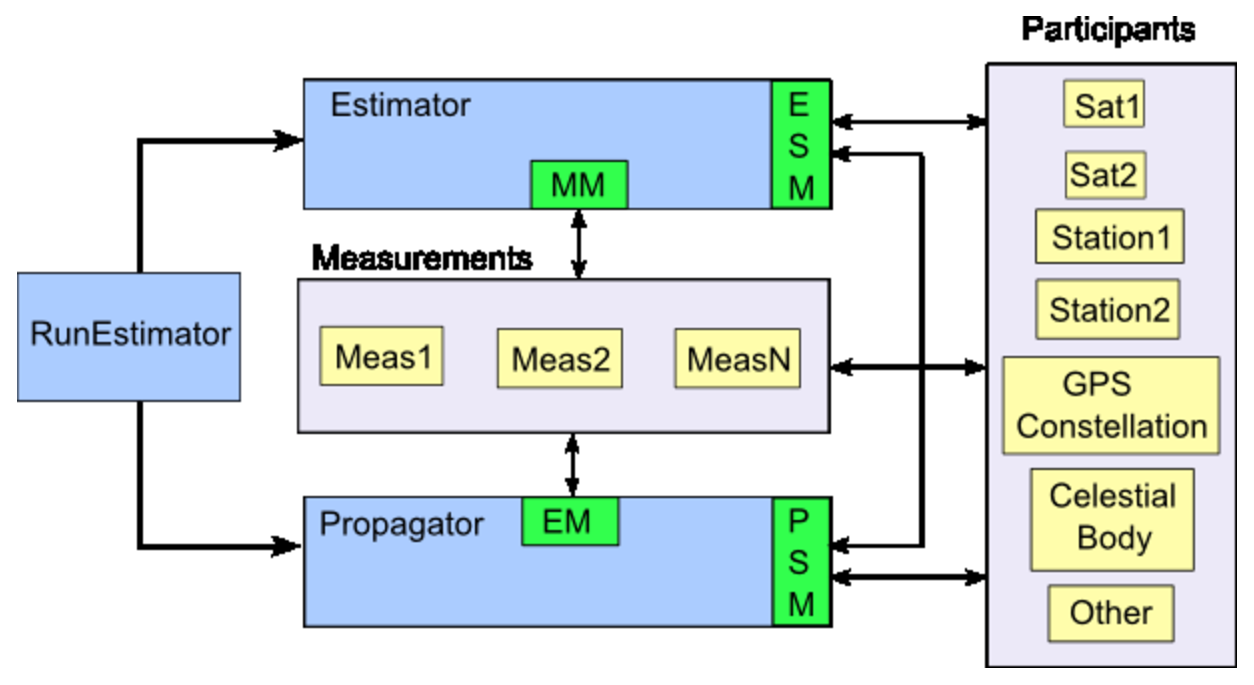
\includegraphics[scale=0.55]{Images/ODComponents.eps}
\caption{\label{fig:ODIneractions}OD Components and Interactions}
\end{center}
\end{figure}

\paragraph{Estimator -> ESM}  The ESM is an ``owned-object'' of an estimator.  The estimator
interacts with the ESM to get/set state related data from/on estimation participants.  The estimator
communicates with the ESM through several interfaces depending upon the type of state data such as
STM, covariance, or state vector.

\paragraph{ESM - >Participants}  The ESM communicates with participants to set and get state related
data.

\paragraph{Measurements->Participants}  Measurements communicate directly with measurement
participants/sensors.  Measurement objects have pointers to all measurement participants in the
measurement and therefore have direct access to public state data required to calculate measurement
values and partial derivatives.

\paragraph{PSM -> Participants}  The PSM communicates with participants to set and get state related
data.  This interface is similar to the ESM->Participants interface, except the PSM and ESM may not
manipulate the same state data.

\paragraph{ESM -> PSM}  The PSM and ESM interact during initialization.  The ESM provides the PSM
with a list of objects and IDs that are involved in the estimation process.  The PSM uses this
information to determine which states require propagation, and how those states should be propagated
(analytically or numerically).  In terms of the component level design, the PSM uses the data
provided by the ESM to generate the ListItem structure discussed in detail in the Component Design
section.

\paragraph{RunEstimator -> Propagator}  The RunEstimator command communicates with the propagator to
perform initialization and to propagate estimation participants.

\paragraph{RunEstimator -> Estimator}  The Estimator and the RunEstimator command function as a
finite state machine.  This is a complex interaction described in detail in later sections.

\paragraph{MM -> Measurements}  The measurement manager interacts with measurements during
initialization and execution.  During initialization, the measurement manager calls each measurement
object's Initialize() method and calls its GetObsData() method to get the arrays of epochs,
observations, and pointers to the measurement data objects.  During execution, the measurement
manager calls the Evaluate() and GetPartials() methods on the measurement object.

\paragraph{Estimator -> MeasurementManager}  The estimator interacts with the measurement manager to
get computed measurement values and partial derivatives and other measurement related information.

\section{Walkthrough of Sample Script Execution}

In this the remainder of this chapter, we present a simple estimation example in script form and
show at an intermediate level how GMAT would load and execute the script.  The first subsection
contains the sample script. The next subsection contains a general discussion of the steps GMAT uses
to execute any script.  We identify six key areas in the execution process that must be addressed in
the design of new estimation components and conclude the section with a more detailed discussion of
what happens for the new estimation components in those six key areas.  The design for the objects
used in this example are contained in the later chapters of this document.

\subsection{The Sample Script}

The sample script used for the execution walk-through has 5 objects:  a spacecraft named ODSat, a
ground station called Maui, a batch estimator called BLS, a measurement object named MauiData, a
propagator named ODprop, and a RunEstimator command.   The system processes range measurements
between Maui and ODsat using a batch least squares estimator.    The solve-for states are the
Cartesian states of the spacecraft.

\begin{quote}
\begin{verbatim}
%==========================================================================
%------  Define the spacecraft properties
%==========================================================================
Create Spacecraft ODSat;
ODSat.Id    = 21639;
ODSat.Epoch = 24228.72771990741;
ODSat.X     = 9882.164071524565;
ODSat.Y     = -23;
ODSat.Z     = 1837.579337039707;
ODSat.VX    = 0;
ODSat.VY    = 6.233189510799131;
ODSat.VZ    = 0.8480529946665489;
ODSat.OrbitCovariance = diag([100000^2*ones(3,1);1000^2*ones(3,1)]);

%==========================================================================
%==========================================================================
%------  Define the batch least squares solver
%==========================================================================
%==========================================================================
Create GroundStationMeasurement MauiData;
MauiData.Filename       = 'LEOMaui.mat';
MauiData.AddDataType = {'Range','ODSat','Maui'};

%==========================================================================
%------  Define the batch least squares solver
%==========================================================================
Create BatchEstimator BLS
BLS.MaxIterations   = 10;
BLS.RelTolerance    = 1e-5;
BLS.AbsTolerance    = 1e-5;
BLS.Measurements    = {'MauiData'};
BLS.SolveFor        = {'ODSat.CartesianState'};
BLS.Propagator      = 'ODProp';

%==========================================================================
%-----  Define the ground station properties
%==========================================================================
Create GroundStation Maui;
Maui.Id = 222;
Maui.X  = -4450.8;
Maui.Y  =  2676.1;
Maui.Z  = -3691.38 ;

%==========================================================================
%-----  Define the Propagator
%==========================================================================
Create ForceModel ODProp_ForceModel;
GMAT ODProp_ForceModel.CentralBody = Earth;
GMAT ODProp_ForceModel.PointMasses {Earth};

Create Propagator ODProp;
GMAT ODProp.FM = ODProp_ForceModel;
GMAT ODProp.Type = RungeKutta89;
GMAT ODProp.InitialStepSize = 60;
GMAT ODProp.Accuracy = 9.999999999999999e-12;

%==========================================================================
%-----  Solve the estimation problem
%==========================================================================
RunEstimator BLS;
\end{verbatim}
\end{quote}

\subsection{Overview of a GMAT Run}

\begin{figure}[htbp]
\begin{center}
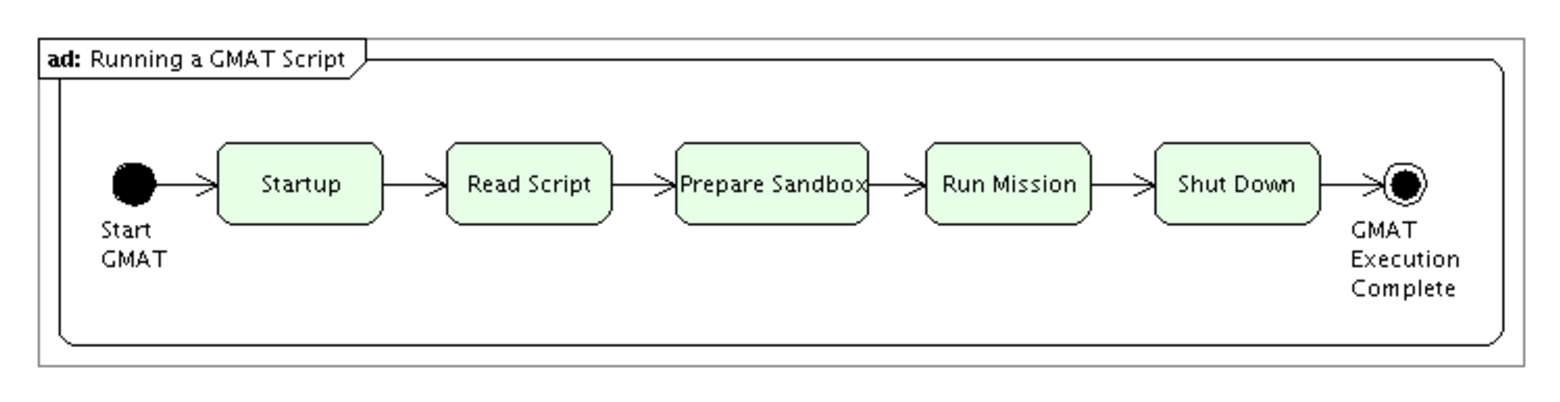
\includegraphics[scale=0.6]{Images/RunningaGMATScript.eps}
\caption{\label{fig:RunScript}GMAT Run Overview -- Running a Script}
\end{center}
\end{figure}

Figure~\ref{fig:RunScript} shows a high level view of the path through a run of a GMAT script.  When a user wants to run a GMAT script, she starts by opening the program, launching a set of actions that prepare the system for a run.  Once this startup process is complete, she loads the script into memory.  This script reading process creates the resources described in the script, loading them into GMAT's configuration (the container GMAT uses for objects created when building the resources in a script or from the GUI), and builds the commands in the Mission Control Sequence.  Next the objects are loaded into the Sandbox, and the Sandbox is prepared to perform the run by initializing all of the objects that were loaded.  The mission is run, executing the scripted sequence of commands. Finally, the user closes the program, completing the process.

\begin{figure}[htbp]
\begin{center}
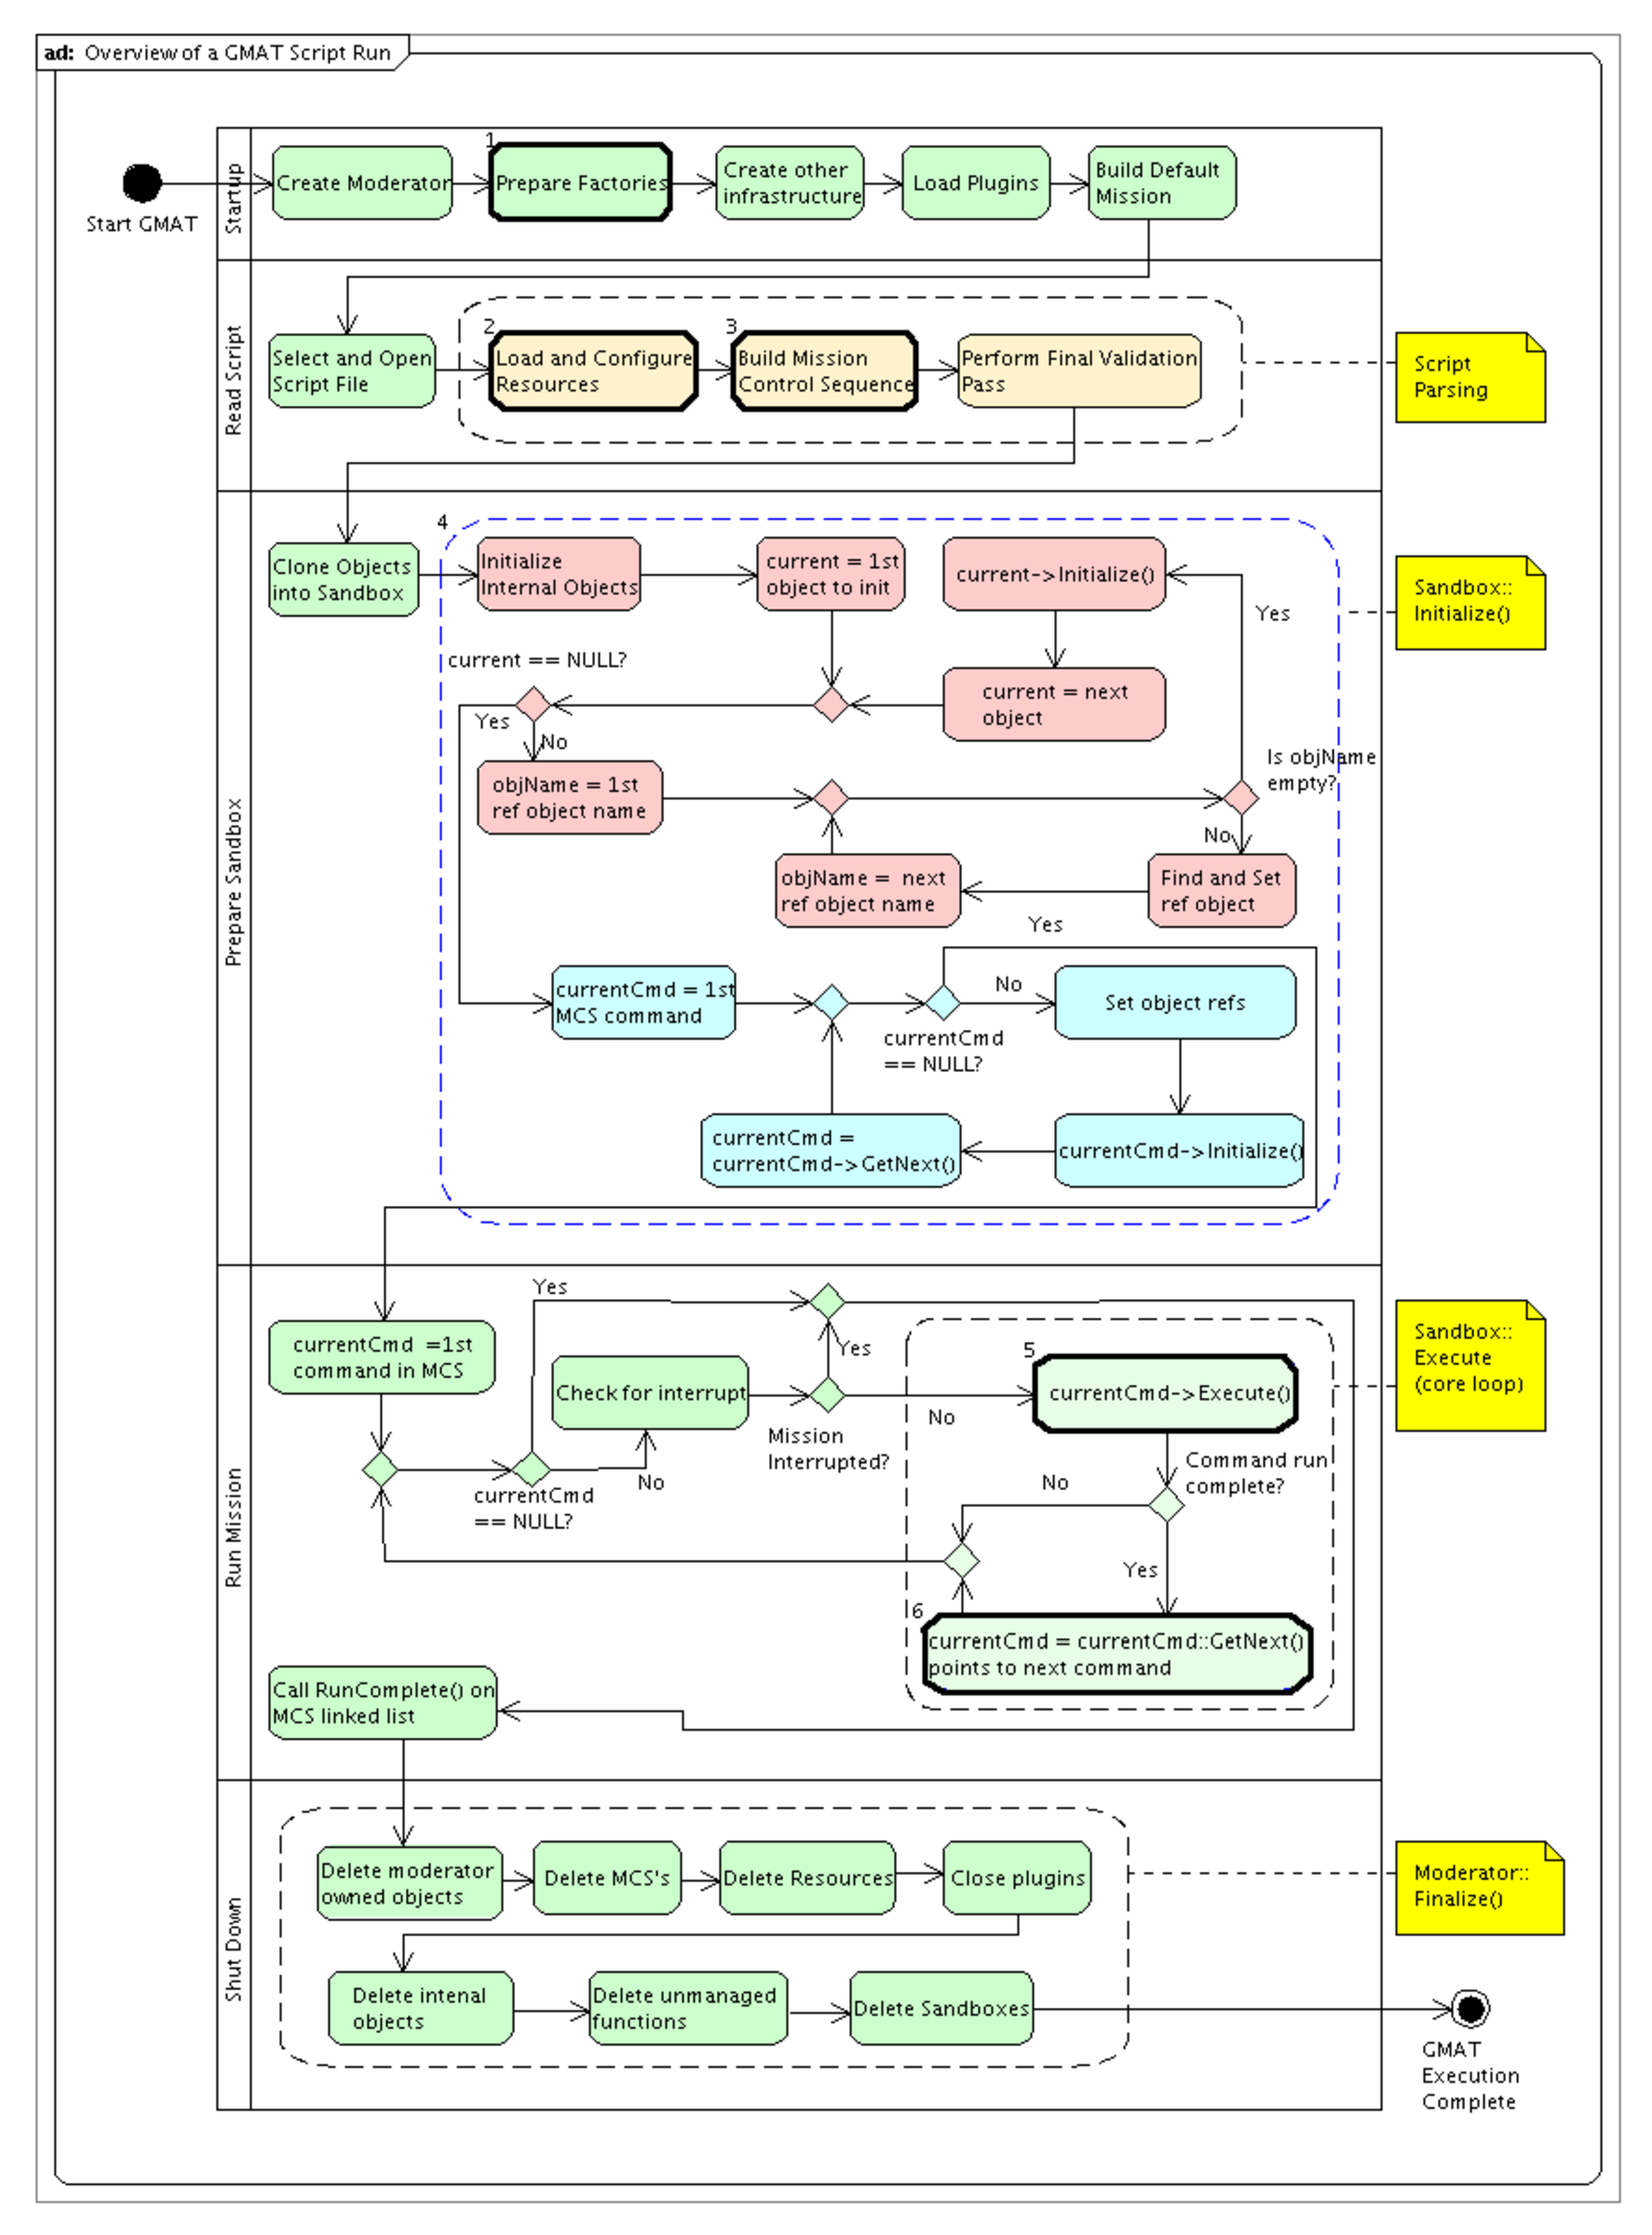
\includegraphics[scale=0.5]{Images/OverviewofaGMATScriptRun.eps}
\caption{\label{fig:RunScriptDetails}GMAT Run Overview -- Top Level Action Details}
\end{center}
\end{figure}

Figure~\ref{fig:RunScriptDetails} shows a first level expansion of these steps.  The details of the
steps shown in that figure can be found in the Architectural Specifications.  The blocks that are
affected by the new estimation components are numbered in the diagram, and will be discussed in more
detail in this document. There are six blocks that will be discussed here:

\begin{enumerate}
\item \textbf{Prepare Factories}  GMAT uses a set of components, called factories, to create
resources, commands for the Mission Control Sequence, and parameters used in calculations during a
mission run. New factories will be built to handle the new resources required to run estimation
problems in GMAT.
\item \textbf{Create and Configure Resources}  When GMAT parses a script, it reads the file one line
at a time, building the scripted objects and setting their parameters.  Depending on the resource,
the parameter setting phase may also include the creation and setting of objects owned by the
resource.
\item \textbf{Build Mission Control Sequence}  Following the resource definition and configuration
steps, the script describes the mission using a sequence of commands tailored to the components
supported by GMAT.  This sequence of commands is assembled into a linked list of objects called the
Mission Control Sequence.
\item \textbf{Prepare Sandbox}  GMAT runs missions inside of a component called the Sandbox.  When a
mission is run, the resources and Mission Control Sequence are loaded into the Sandbox used for the
run, interconnections between the components are established, and any pre-run data is set on these
components.  At the end of this process, the Sandbox is ready to execute the Mission Control
Sequence.
\item \textbf{Execute()}  Commands in the Mission Control Sequence manipulate the resources in the
Sandbox through a call to the Execute() method on each command in the sequence.
\item \textbf{GetNext()}  GMAT walks through the Mission Control Sequence by accessing the members
of the sequence's linked list.  Movement through the list is performed using the GetNext() method.
\end{enumerate}

These above six portions of a GMAT run are particularly relevant to the new estimation components.
The remaining blocks in the diagram may be discussed in passing, but the focus of the descriptions
necessary to build the pieces GMAT needs will include discussion of these six elements in more
detail.

The sample script presented earlier contains five resources and a command: a Spacecraft named ODSat,
a Measurement named MauiData (which contains two owned data members, a MeasurementReader and a
GroundstationRange MeasurementData object), a BatchEstimator named BLS, a GroundStation named Maui,
a Propagator named ODProp (with an owned ForceModel), and a RunEstimator command.  The estimator
contains a MeasurementManager and an EstimationStateManager as member objects.  Similarly, the
propagator contains instances of a PropagationStateManager and an EventLocator.  Each of the
following sections will conclude with a table reporting the status of GMAT and each of these six
objects after the process described in the section has acted on the sample script.  Prior to launch
of the system, the system description table looks like this:
\begin{center}
\begin{tabular}{|p{1in}|p{1.5in}|p{3in}|}
\hline\mc{3}{|l|}{\cellcolor[rgb]{0.75,0.75,0.75}\textbf{GMAT Status Before Starting the
Program}} \\
\hline\mc{3}{|p{5.5in}|}{The program has not yet started} \\
\hline\rowcolor[rgb]{0.9,0.9,0.9}\textbf{\textit{Object}} & \textbf{\textit{Status}} &
\textbf{\textit{Notes}} \\
\hline ODSat & Not yet created &  \\
\hline MauiData & Not yet created &  \\
\hline BLS & Not yet created & Once built, includes an EstimationStateManager and a
MeasurementManager as members \\
\hline Maui & Not yet created &  \\
\hline ODProp & Not yet created & Once built, includes a PropagationStateManager and an EventLocator
as members \\
\hline RunEstimator & Not yet created & \\
\hline
\end{tabular}
\end{center}

\subsection{Script Execution Walkthrough}

\subsubsection{Block 1: Prepare Factories}

GMAT's Factory subsystem is used to create all scriptable components of the system.  The subsystem
is an implementation of the Abstract Factory design pattern: it defines the interfaces used for
creating user objects and Mission Control Sequence commands, and uses derived Factory classes to
provide the implementation for specific class instantiations.  The Factory subsystem is managed by a
singleton instance of the FactoryManager class.  The Moderator calls methods on the FactoryManager
to create instances of specific types of objects, identified by the name of the object's type:
Spacecraft, GroundStation, DifferentialCorrector, and so forth.  Similarly, the Moderator calls the
FactoryManager to create instances of GMAT's command classes in order to build the Mission Control
Sequence.

Each Factory supporting user objects is registered with the FactoryManager when GMAT starts up.  The
internal factories are registered first, followed by factories contained in plug-in libraries.  The
addition of estimation capabilities to GMAT necessitates the construction of factories supporting
the new types of objects that are used for estimation, along with registration of these new
factories with the FactoryManager.  The ``Prepare Factories'' block of the master overview diagram
(Figure~\ref{fig:RunScriptDetails}) identifies the location of the factory registration in the life
cycle of a GMAT run.

Estimation requires the construction of five (check this) new factories for the internal
capabilities being designed here.  These new factories are:
\begin{itemize}
\item \textbf{EstimatorFactory}  The Factory that creates GMAT's internal estimators.  These
components could be added directly to the SolverFactory, since all Estimators are Solvers.  The
inclusion of a new factory for the Estimator objects keeps the factory subsystem more modular, and
will allow for inclusion of the estimation capabilities as a plug-in if desired.
\item \textbf{MeasurementFactory}  Measurement objects, a new class of object in GMAT, require a new
Factory supporting their instantiation.  The Measurement objects include elements that define data
types for the measurements and sources for observation data.  Separate factories are provided for
these elements.
\item \textbf{MeasurementDataFactory}  Creates the measurement data objects.  The measurement data
objects are used to calculate the expected value of a specific type of measurement along with the
partial derivatives associated with that value.
\item \textbf{ObservationReaderFactory}  Creates the objects used to read and write observation
data.  The observation data may be fed into GMAT from a data file, a database, or by means of a live
data feed.  The initial builds of GMAT's estimation subsystem are designed to work using data from a
file.
\item \textbf{EstimationCommandFactory}  Creates the commands used in estimation. The inclusion of a
new factory for the estimation commands objects keeps the factory subsystem more modular, and will
allow for inclusion of the estimation capabilities as a plug-in if desired.
\end{itemize}

The Moderator creates these factories during system start\footnote{Internal and plug-in factories
are constructed and registered in the Moderator's initialization code.  The Estimation
 code is built as a plug-in module, and as such, is loaded into the system by loading the library
at run time after all of the internal Factory objects have been loaded.}.  Each factory is passed
to the FactoryManager once it is created. The FactoryManager obtains the base type of the objects
supported by the factory along with a list of the supported types.  For example, in the initial
estimation release, the MeasurementDataFactory will report that it supports the
Gmat::MEASUREMENT\_DATA type, and can supply specific objects for ``GroundStationRange'',
``GroundStationRangeRate'', ``GroundStationRADec'', and ``GroundStationAzEl'' measurement data.

The factories identified above will be described in more detail in the class descriptions.  These
factories follow the same pattern as is found in the rest of GMAT.  There are no special
considerations imposed on the system by the inclusion of the estimation related factories.

Several new base object types will be added to GMAT to support estimation.  Specifically, new types
will be added to support Measurement classes, MeasurementData classes, and ObservationReader
classes.  (The Estimator classes are already handled through inheritance from the Solver base
class.)  The Factory base class and Gmat namespace will be extended to include these new types.

The following table shows the configuration of GMAT and the state of each of the objects contained
in the sample script after the factory registration phase is complete.

\begin{center}
\begin{tabular}{|p{1in}|p{1.5in}|p{3in}|}
\hline\mc{3}{|l|}{\cellcolor[rgb]{0.75,0.75,0.75}\textbf{GMAT Status After Preparing Factories}} \\
\hline\mc{3}{|p{5.5in}|}{This step prepares the elements of GMAT's engine that are needed to build
the resources and commands in a GMAT script.  All of the factories have been created and registered
with GMAT's FactoryManager.  GMAT is essentially idle, waiting for a user prompt to begin
processing.  The GUI versions of GMAT complete the system startup by building the default mission.}
\\
\hline\rowcolor[rgb]{0.9,0.9,0.9}\textbf{\textit{Object}} & \textbf{\textit{Status}} &
\textbf{\textit{Notes}} \\
\hline ODSat & Not yet created &  \\
\hline MauiData & Not yet created &  \\
\hline BLS & Not yet created & \\
\hline Maui & Not yet created &  \\
\hline ODProp & Not yet created & \\
\hline RunEstimator & Not yet created & \\
\hline
\end{tabular}
\end{center}

\subsubsection{Block 2: Load and Configure Resources}

The objects users configure in GMAT fall into two categories: Resources and Commands.  The elements
that define the time ordered sequence of actions in the Mission Control Sequence fall into the
latter category, and are discussed in the Block 3 description below.  The elements that identify the
physical objects and tools that manipulate those objects are called resources.  These components
include the Spacecraft; Groundstations; hardware elements (tanks and thrusters); celestial bodies
and special locations in the solar system; variables, arrays, and strings; targeters, optimizers,
and estimators; and other elements that act as items used when defining the mission timeline.  In
the GUI versions of GMAT, these pieces are located on the Resources tree, while the commands appear
on the Mission tree.

GMAT's script processing subsystem operates in two distinct modes: object mode and command mode.
The resources are created and configured in object mode, prior to the definition of the Mission
Control Sequence.  As soon as a command for the Mission Control Sequence is encountered, the
ScriptInterpreter changes from object mode into command mode.  Each subsequent line of the script
file is treated as a node in the control sequence, and placed into the linked list defining the
Mission Control Sequence.

Block 2 in the master overview diagram represents the actions taken by the ScriptInterpreter in
object mode.  In this mode, GMAT creates resources, saves them for later use, and sets parameters on
created resources.  Resources are built from script lines that start with the GMAT keyword
``Create''. When the ScriptInterpreter finds a line starting with that keyword, it takes the next
word in the line as the text describing the type of object requested, and the remaining words as the
names of objects of the specified type that need to be constructed.  The ScriptInterpreter passes
the request for each new object to the Moderator, which passes the request into GMAT's
FactoryManager.  The FactoryManager locates the factory responsible for creating the requested
object type, and passes the creation request into that factory.  The factory creates the requested
object, assigning it the specified name, and returns the new object's pointer to the Moderator.  (If
no object was created, the returned pointer is NULL.)  The Moderator passes the object into the
ConfigurationManager so that the new object can be stored for later use (objects managed this way by
the ConfigurationManager are referred to as ``configured objects''), and then returns the pointer to
the ScriptInterpreter.

Assignment lines -- that is, lines of the form ``object.parameter = value'' -- encountered in object
mode make calls directly into the configured objects, setting values on those objects.  This
parameter setting identifies values used by the objects, sets the identities for references the
objects use, and in some instances sets up owned objects that the configured objects need.  If an
object uses a reference to another configured object, the name of the referenced object is stored as
a string in the object that uses the reference so that the object pointer can be set during
initialization in GMAT's Sandbox.  For example, when the script line ``BLS.Propagator = ODProp;'' is
parsed, the BLS estimator is sent the string 'ODProp'.  The BLS propagator stores that string name
for use during the ``Prepare Sandbox'' phase to identify the propagator object that the estimator
needs.

Most of the object parameter setting needed by the estimation resources fall into the category of
parameter values and references set by object name.  Discussions for this type of parsing will not
be presented in detail in this document for all of the estimation components.  The components that
use owned objects will contain information detailing the creation and configuration of those
objects.  In particular, the Measurement objects own MeasurementData objects and ObservationReader
objects in order to provide calculated and observed data and derivative information to the
estimation process.  The management of these elements will be discussed in the class descriptions
below.

\begin{center}
\begin{tabular}{|p{1in}|p{1.5in}|p{3in}|}
\hline\mc{3}{|l|}{\cellcolor[rgb]{0.75,0.75,0.75}\textbf{GMAT Status After Creating and Configuring
Resources}} \\
\hline\mc{3}{|p{5.5in}|}{The resources defined in the script have been created, and all of the
object properties defined for these resources have been set.  Internal (``owned'') objects defined
for the resources have been created and set on the resources.  The next script line that is read
describes the first command in the Mission Control Sequence.  It will toggle the ScriptInterpreter
out of object mode and into command mode.} \\
\hline\rowcolor[rgb]{0.9,0.9,0.9}\textbf{\textit{Object}} & \textbf{\textit{Status}} &
\textbf{\textit{Notes}} \\
\hline ODSat & Created, Properties Set, Uninitialized & Scripted data values have been set. \\
\hline MauiData & Created, Properties Set, Uninitialized & The owned ObservationReader and
GroundstationRange objects have also been created and passed to MauiData.  The file handle for the
ObservationReader has not yet been opened.  \\
\hline BLS & Created, Properties Set, Uninitialized & Scripted data values have been set.  The names
of reference objects are set.  The pointers to the reference objects are all NULL.  The BLS
MeasurementManager and EstimationStateManager are created as part of the estimator, but not
initialized.  The EstimationStateManager and MeasurementManager objects have been created as object
members.  Neither contains any data. \\
\hline Maui & Created, Properties Set, Uninitialized & Scripted data values have been set. \\
\hline ODProp & Created, Properties Set, Uninitialized & Scripted data values have been set.  The
ODProp PropagationStateManager and EventLocator have been created as part of the propagator, but not
yet initialized. \\
\hline RunEstimator & Not yet created & \\
\hline
\end{tabular}
\end{center}

\subsubsection{Block 3:  Build Mission Control Sequence}

Resources in GMAT are built by the ScriptInterpreter running in object mode.  As soon as GMAT finds
a Mission Control Sequence command in the script file, it toggles into command mode, and remains in
that mode until the script has been fully read.  Commands in GMAT can be interpreted in one of two
different ways.  Commands that are scripted using a simple series of strings with no specialized
elements follow this format:
\begin{quote}
commandKeyword [element1 ...]
\end{quote}

(The formatting here is that optional elements lie in square brackets, and ellipses indicate
additional pieces matching the one preceding the ellipses.  If a selection is necessary between
several options, the choices are separated by a vertical bar.)  Commands formatted this way can be
handled directly by the ScriptInterpreter.  Commands that have more specialized syntax override the
GmatCommand::InterpretAction() method and provide customized parsing for the line of text defining
the command.

The estimation commands planned for the initial releases of GMAT's new capabilities, RunEstimator
and RunSimulator, fall into the former category.  These commands are passed a single command
parameter and possibly a mode string defining the mode of operation.  Details about the syntax for
each of these commands can be found in the descriptions of the command classes, later in this
document.

\begin{center}
\begin{tabular}{|p{1in}|p{1.5in}|p{3in}|}
\hline\mc{3}{|l|}{\cellcolor[rgb]{0.75,0.75,0.75}\textbf{GMAT Status After Building the Mission
Control Sequence}} \\
\hline\mc{3}{|p{5.5in}|}{This step completes the script reading phase of the Interpreter's work.
All that remains is the final pass through the objects to validate a few settings and to ensure that
all of the objects needed to run actually do exist in the ConfigurationManager's object container.}
\\
\hline\rowcolor[rgb]{0.9,0.9,0.9}\textbf{\textit{Object}} & \textbf{\textit{Status}} &
\textbf{\textit{Notes}} \\
\hline ODSat & Created, Properties Set, Uninitialized &  \\
\hline MauiData & Created, Properties Set, Uninitialized &  \\
\hline BLS & Created, Properties Set, Uninitialized &  \\
\hline Maui & Created, Properties Set, Uninitialized &  \\
\hline ODProp & Created, Properties Set, Uninitialized &  \\
\hline RunEstimator & Created, Properties Set, Uninitialized & The referenced Estimator, ODProp, is
identified by name.  The pointer is not set. \\
\hline
\end{tabular}
\end{center}

\subsubsection{Block 4:  Prepare Sandbox}

GMAT runs scripts in an instance of a specialized container class called the Sandbox.  The process
of running a script is performed in two phases: Sandbox Initialization and Sandbox Execution.  The
initialization phase consists of four steps, shown in Figure~\ref{fig:SandboxInitialization}.

\begin{figure}[htbp]
\begin{center}
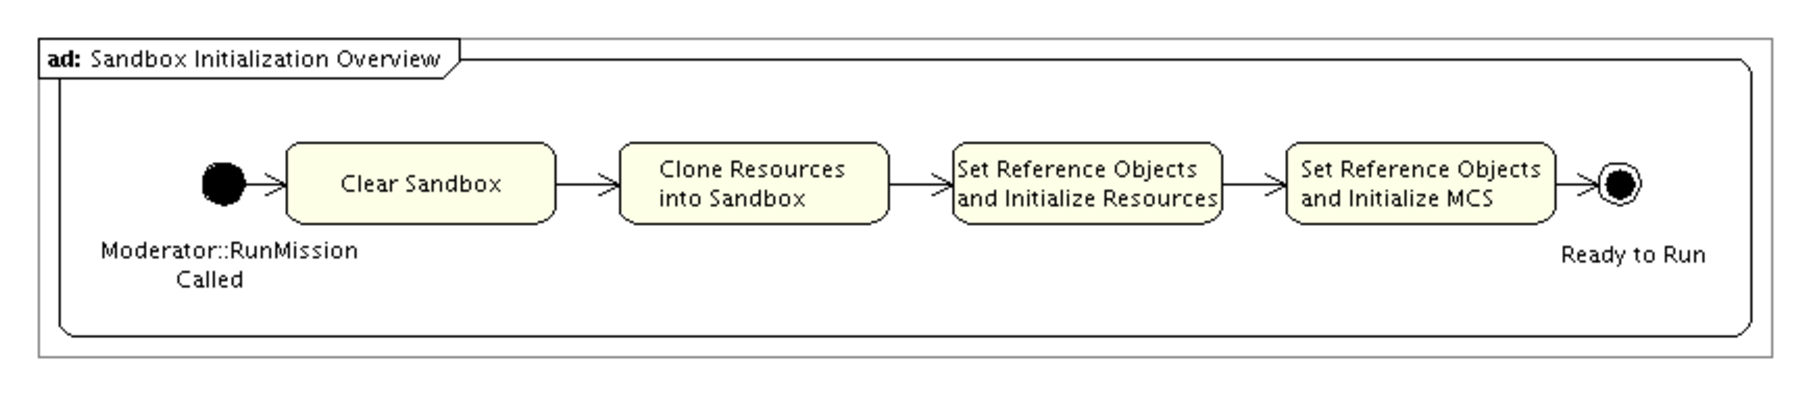
\includegraphics[scale=0.5]{Images/SandboxInitializationOverview.eps}
\caption{\label{fig:SandboxInitialization}Steps in the Sandbox Initialization Process}
\end{center}
\end{figure}

First, the Sandbox is instructed to clear its data structures in case there are objects in the Sandbox from a previous script execution.  Next, all of the resources managed by the
ConfigurationManager are copied into the Sandbox.  The original configured objects are not moved into the Sandbox; instead, the Sandbox makes a copy of each object for local use in the Sandbox, using each resource's Clone() method.  The Mission Control Sequence is also passed into the Sandbox at this time; the Mission Control Sequence is not cloned.

Once all of the resources have been cloned into the Sandbox, the Sandbox's Initialize() method is called.  This method initializes the resources and commands for use in the mission run.  The Sandbox performs this initialization of resources in an ordered fashion, ensuring that more basic resources are initialized before the components that use them are initialized\footnote{Resource initialization is actually handled in an instance of the ObjectInitializer class in the Sandbox.  The ObjectInitializer manages the ordered initialization process, which is performed as described here.}.  The resource initialization is performed one object at a time.  Resource initialization consists of three steps: (1) the Sandbox retrieves a list of objects referenced by the object that is being initialized, (2) each object in the list of references is located and passed by pointer to the object being initialized, and (3) the object's Initialize() method is called.

Steps (1) and (2) described here are illustrated in the system specifications\cite{archSpec}.  The Sandbox contains two object containers: the objectMap containing objects specific to the Mission Control Sequence but not automatically visible to functions in the control sequence, and the globalObjectMap containing objects visible to all commands in the Sandbox, including those in function calls.  This object scoping complexity is managed as part of the Sandbox initialization process.

\begin{figure}[htbp]
\begin{center}
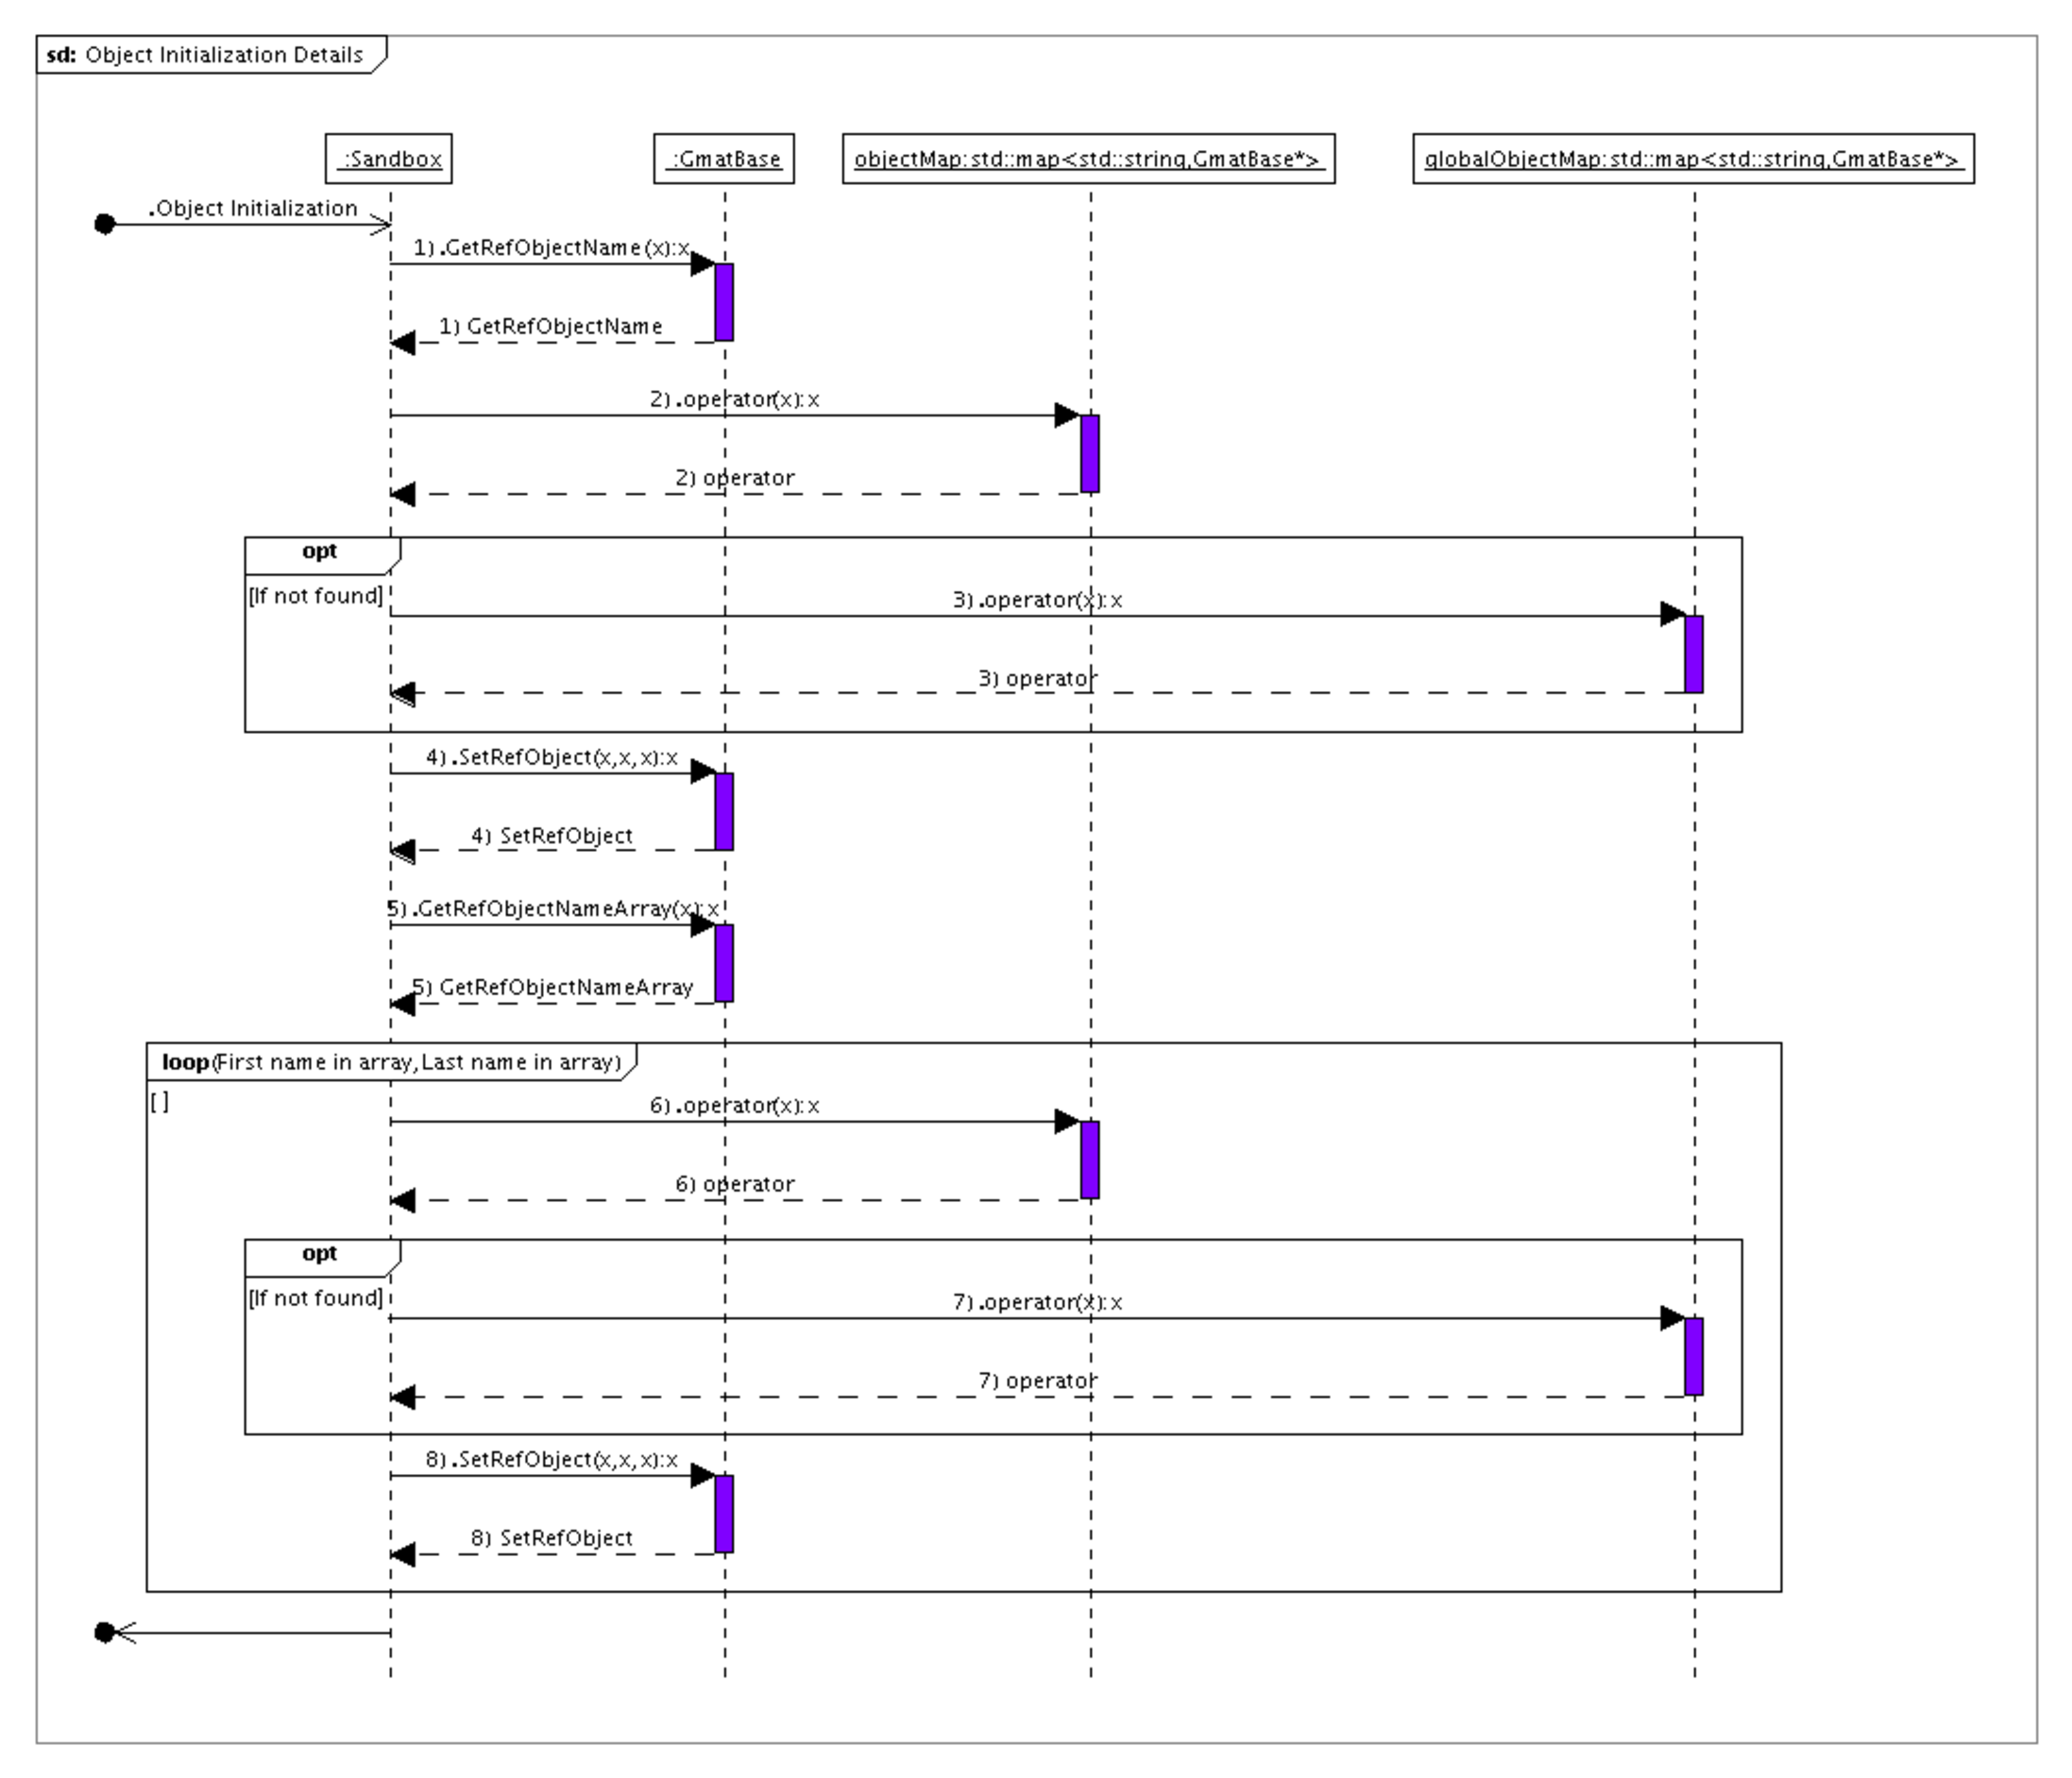
\includegraphics[scale=0.45]{Images/ObjectInitializationDetails.eps}
\caption{\label{fig:ObjectInitializationDetails}Reference Object Setting during Initialization}
\end{center}
\end{figure}

Objects in GMAT may contain object references that are accessed in one of two ways.  Objects with a single referenced object provide the Sandbox with the name of that object through a call to the GetRefObjectName() method.  Objects that reference multiple references provide a StringArray of reference objects names through a call to the GetRefObjectNameArray() method.  The calls made in the Sandbox to access these two methods are also shown in Figure~\ref{fig:ObjectInitializationDetails}.

After all of the resources have been initialized, the Sandbox initializes the Mission Control Sequence.  Control sequence initialization is performed one command at a time, using a pointer to the current command being initialized.  This process is performed in three steps.  First, the current command is passed a pointer to the solar system used in the Sandbox, the internal object pointers, and the arrays of the resources that were cloned into the Sandbox.  Once the command has these pointers set, it initializes itself through a call to its Initialize() method.  Finally, the current command pointer is updated to point to the next command that needs initialization through a call to the GetNext() method.

Sandbox initialization is the most complicated phase of a mission run in GMAT.  Because of this complexity, the initialization steps required for each of the new estimation objects will be described in the class descriptions below.

\begin{center}
\begin{tabular}{|p{1in}|p{1.5in}|p{3in}|}
\hline\mc{3}{|l|}{\cellcolor[rgb]{0.75,0.75,0.75}\textbf{GMAT Status After Preparing the Sandbox for the Run}} \\
\hline\mc{3}{|p{5.5in}|}{ Mission runtime copies of all resources and commands have been passed into the Sandbox.  Each resource has had its references to other resources set.  The Mission Control Sequence has been passed the local and global object stores (named objectMap and globalObjectMap in the code), and used these structures to locate and set pointers to the objects used by each command in the sequence.  GMAT is ready to run the mission. } \\
\hline\rowcolor[rgb]{0.9,0.9,0.9}\textbf{\textit{Object}} & \textbf{\textit{Status}} &
\textbf{\textit{Notes}} \\
\hline ODSat & Created and Initialized & All resources here are clones of the configuration
manager's objects.  Pointers to the referenced objects have all been set. \\
\hline MauiData & Created and Initialized &  \\
\hline BLS & Created and Initialized &  \\
\hline Maui & Created and Initialized &  \\
\hline ODProp & Created and Initialized &  \\
\hline RunEstimator & Created and Initialized & The pointer to the estimator has now been set. \\
\hline
\end{tabular}
\end{center}

\subsubsection{Block 5:  Execute() and Block 6:GetNext()}

Upon completion of the Prepare Sandbox step described above, all of the pointers connecting the objects together for the mission run have been set, and each element of the run has been given the opportunity to perform its initialization.  The commands in the Mission Control Sequence have all been passed pointers to the objects used to run the mission, and have been given the opportunity to perform their initialization.  The Mission Control Sequence is ready to run the mission.

\begin{figure}[htbp]
\begin{center}
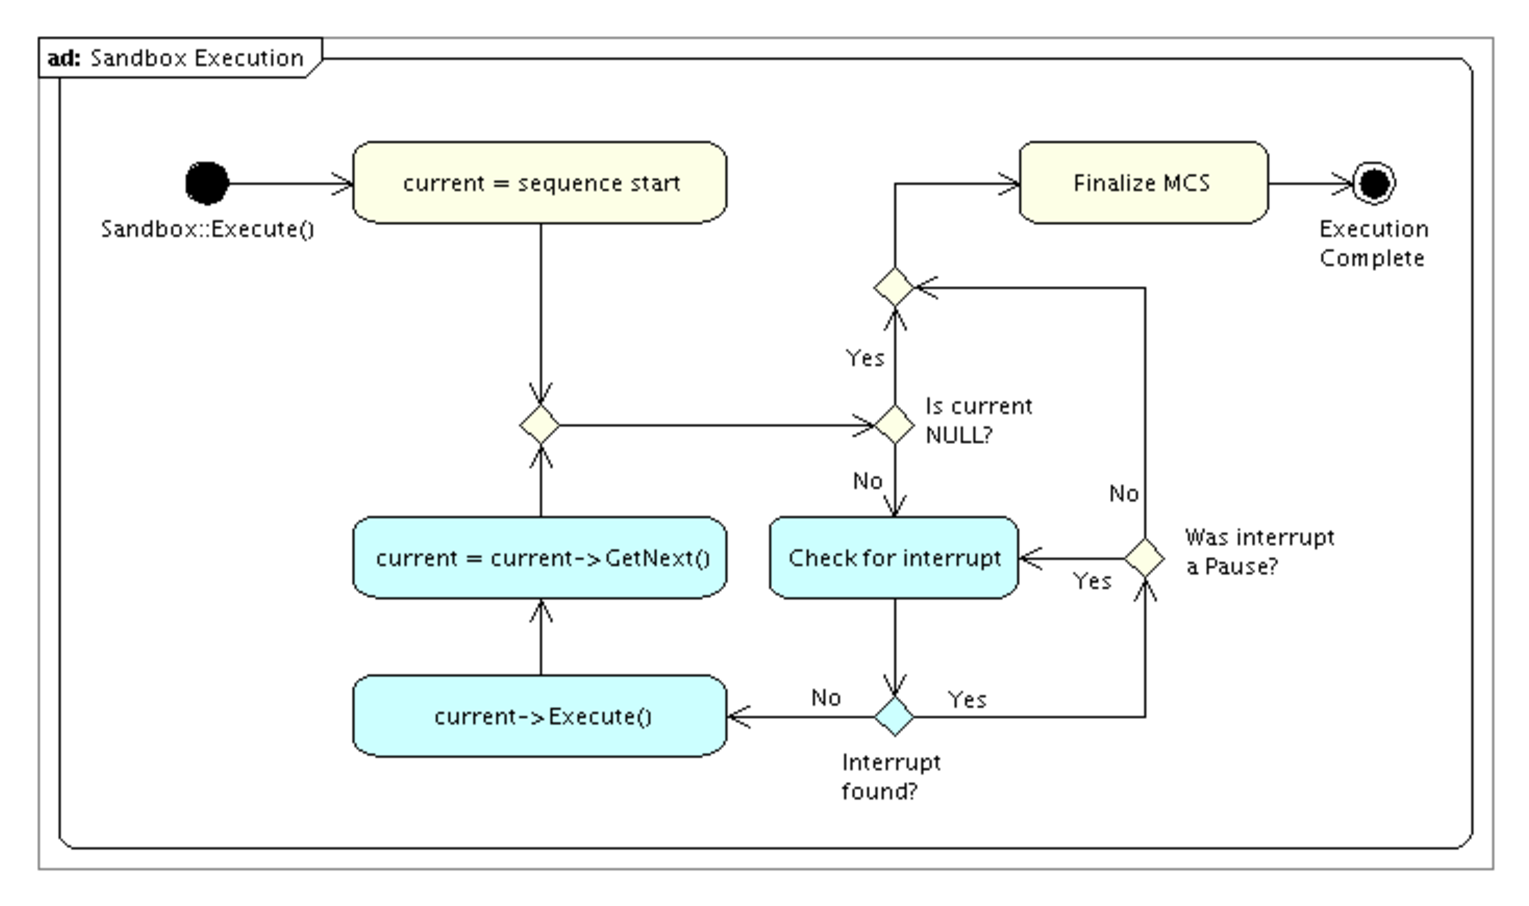
\includegraphics[scale=0.6]{Images/SandboxExecution.eps}
\caption{\label{fig:SandboxExecution}The Sandbox::Execute() Method}
\end{center}
\end{figure}

Figure~\ref{fig:SandboxExecution} shows the process GMAT follows when executing the Mission Control Sequence.  The Moderator launches the run through a call to the Sandbox's Execute() method.  That method sets a pointer to the first command in the Mission Control Sequence.  If that pointer is not
NULL, the Sandbox then places a callback to the Moderator to see if a user interrupt (typically a request to stop or pause the control sequence execution) has occurred.  If there is no interrupt, the command's Execute() method is called.  The command performs its processing, and returns control to the Sandbox.  The Sandbox then calls the command's GetNext() method, setting the command pointer to the next command that needs to be executed in the Mission Control Sequence.  If that pointer is not NULL, the Sandbox makes a callback to the Moderator to see if a user interrupt has occurred, and the process repeats. The run ends when the command pointer is set to NULL.  At that point, each command in the Mission Control Sequence is given the opportunity to finalize itself, and then control is returned to the Moderator, completing the run.

One subtlety in this process is the interplay between calls to a command's Execute() and GetNext() methods.  Some commands in GMAT -- particularly those that perform propagation and those that manage logical branching in the control sequence -- consume more computational time than desired before checking for user interrupts.  The implementation of the Execute() and GetNext() methods for these commands is designed to allow for interruption and reentry to the command so that interrupt checking can be performed while the command is executing.  At select times during execution of these commands, the process is paused and control is returned to the Sandbox.  The call to the GetNext() method in these cases returns a pointer to the executing command, rather than the next command in the Mission Control Sequence.  After the Sandbox performs the interrupt check, the command is called and execution resumes at the point where it was paused.

The commands that govern estimation -- specifically the RunEstimator, RunSimulator, and Estimate commands -- described in this document all exhibit this reentrant interrupt behavior.  The descriptions of those commands in the following sections include descriptions of this implementation in the descriptions of the execution process for the commands.

\begin{center}
\begin{tabular}{|p{1in}|p{1.5in}|p{3in}|}
\hline\mc{3}{|l|}{\cellcolor[rgb]{0.75,0.75,0.75}\textbf{GMAT Status After Calls to Execute() and
GetNext() are Complete}} \\
\hline\mc{3}{|p{5.5in}|}{GMAT has completed the run.  Each command in the Mission Control Sequence has been executed, with the possible exception of conditional branches that may have been skipped.  Command Summary data is available for each executed command.  The objects in the Sandbox have been used as dictated by the contents of the Mission Control Sequence.} \\
\hline\rowcolor[rgb]{0.9,0.9,0.9}\textbf{\textit{Object}} & \textbf{\textit{Status}} &
\textbf{\textit{Notes}} \\
\hline ODSat & Created and Exercised & Sandbox version of the ODSat object contains the results of
the estimation process \\
\hline MauiData & Created and Exercised &  \\
\hline BLS & Created and Exercised &  \\
\hline Maui & Created and Exercised &  \\
\hline ODProp & Created and Exercised &  \\
\hline RunEstimator & Executed Once & The command has been executed.  If the tracking data is
suitable, the estimator has run to completion and converged on a solution, which has been fed back into the resources in the Sandbox.\\
\hline
\end{tabular}
\end{center}


\part{Estimation Components}
\thispagestyle{empty}

\section{Estimators}

\subsection{Batch Least Squares}

\subsection{Extended Kalman Filter}


\chapter{Commands used in Estimation and Simulation}

\chapauthor{Stephen P. Hughes}{NASA/Goddard Space Flight Center}
\chapauthor{Darrel J. Conway}{Thinking Systems, Inc.}
\chapauthor{Matthew P. Wilkins}{Schafer Corporation}

GMAT's Solver subsystem uses a finite state machine model to drive the algorithms implanted in the solvers.  Each Solver object implements its own state machine, and pairs that state machine with a command or set of commands that manipulates GMAT's objects to provide data required for the algorithm.  The interaction between the solver and the command subsystem necessitates knowledge on the command side about the state information in the finite state machine.  In essence, the Solver finite state machine drives both the solver algorithm and a paired state machine implemented in the corresponding command.  The state and state transitions of the solution process is always controlled in the Solver object.  Object manipulations are performed in GMAT's Mission Control Sequence -- and in particular, in the Solver Control Sequence that uses the Solver object.

Each type of Solver is matched to command.  The targeters, like the differential corrector, are paired with the Target/EndTarget commands, and use the Vary and Achieve commands for additional communications needed by the targeting algorithms.  The optimizers are paired with GMAT's Optimize/EndOptimize commands, and use the Vary, Minimize, and NonlinearConstraint commands for communications.

There are four commands designed to pair with the estimation solvers: RunEstimator, RunSimulator, and (in the future) an Estimate/EndEstimate subsequence pair and a Simulate/EndSimulate subsequence pair.  This document describes the state machine activities for the first two commands. The subsequence based command pairs are not part of the first release of GMAT's estimation capabilities, and will be designed (along with any communications related commands) at a later date.

\section{Command Usage in GMAT}

Missions in GMAT are always executed by executing commands in a Mission Control Sequence.  The Mission Control Sequence is a linked list of command objects.  It is executed inside of one of GMAT's Sandboxes starting with the first node in the list, and progressing until the end of the list is executed.  The Sandbox drives this process when GMAT's Moderator calls the Sandbox's Execute() method.  The Sandbox tracks the executing command using a current command pointer, initially set to the first command in the list.

When the mission is run, the Sandbox checks for user interrupts, and then calls the Execute() method
on the current command pointer, executing that command.  Upon return from this call, the Sandbox
updates the current command pointer by calling the command's GetNext() method.  The pointer returned
from this call is then checked; if it is NULL, the Mission Control Sequence has run to completion.
If the returned pointer is not NULL, it points to the next command that needs to be executed, and
the process repeats by checking for interrupts and then calling the Execute() method on the command
pointed to by the current command pointer.  Thus overall control of the process running in GMAT's
Sandbox is managed by the commands in the Mission Control Sequence.

Some of the commands in the Mission Control Sequence manage their pointers to the next command in a reentrant fashion.  All of the commands that manage subsequences -- GMAT's ``branch commands'' -- work this way, as do the commands like Propagate that might take a long time to execute.  The call to GetNext() for these commands can return a pointer back to the command itself, rather than the next command in the list.  This self reference in the list transversal call (i.e. the call to ``GetNext()'') lets GMAT perform other processing during execution of time consuming commands.

\section{Estimation Command Overview}

\begin{figure}[htbp]
\begin{center}
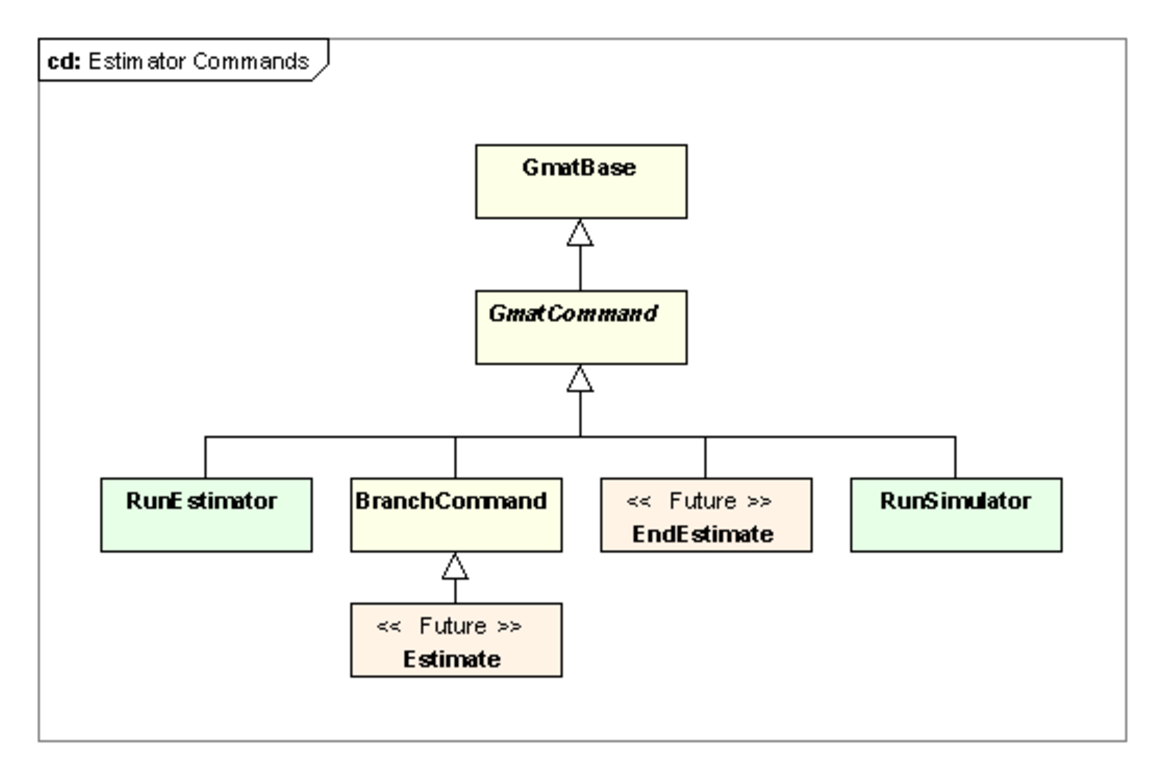
\includegraphics[scale=0.6]{Images/EstimatorCommands.eps}
\caption{\label{fig:EstimatorCommands}Commands Used in Estimation}
\end{center}
\end{figure}

The three command sets used for estimation -- RunEstimator, RunSimulator, Estimate/EndEstimate, and Simulate/EndSimulate, shown in Figure~\ref{fig:EstimatorCommands} -- all follow a similar methodology at the level of command execution. The commands interact with the estimator and simulator components to run the solver's finite state machine.  Each solver implements a state machine tailored to the needs of the implemented algorithm.

At the highest level, the state machine executes at prompting from the command, which in turn was prompted by a call from the Sandbox containing the Mission Control Sequence, as is shown in Figure~\ref{fig:EstimatorCommandCallSeq}. The estimation command is part of the Mission Control Sequence assigned to a Sandbox in GMAT.  When GMAT runs the Mission Control Sequence, it checks for user interrupts, and then calls the Execute method in the current command in the Mission Control Sequence.  The figure shows the high level flow that occurs for this process when the current command pointer is an estimation command, including the interactions between the command and the estimator.

\begin{figure}[htb]
\begin{center}
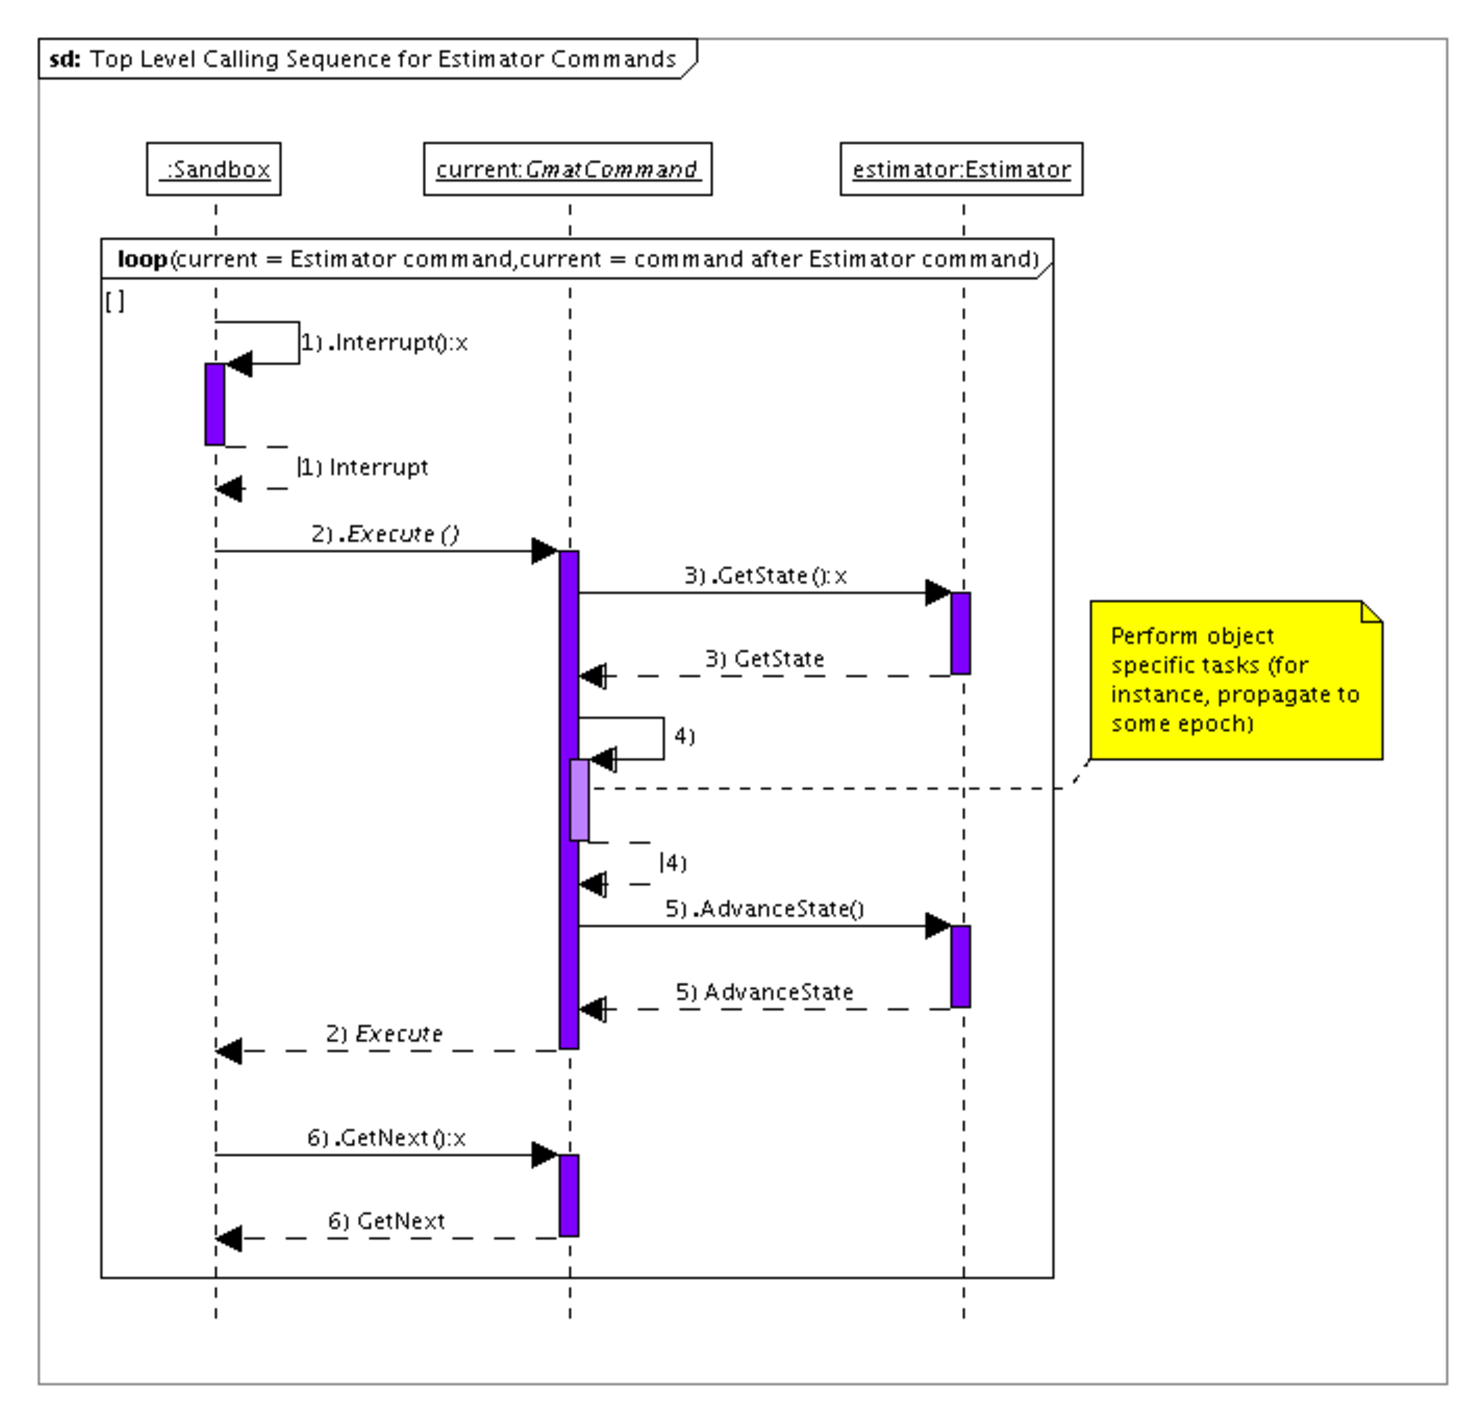
\includegraphics[scale=0.5]{Images/TopLevelCallingSequenceforEstimatorCommands.eps}
\caption{\label{fig:EstimatorCommandCallSeq}Top Level View of State Machine Execution}
\end{center}
\end{figure}

Each time the estimator command receives a call from the Sandbox to execute (made via the Execute() method), it queries the estimator for the current state, performs any requisite command actions based on that state, and then calls AdvanceState() on the solver so that the solver can perform the next action dictated by the state machine.  Upon return from the call to AdvanceState(), the command returns control to the Sandbox, which checks for user interrupts, and then calls the command's GetNext() method to determine the next command that needs to be executed.  The estimation command returns its pointer from this call as long as the solver's state machine is running.  The Execute() method is called on the command, which lets the estimation command process the next state in the state machine.  This sequence repeats until the estimation state machine runs the actions required by the FINISHED state, completing the estimation process.  Once the process has completed, a subsequent call to the command's Execute() method returns a reference to the next command in the Sandbox's Mission Control Sequence.

This general framework for estimation command execution in GMAT follows the basic execution framework for all GMAT commands: the Sandbox checks for interrupts, then executes the command, then retrieves the pointer to the next command to execute, and continues this process until the Mission Control Sequence is finished running.

This overview is intended to provide a framework for understanding the details of how the Estimation commands work in GMAT.  The following sections describe the estimation commands using the Batch Least Squares estimator to show the state machine elements of the design.  The state machine itself is described in the batch estimator section of this document.  The interactions required on the command side for the batch and sequential process are identical; from the point of view of the command, the process is to take an action, call AdvanceState() on the estimator, and repeat until the estimator reports that the process is complete.  We'll begin by examining the RunEstimator command.

\section{The RunEstimator Command}

The RunEstimator command drives the estimation process when the evolution of the participants can be modeled through propagation from one epoch to the next.  RunEstimator is a propagation-enabled command, meaning that it includes methods and data structures needed to perform propagation.  It supplies methods for performing actions in estimator state machines that support the following states:

\begin{itemize}
\item INITIALIZING
\item PROPAGATING
\item LOCATING
\item CALCULATING
\item ESTIMATING
\item CHECKINGRUN
\item FINISHED
\end{itemize}

The RunEstimator command provides methods that are called when the estimator's state machine is in one of these states and the Execute() command is called.  (The command's initialization is performed prior to the state machine call that detects the INITIALIZING state, so there is no need for a machine command function for that call.)  The command methods that perform actions based on the state of the estimator's state machine are listed here, and described in the command method description below.

\begin{itemize}
\item \textbf{INITIALIZING}:  Calls the PropagateToStart() method
\item \textbf{PROPAGATING}:  Calls to the Propagate() method
\item \textbf{LOCATING}:  Calls the PropToEvent() method
\item \textbf{CALCULATING}:  Calls the Calculate() method
\item \textbf{ESTIMATING}:  Calls the Estimate() method
\item \textbf{CHECKINGRUN}:  Calls the CheckConvergence() method
\item \textbf{FINISHED}:  Calls the Finalize() method
\end{itemize}

Different estimators can use different states in their state machines, and are likely to use the states in a different order based on the estimation algorithm.  For example, the batch least squares estimator does not use the ESTIMATING state until after all of the tracking data has been processed, while the sequential filters like the extended Kalman filter will estimate -- that is, advance through the ESTIMATING state -- as the data is processed.

Figure~\ref{fig:RunEstimatorStateMachine} shows the finite state machine for the batch least squares estimator (the lower portion of the sequence partition) and the RunEstimator command.  The core interaction supplied by the command during execution of the state machine for this example is the propagation of the participants in the estimation process.  The batch estimator performs the other steps of the estimation process without need for direct interaction with the command.

\begin{figure}[htb]
\begin{center}
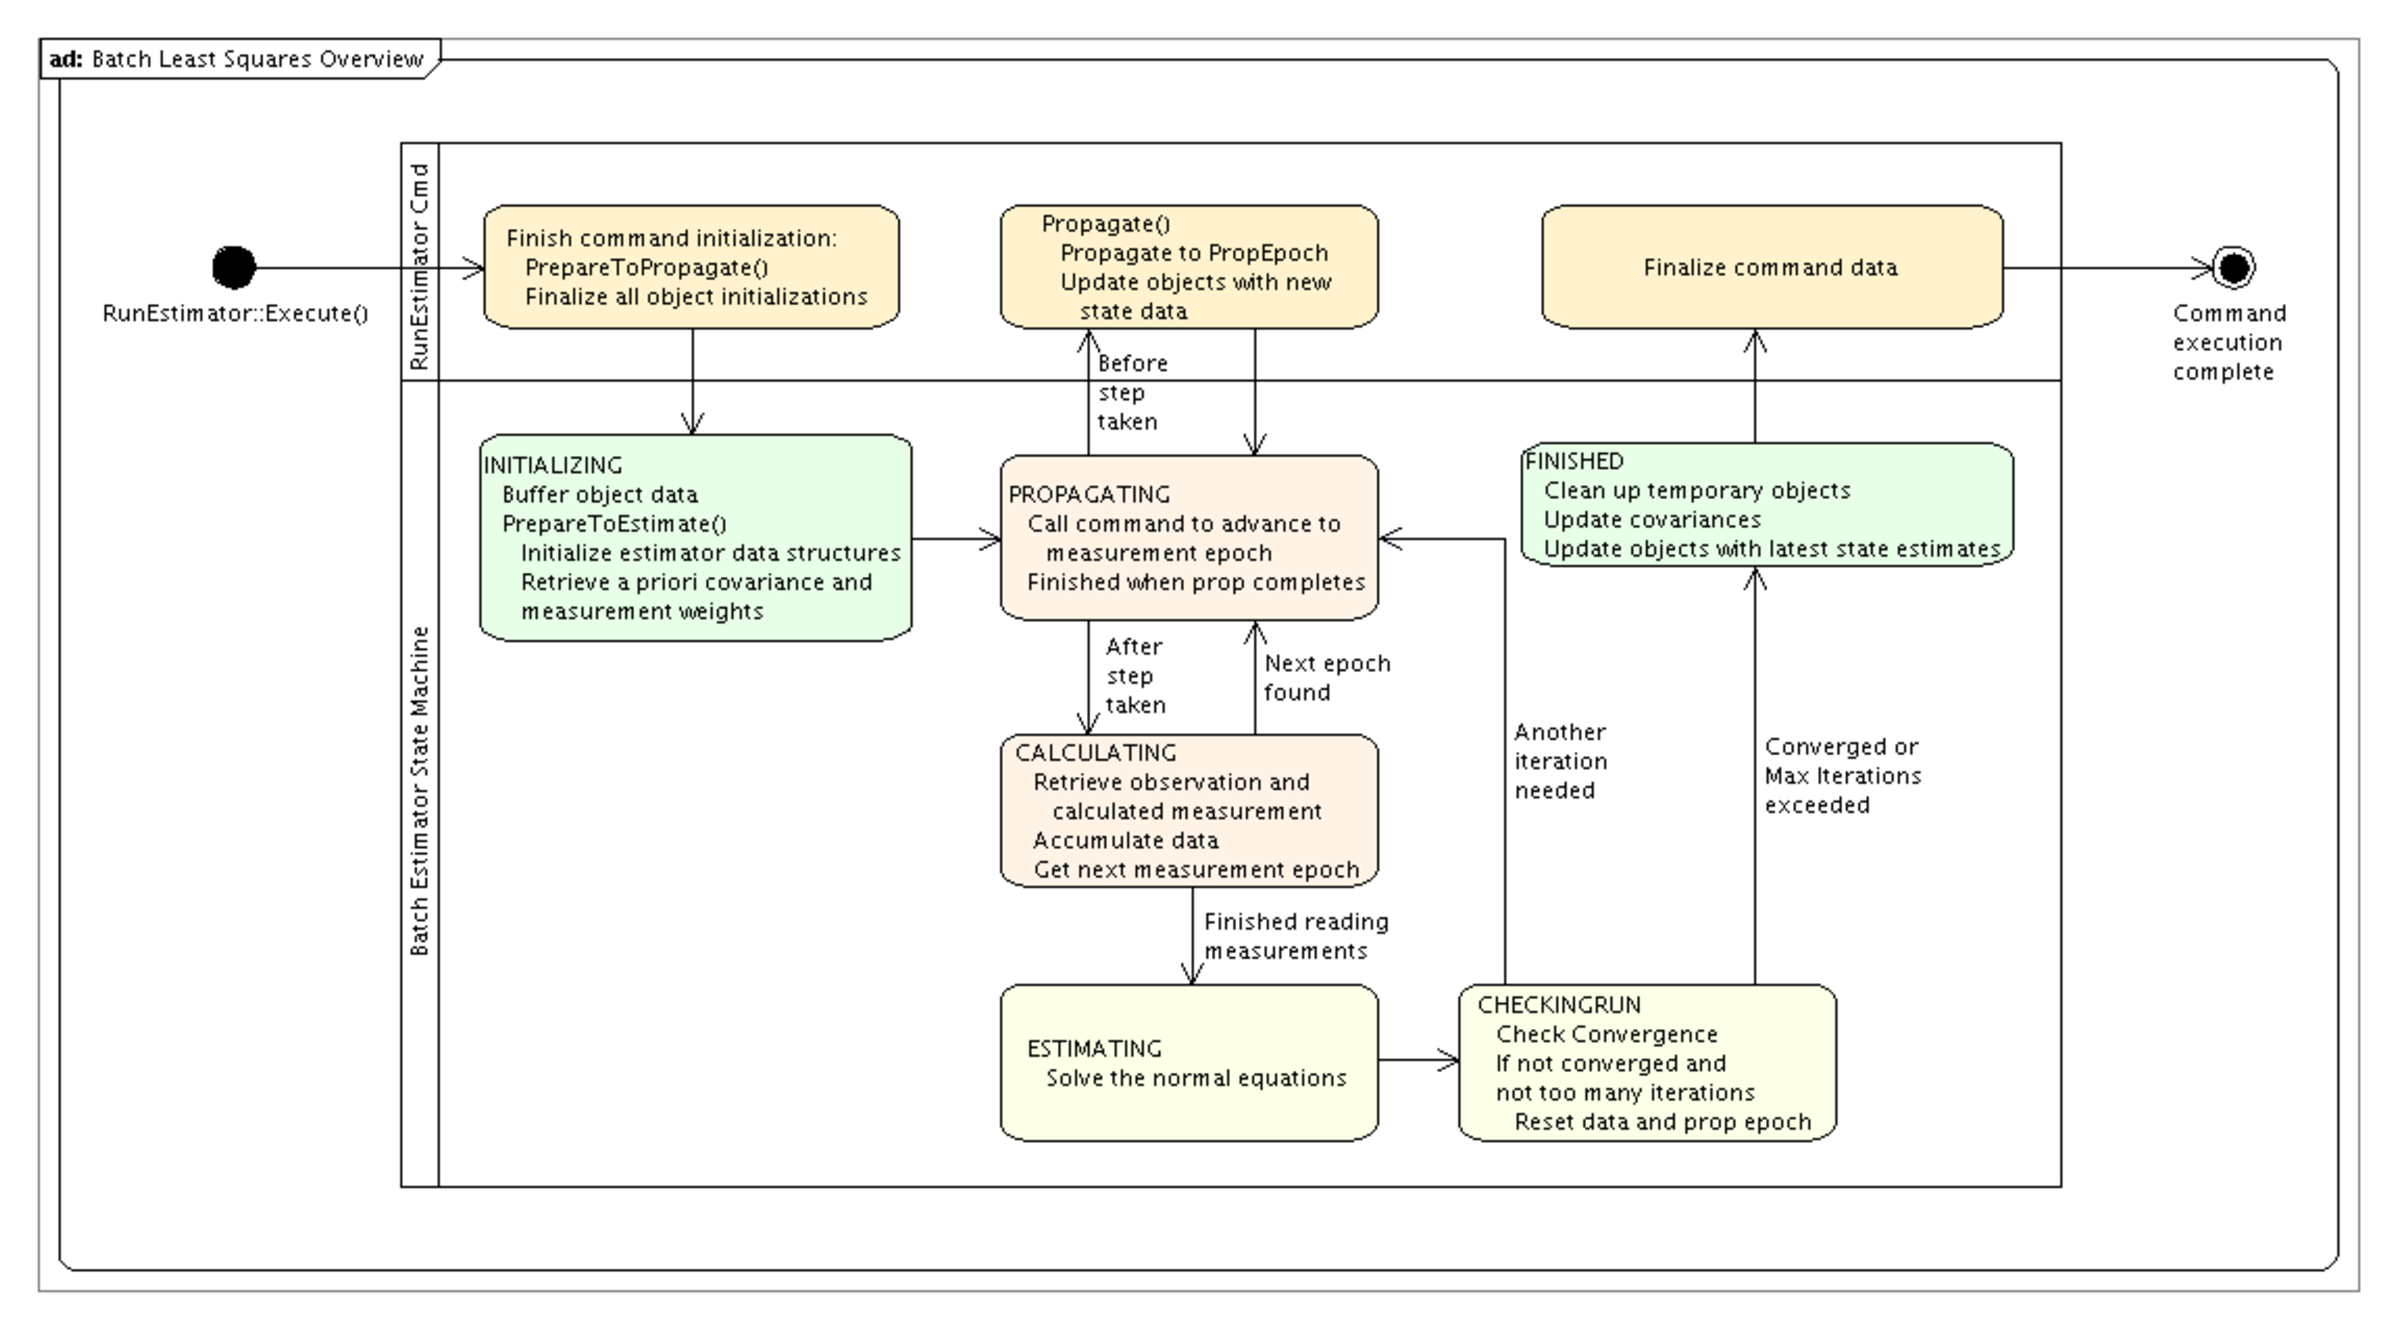
\includegraphics[scale=0.4]{Images/BatchLeastSquaresOverview.eps}
% BatchLeastSquaresOverview.png: 1134x621 pixel, 72dpi, 40.01x21.91 cm, bb=0 0 1134 621
\caption{\label{fig:RunEstimatorStateMachine}Interactions Between the RunEstimator Command and the Batch Least Squares Estimator}
\end{center}
\end{figure}

Three of the states specified here require propagation from the command.  The INITIALIZING state requires that the command perform propagation from the current state epoch to the estimation epoch specified on the estimator.  GMAT's objects are advanced from their current epoch to the next measurement epoch through calls to the Propagate() method, made when the finite state machine is in the PROPAGATING state.  Finally, event location to perform tasks like light-time corrections requires propagation.  These tasks are performed while the state machine is in the LOCATING state.

For each of these propagation steps, the RunEstimator command needs to know the size of the time step required to change from the current epoch to the desired epoch.  This information is retrieved from the estimator using the FindTimeStep() method.  The returned time step is then used to step the participants using a PropSetup reference in the command.  That reference, set during command initialization, points to the propagator owned by the estimator.  A future enhancement may allow the replacement of the estimator's propagator with a event-specific propagator tailored to the participants in the event calculation for propagation triggered from the LOCATING state.

The details of the state machine execution are described in the sections describing each specific estimator.  The description provided here is intended to specify the command actions required in the estimation process.

\subsection{RunEstimator Members}

The RunEstimator command contains the following data members and methods.

\paragraph{RunEstimator Attributes}

\begin{itemize}
\item \textbf{std::string estimatorName}:  The name of the Estimator that the command uses.
\item \textbf{Estimator *estimator}: A pointer to the Estimator.
\item \textbf{PropSetup *propagator}:  A pointer to the Propagator owned by the Estimator.
\end{itemize}

\paragraph{RunEstimator Methods}

\begin{itemize}
\item \textbf{virtual bool Initialize()}:  Sets internal references and interconnections, and prepares the estimator for use.
\item \textbf{virtual bool Execute()}:  Accesses the state from the finite state machine, performs any required command side actions, and then calls AdvanceState() on the estimator to move the finite state machine to its next state.
\item \textbf{virtual void PropagateToStart()}:  Queries the estimator for the time step required to propagate to the estimation epoch, and then performs that propagation.
\item \textbf{virtual void Propagate()}:  Queries the estimator for the next required time step, and then performs the required propagation.
\item \textbf{virtual void PropToEvent(bool restoreFromBuffer)}:  Queries the estimator for the time step estimated to find an event, and then performs the required propagation.  This method buffers the initial state data if restoreFromBuffer is false, and resets to that buffered data if restoreFromBuffer is true. A call to restore when the buffer has not been set results in an exception.
\item \textbf{virtual void Calculate()}:  Performs command side actions when the estimator is in the CALCULATING state.  This method is used to report intermediate data if the estimator text file is running in verbose mode.
\item \textbf{virtual void Estimate()}:  Performs command side actions when the estimator is in the ESTIMATING state.  This method is used to report intermediate data if the estimator text file is running in verbose mode.
\item \textbf{virtual void CheckConvergence()}:  Performs command side actions when the estimator is in the CHECKINGRUN state.  This method is used to report the status of the estimation process.
\item \textbf{virtual void Finalize()}:  Finalizes the command so that it can be reexecuted on a subsequent call. This method is also used to report the final estimated state and the status of the convergence criteria.
\end{itemize}

\section{The RunSimulator Command}

The RunSimulator command is a propagation-enabled command that manages the processes required to run and respond to the finite state machine defined in Simulator objects.  It supplies methods for performing actions in these state machines that when the finite state takes one of the following values:

\begin{itemize}
\item INITIALIZING
\item PROPAGATING
\item LOCATING
\item CALCULATING
\item SIMULATING
\item FINISHED
\end{itemize}

The RunSimulator command provides methods that are called when the simulator's state machine is in
one of these states and the Execute() command is called.  The command methods that perform actions
based on the state of the simulator's state machine are listed here, and described in the command
method description below.

\begin{itemize}
\item \textbf{INITIALIZING}:  Calls the PrepareToSimulate() method
\item \textbf{PROPAGATING}:  Calls to the Propagate() method
\item \textbf{LOCATING}:  Calls the PropToEvent() method
\item \textbf{CALCULATING}:  Calls the Calculate() method
\item \textbf{SIMULATING}:  Calls the Simulate() method
\item \textbf{FINISHED}:  Calls the Finalize() method
\end{itemize}

Figure~\ref{fig:RunSimulatorStateMachine} shows the finite state machine for the simulator in the lower portion of the sequence partition, and the non-trivial processes executed in the RunSimulator command.  The core interaction supplied by the command during execution of the simulator state machine is the propagation of the participants in the simulation process.  The simulator performs the other steps of the process without need for direct interaction with the command.

\begin{figure}[htbp]
\begin{center}
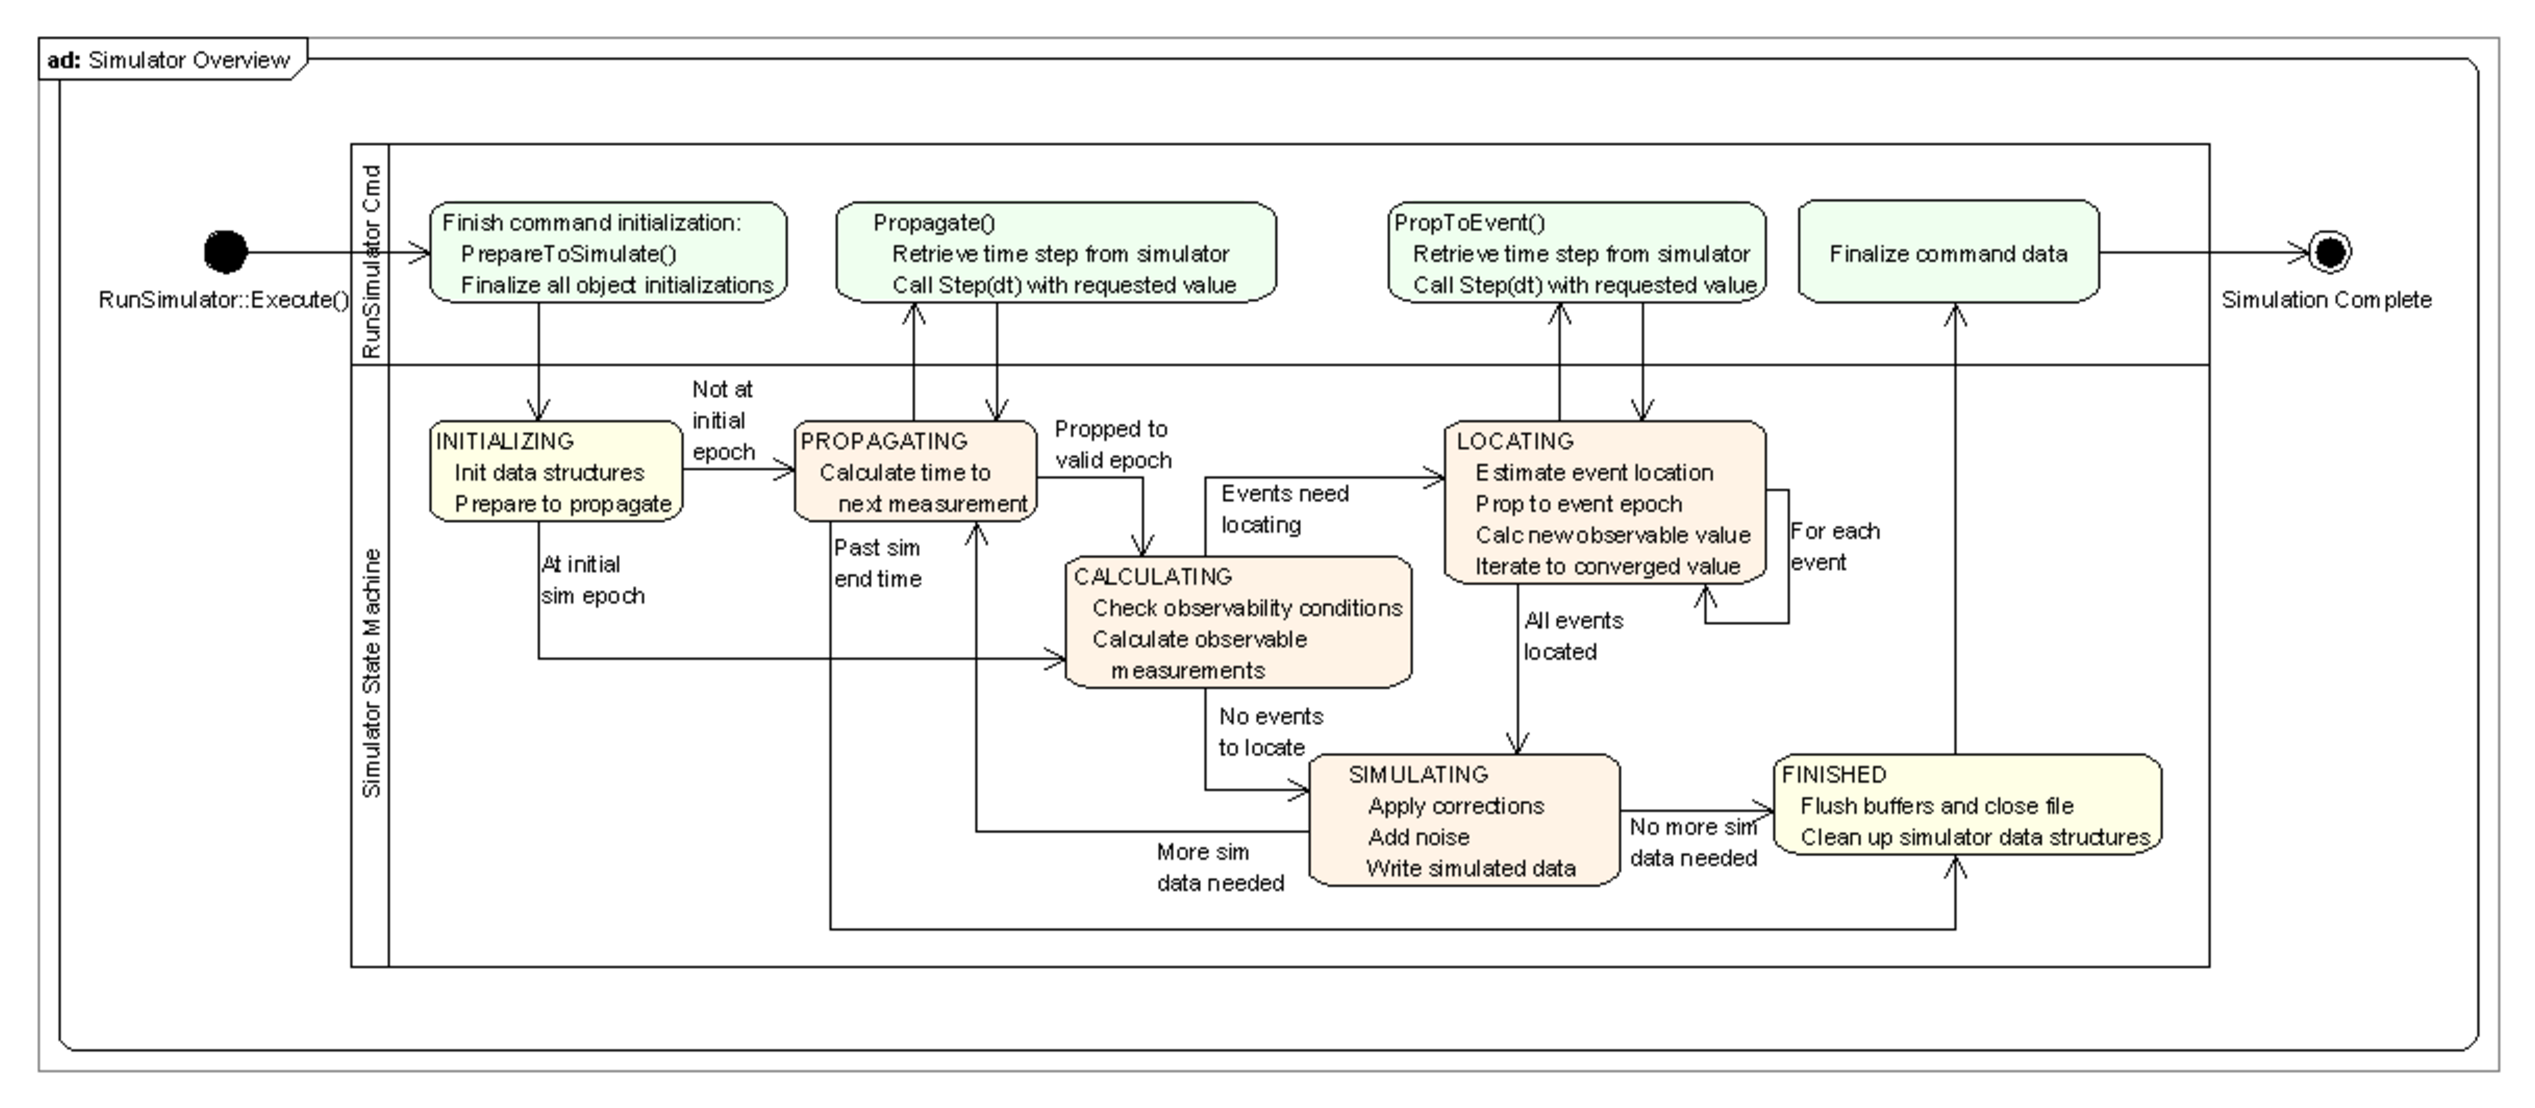
\includegraphics[scale=0.38]{Images/SimulatorOverview.eps}
% SimulatorOverview.png: 1201x516 pixel, 72dpi, 42.37x18.20 cm, bb=0 0 1201 516
\caption{\label{fig:RunSimulatorStateMachine}The Simulation State Machine}
\end{center}
\end{figure}

The RunSimulator command defines the interface between the Mission Control Sequence running in a Sandbox and a Simulator object.  The RunSimulator command manages all of the propagation performed in support of the simulation, simplifying the interrupt processing during the simulation.

In GMAT, the simulator object owns the propagator and the measurement manager.  The command retrieves the propagator pointer from the simulator for use during command execution.  The simulator also provides the information about the duration of any needed propagation to the command.  The RunSimulator command manages a buffer of objects that are propagated in support of the simulation, and uses this buffer to restore object data when performing calculations that would otherwise corrupt the time dependent states of those objects.  As an example, this object buffer is used during light time iterations so that the object states at the anchor time for a measurement can be restored after iteration has converged on the light time correction.

\subsection{Key Processes}

The RunSimulator command has two key processes, captured in the Initialize() and Execute() methods.

\subsubsection{Initialization}

The RunSimulator::Initialize() method performs the usual reference object location and setting tasks
performed by all commands.  For the RunSimulator command, this process involves finding the associated Simulator and cloning it for local use.  The Clone() process for a Simulator object includes a call that creates a clone of the propagator (a PropSetup object) used in the simulator.  The RunSimulator command retrieves a pointer to that clone for use when propagating elements of the simulation.  The command does not make an additional clone based on the simulator's propagator; it works directly with the propagator owned by the cloned simulator.

\subsubsection{Execution}

The RunSimulator::Execute() method determines the current state of the simulator's finite state machine, performs command side actions in response to that state, and then calls the simulator's AdvanceState() method so that the simulator can respond to the results of these actions.

Two specific states in the simulator use this interaction to trigger propagation: the PROPAGATING state is used to advance GMAT from one simulation epoch to another, and the LOCATING state is used to perform tuning of a simulated measurement through corrections that require propagation like light time iteration.  In both of these cases, the simulator is responsible for determining the size of the propagation steps that are necessary for the underlying process.  The RunSimulator command manages the actual evolution of the system based on the time step data retrieved from the simulator.

The propagation required in the LOCATING state requires buffering of information so that the objects in the simulation can be restored to their settings at the anchor epoch for the measurement.  The RunSimulator command determines when states should be buffered and reset through calls to the simulator.

\subsection{Class Design}

Figure~\ref{fig:RunSimulatorClass} shows the top level internal structure of the RunSimulator command.  RunSimulator is derived directly from the GMatCommand base class.  It references a Simulator object and, through that object, a PropSetup which provides the propagator infrastructure used by the command.

\begin{figure}[htbp]
\begin{center}
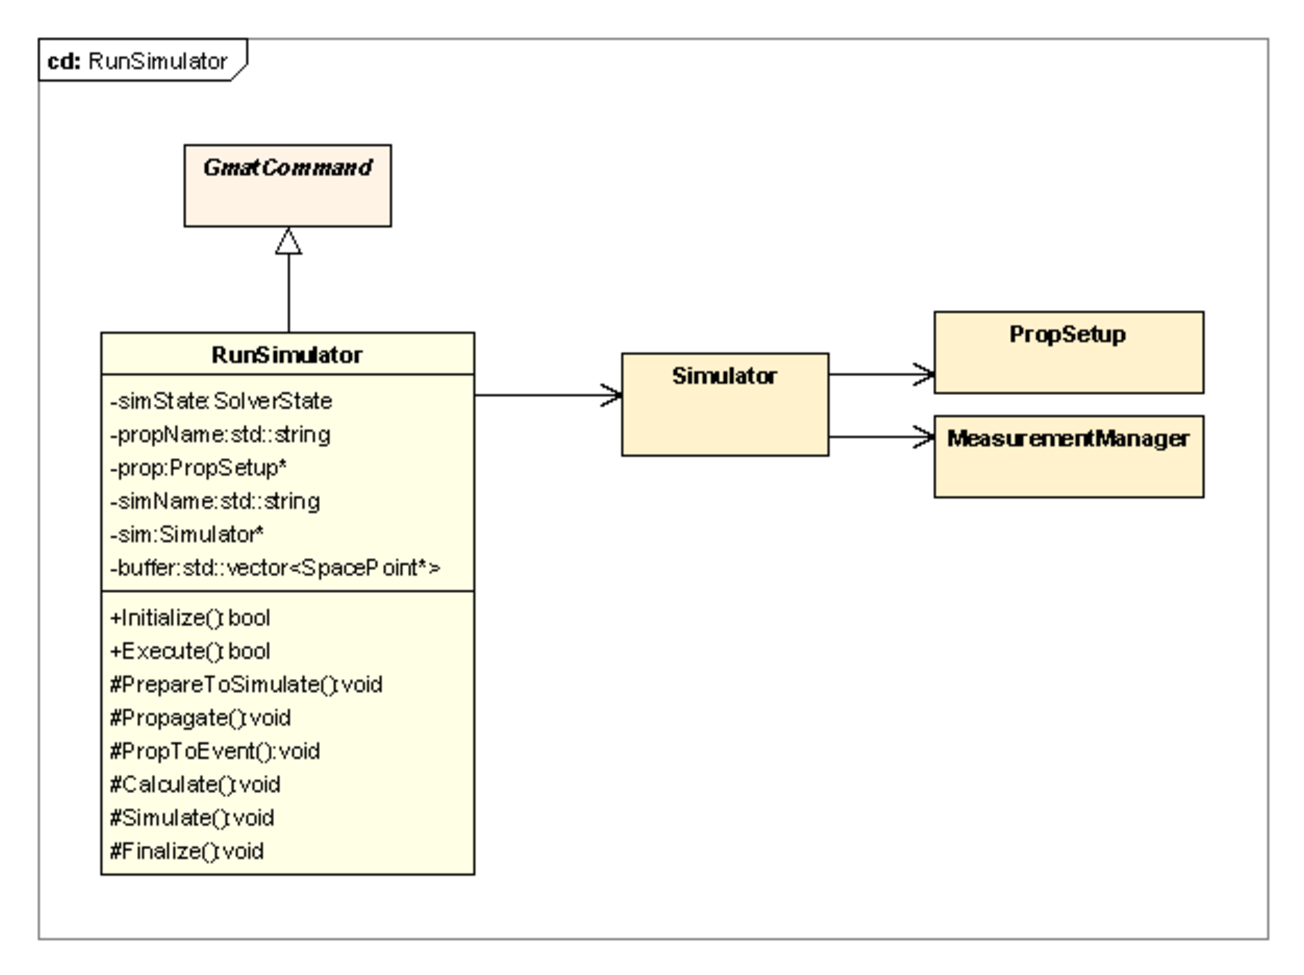
\includegraphics[scale=0.6]{Images/RunSimulator.eps}
% SimulatorOverview.png: 1201x516 pixel, 72dpi, 42.37x18.20 cm, bb=0 0 1201 516
\caption{\label{fig:RunSimulatorClass}The RunSimulator Class}
\end{center}
\end{figure}

\subsection{RunSimulator Members}

\paragraph{RunSimulator Attributes}

\begin{itemize}
\item \textbf{Gmat::SolverState simState}:  Tracks the state coming from the simulator's finite state machine so that appropriate actions can be triggered.
\item \textbf{std::string propName}:  Name of the PropSetup used to evolve the objects involved in the simulation.
\item \textbf{PropSetup *prop}:  A pointer to the simulator's copy of the configured PropSetup.
\item \textbf{std::string simName}:  The name of the simulator that implements the finite state machine.
\item \textbf{Simulator *sim}: A pointer to the simulator clone that is used with this command.
\item \textbf{std::vector<SpacePoint*> buffer}:  A local data buffer used to store copies of the simulation participants so that they can be restored later.
\end{itemize}

\paragraph{RunSimulator Methods}

\begin{itemize}
\item \textbf{virtual bool Initialize()}:  The method used to wire together all of components of the simulation that are available prior to execution of the Mission Control Sequence.
\item \textbf{virtual bool Execute()}:  The Mission Control Sequence entry point to the simulation.  This method makes calls to the AdvanceState() method on the simulator to drive the finite state machine.
\item \textbf{void PrepareToSimulate()}:  Method used to complete command initialization prior to execution of the finite state machine.  This method is triggered when the finite state machine is in the INITIALIZING state, prior to actual calls to the state machine.  The PropSetup completes initialization of its ODEModel and propagation state data during this call.
\item \textbf{void Propagate()}:  Propagates the components of the simulation when the finite state machine is in the PROPAGATING state.  This method queries the simulator for the desired time step (specified in seconds), and propagates by that duration to the next simulation epoch.  If the simulator specifies a zero time step, the command propagates by the natural time step of the propagator in the PropSetup.
\item \textbf{void PropToEvent()}:  Propagates the components of the simulation when the finite state machine is in the LOCATING state.  This method buffers the state data if necessary, queries the simulator for the desired time step (specified in seconds), and propagates by that duration to the next simulation epoch.  If the simulator specifies a zero time step, the command throws an exception and stops the simulation.
\item \textbf{void Calculate()}:  Method called when the finite state machine is in the CALCULATING state. This method is used to report status to the simulator text file.
\item \textbf{void Simulate()}:  Method called when the finite state machine is in the SIMULATING state. This method is used to report status to the simulator text file.
\item \textbf{void Finalize()}:  Cleans up the data structures used during the simulation, including the objects in the object buffer.  This method is triggered when the simulator is in the FINISHED state.
\end{itemize}


\chapter{\label{ch:EventLocation}Events and Event Location}

\chapauthor{Darrel J. Conway}{Thinking Systems, Inc.}

\section{Introduction}

GMAT provides a capability to determine precise epochs for important physical events along a modeled trajectory.  Examples of these events are shadow entry and exit, station rise and set, and other time-based quantities like the light time offset transmission and turn around of a tracking signal. Some of these quantities can be further processed to determine eclipse and station contact durations and similar time span quantities associated with detected event pairs.  GMAT's mathematical specification\cite{mathSpec} defines the event detection algorithm in some detail.  This chapter describes the software components that implement that algorithm.

\section{Components that Control Event Processing}

Event location in GMAT is controlled through interactions between five types of objects, and their interactions with the objects comprising the simulation designed by the user.  The five objects that work together to perform event location for these modelled objects are a propagation enabled command, a propagator contained in a PropSetup object, one or more Event objects, an EventManager, and a RootLocator.  These components play the following roles in the event location process:

\begin{itemize}
\item \textbf{Propagation Enabled Command}:  Provides the mission control sequence interfaces for event location.  Event locating is performed during execution of a propagation enabled command.  (Event evaluation can also be performed through parameter calculations tailored to report data from specific event objects.)
\item \textbf{PropSetup}:  Provides the propagator used to search for the event location.  Any GMAT propagator can be used in this context, including (once coded) ephemeris interpolators.
\item \textbf{Events}:  One or more objects responsible for providing calculations used to evaluate a measure of the desired event.  The Event objects all provide an Evaluate method that generates one or more Real values.  The values calculated in the Evaluate method are function values that evaluate to 0.0 at the epoch of the event, and that pass smoothly through zero as the data used in the evaluation are propagated through the time interval containing the event.
\item \textbf{Event Manager}: Acts as a mediator to control data interactions between the Event objects and the other components involved in the location process.
\item \textbf{Root Locator}: Manages the details of the propagation or interpolation needed to precisely locate the events on the mission timeline.
\end{itemize}

Event location is used in two distinct settings in GMAT.  During a typical mission run, users can script specific events that they would like to track for the purposes of reporting and analysis.  GMAT's propagation subsystem provides a mechanism to watch for these events as the mission is run, and locates the resulting events as they are encountered, tracking their location for the user.  Event location is also performed in the estimation subsystem, so that measurement corrections that require propagation to manage detailed precision calculation can find and propagate to the epochs for those events during the correction process.

GMAT manages two types of events: discrete events that occur at a single instant of time, and interval events that occur over a span of time.  In both cases, the epochs associated with the events are detected through zero crossings of a function.  Interval events track the start and end time for the event, and can be used to calculate the interval of time over which the event occurred.  For interval events, the event is deemed to be occurring while the event function provides a positive value.  Interval events that provide more than one Real value on event evaluation track the event span through the first event function evaluated; in other words, the first function value should be positive -- and all event criteria met -- while the interval event is happening.

This chapter presents the design for the former application.  Event processing during estimation follows the same process as generic event location, with a few additional steps required to synchronize the measurement models with the event location data.  The estimation based event location refinements are presented in Chapter~\ref{ch:MeasurementCorrections}.

\section{The Event Location Process}

Figure~\ref{fig:EventLocationSD} shows the details of the event location process.  Events that need to be located are registered with the propagation enabled command in the PrepareToPropagate() method prior to execution of the command.  At this point the EventManager evaluates each active Event and stores the event data so that the pre-propagation event state is known.  The propagation enabled command then takes a propagation step.  After the step has been taken, the EventManager again evaluates each event, and uses the results of that evaluation to determine if the event has a zero crossing or extremum in the propagation interval.  If no such trigger has occurred, the command continues processing -- either by taking additional propagation steps, or by exiting, returning control to the Sandbox so that the mission control sequence can continue executing.

\begin{figure}
\begin{center}
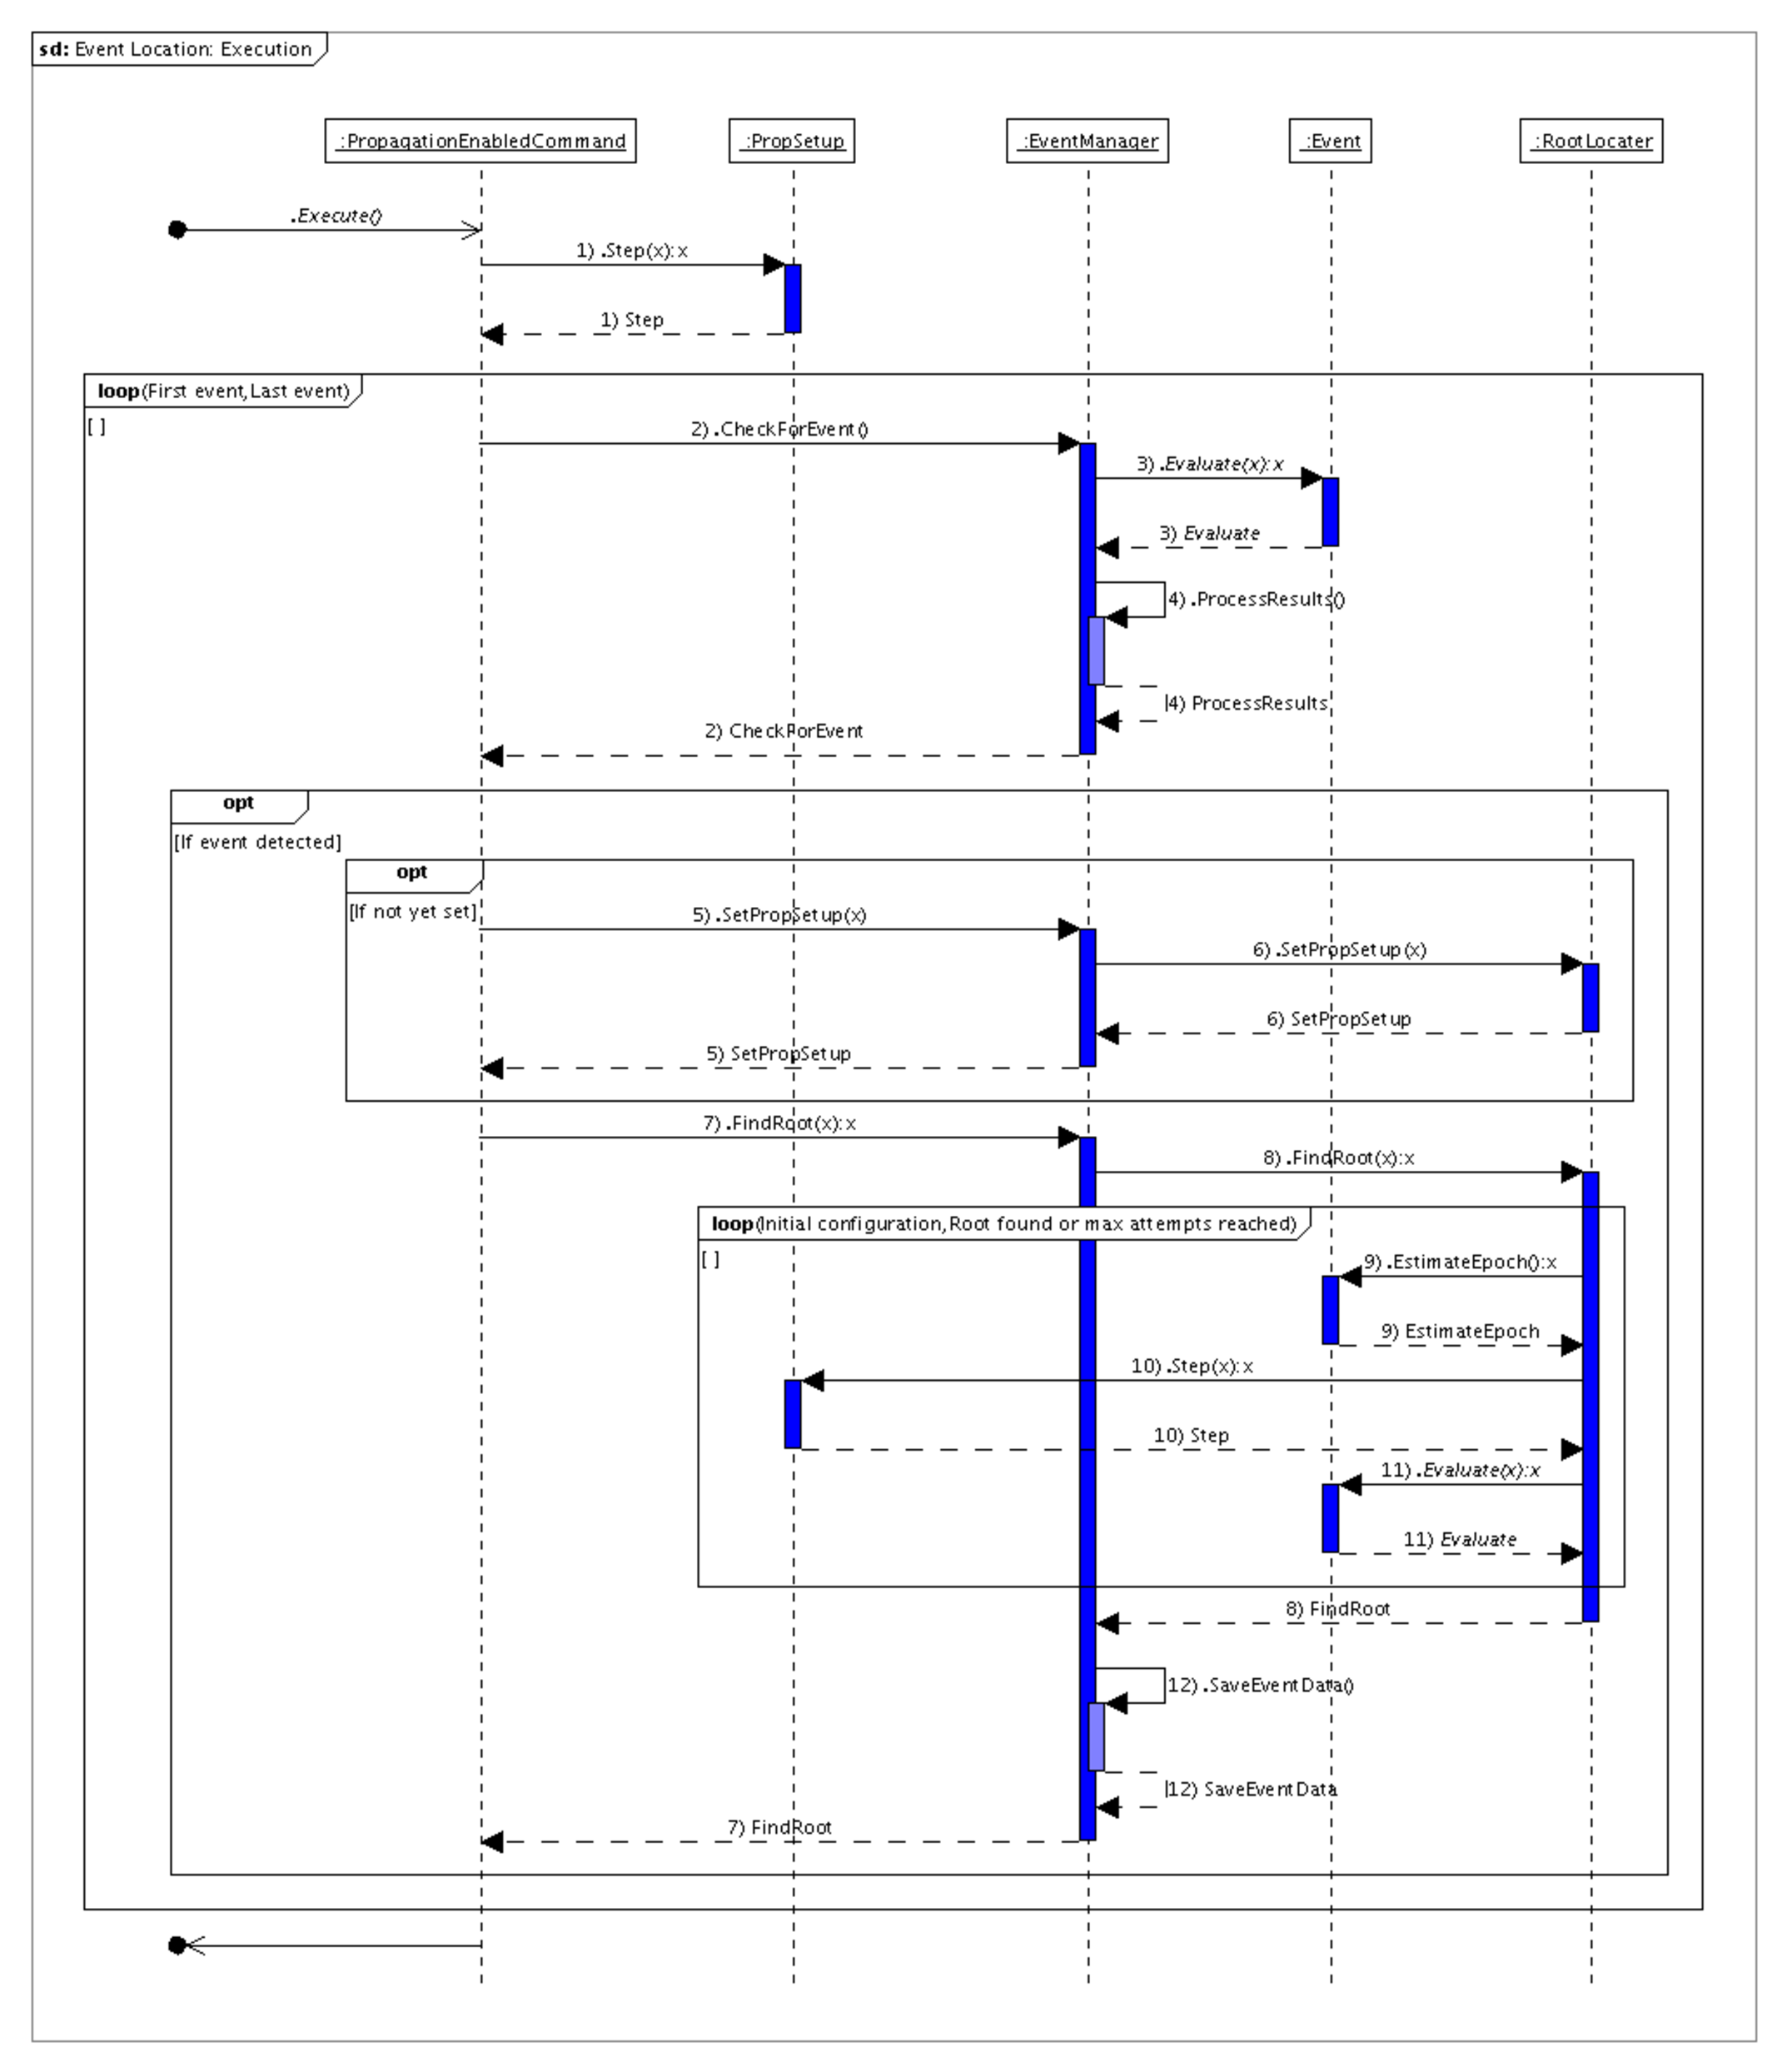
\includegraphics[scale=0.44]{Images/EventLocationExecution.eps}
% EventLocationExecution.png: 1014x1178 pixel, 72dpi, 35.77x41.56 cm, bb=0 0 1014 1178
\caption{\label{fig:EventLocationSD}The Event Location Process}
\end{center}
\end{figure}

If a zero crossing or extremum is detected in the propagation step, the event location code needs to perform additional processing.  This additional processing is controlled by a RootLocator object set during the command's initialization.  If necessary, the RootLocator is passed a pointer to the PropSetup associated with the located event\footnote{Some propagation enabled commands set the PropSetup pointer at initialization; for others, the PropSetup must be set at this point during execution.  The key differentiator for this determination is the relationship of the PropSetup to the other activities performed by the command.  Commands that only use a single PropSetup can set the pointer during initialization, while those that use multiple PropSetups must set the pointer at this point in the process.}.  Control is then handed to the RootLocator responsible for locating the epoch of the detected crossing or extremum through a call to the EventManager's FindRoot() method.

The EventManager buffers the propagated state of the object or objects participating in the event, and then calls the FindRoot() method on a RootLocator configured to work with the event that triggered the search.  The RootLocator performs a series of propagations to epochs inside of the time span covered by the step that triggered the call to FindRoot().  These propagations search for any zero crossings in the propagation interval, and complete when the zero crossings in the interval have been located or when a maximum number of search steps have been performed.  Once this has happened, control is passed to the EventManager, which saves the detected event data, and then returns control to the propagation enabled command.

The event location code uses several classes specialized to the location process.  These new classes, along with key methods implemented in them, are described in the following section.

\section{\label{sec:EventLocationClasses}Event Location Classes}

\begin{figure}
\begin{center}
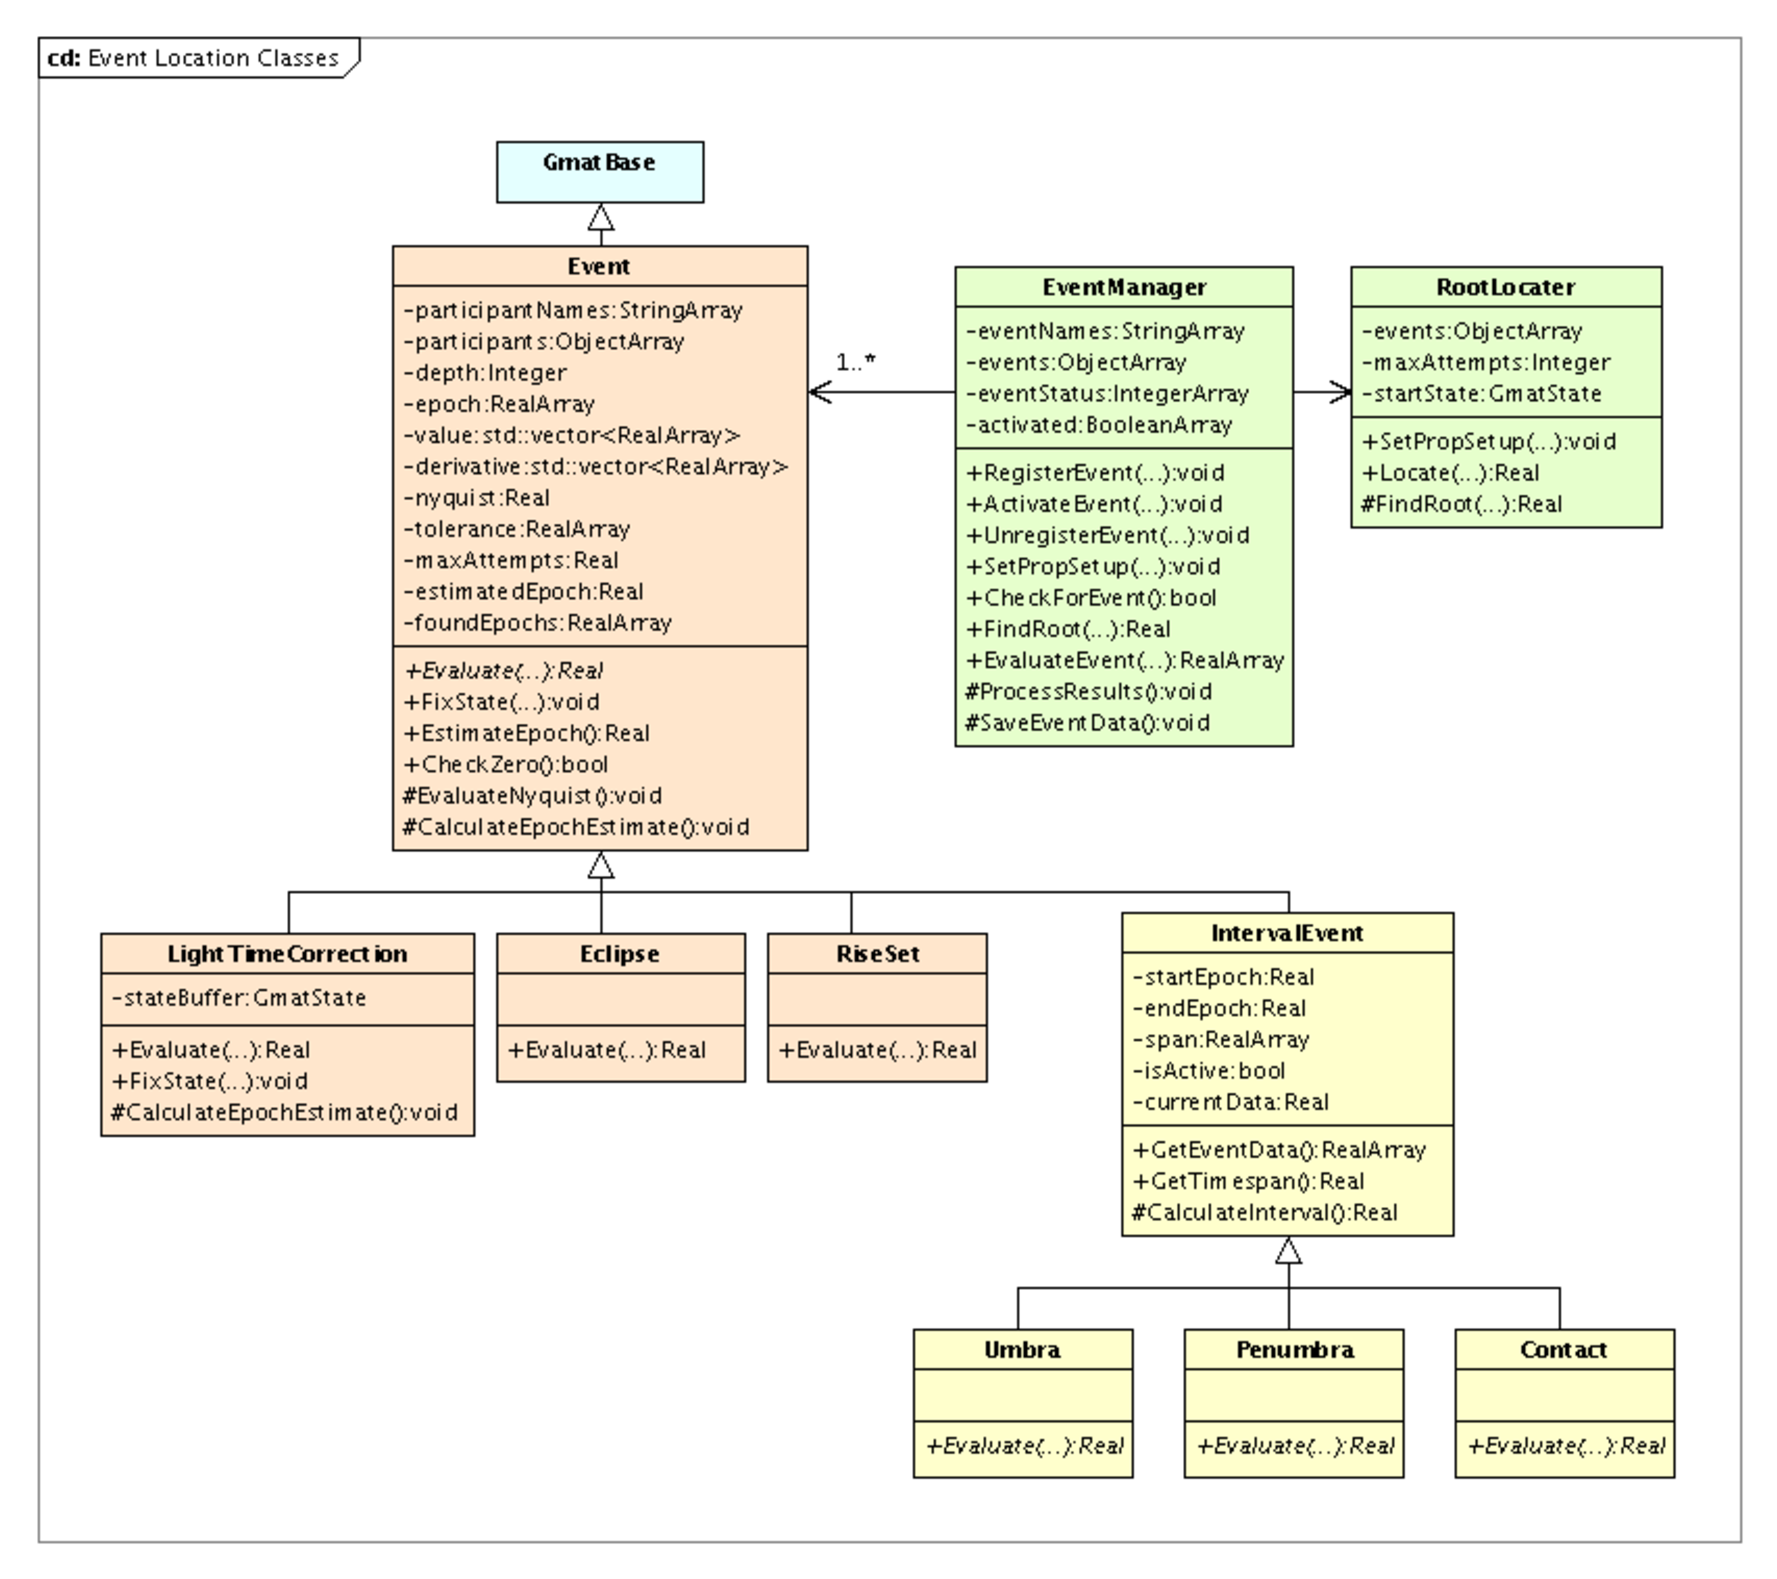
\includegraphics[scale=0.55]{Images/EventLocationClasses.eps}
% EventLocationClasses.png: 837x742 pixel, 72dpi, 29.53x26.18 cm, bb=0 0 837 742
\caption{\label{fig:EventLocationClasses}Event Location Classes}
\end{center}
\end{figure}

Figure~\ref{fig:EventLocationClasses} shows the class relationships between events, the event
manager, and the root finder.  the following paragraphs describe each of these classes in some
detail.

\subsection{Event Classes}

Three specific events are shown in the Figure~\ref{fig:EventLocationClasses}: the RiseSet event, the Eclipse event, and the LightTimeCorrection event.  In addition, the IntervalEvent class and three specific interval events are shown.  In general, event classes are implemented by deriving a class from the Event or IntervalEvent base class, implementing the Evaluate() method to supply event function and derivative data, and if needed, implementing the FixState() method to preserve state data at a specific epoch.  IntervalEvent classes implement additional code used to track the span of the event as well, as is described below.

\subsubsection{The Event Base Class}

All events -- discrete or interval -- are derived from the Event base class.  The Event class provides the interfaces used by the EventManager and RootFinder during the event evaluation process.

\paragraph{Event Attributes}  Each GMAT Event manages its list of objects participating in the event calculation, a ring buffer of the event function values and derivatives, and data identifying the critical frequency (i.e. the Nyquist frequency) specific to the event.  These data are stored in the following data members of the Event class.

\begin{itemize}
\item \textbf{StringArray participantNames}:  Names of the objects that are needed to calculate the event function and derivative information.  These names correspond to objects in the currently running model.
\item \textbf{ObjectArray participants}:  Pointers to the objects that participate in the Event's calculations.
\item \textbf{Integer depth}:  The depth of the ring buffer that tracks the event function values and derivatives.
\item \textbf{RealArray epoch}:  Epoch data for the ring buffer.
\item \textbf{std::vector<RealArray> value}:  Event function vectors for the ring buffer.
\item \textbf{std::vector<RealArray> derivative}:  Event function derivatives for the ring buffer.
\item \textbf{Real nyquist}:  The critical frequency for the event.  This parameter is set to the largest Nyquist frequency in the event; propagation should be performed with step sizes of 1.0/nyquist or smaller in order to catch all of the events in a propagation span.
\item \textbf{Real tolerance}: Numerical tolerance needed for convergence; the event function should evaluate to a magnitude less than this value for located events.
\item \textbf{Real maxAttempts}:  The maximum number of root finding attempts allowed for this event.
\item \textbf{Real estimatedEpoch}:  The estimated epoch for an event, estimaed using the current ring buffer data through a call to EstimateEpoch().
\item \textbf{RealArray foundEpochs}:  The array of event location epochs that have been found.
\end{itemize}

\paragraph{Event Methods}  The Event class inherits code functionality from GmatBase, and
overrides methods as needed to provide Event specific functionality.  The Initialize() method, in particular, is overridden but not listed here since all GmatBase subclasses implement that method when needed.

\begin{itemize}
\item \textbf{Real Evaluate(Integer status) = 0}:  Derived classes implement this method to evaluate the event function and derivative function, filling the resulting data into the epoch, value, and derivative data structures.
\item \textbf{void FixState(GmatBase* obj, bool LockState)}:  Mechanism used to preserve the state data for a specified object -- usually a participant in the event -- for later use in event evaluation.  This method is called when event evaluation requires data at different epochs, so that the data for one object can be preserved prior to propagation, and then accessed at a post-propagation epoch.
\item \textbf{Real EstimateEpoch()}:Provides an estimated a.1 ModJulian epoch for the event.  The estimated epoch is calculated in the CalculateEpochEstimate() method.
\item \textbf{bool CheckZero()}:  Tests to see of the current event function evaluates to an event location, within the specified tolerance.
\item \textbf{void EvaluateNyquist()}:  Method called during initialization to determine the Nyquist frequency for the event.  The Event::Initialize() method calls this protected method.  Derived classes should override this method with their own version of the method if the default Nyquist frequency, 1.0e-99 Hz -- producing basically an unbounded maximum propagation step size -- is not correct.
\item \textbf{void CalculateEpochEstimate()}:  Estimates the epoch of the event based on the event's internal data.  The default implementation uses the data in the ring buffers to interpolate the event epoch.  This method requires that the ring buffer data brackets one or more zero crossings or extrema; events that do not bracket must override this method.
%\item \textbf{}:
\end{itemize}

\subsubsection{Sample Event Subclass: The LightTimeCorrection Class}

The classes derived from the Event class all follow a similar implementation pattern; rather than repeat that pattern in this text, a representative example of a discrete event is presented here.  The LightTimeCorrection class is the most complex of these classes in the figure, so it was selected for this example.

Light-time correction is a calculation that accounts for the finite light propagation time between two participants when calculating a physical quantity.  It is used, for example, when calculating a range measurement to account for the motion of the participants as the ranging signal travels from one to the other.  Since the LightTimeCorrection event needs to preserve state data at one epoch while the RootFinder propagates to a different epoch, it uses both the FixState() method and the Evaluate() method.  The event function for light time correction is the range difference between the light-time calculated distance (that is, the speed of light times the time interval that the signal is in transit), and the range calculated from the state vectors of the participants, where the participant acting as the receiver has its location evaluated at the time the signal is received, and the transmitter's location, at the time the signal left the transmitting participant.

\paragraph{LightTimeCorrection Attributes}

\begin{itemize}
\item \textbf{GmatState stateBuffer}:  The buffer used to temporarily store state data for one participant in the calculation.  For corrections that are tagged with the reception time, the buffer is used to save the state of the receiving participant while the RootFinder propagates backwards to the transmission epoch.
\end{itemize}

\paragraph{LightTimeCorrection Methods}

\begin{itemize}
\item \textbf{Real Evaluate(Integer status)}:  Calculates the event function and its derivatives, as defined in GMAT's mathematical specifications\cite{mathSpec}.
\item \textbf{void FixState(GmatBase* obj, bool lockState)}:  Tells the event to buffer the state of the input object.  lockState is not used in the light time correction, but is supplied to make the method conform to the base class method that is overridden here.
\item \textbf{void CalculateEpochEstimate()}:  Estimates the epoch of a light time endpoint using the range calculated from the participant locations.  This method uses the stateBuffer data as the state of one of the participants for one of the end points, and the current (possibly propagated) state of the other participant as the second endpoint in the calculation.
\end{itemize}

\subsubsection{The IntervalEvent Base Class}

To be written.

\paragraph{IntervalEvent Attributes}

\paragraph{IntervalEvent Methods}

\subsection{The EventManager Class}

Event function monitoring and event location are controlled through the EventManager class.  Each Sandbox contains an EventManager.  The pointer to the local EventManager is passed to each command as the Mission Control Sequence is initialized in the Sandbox.  Commands use this event manager to register, access, evaluate, and locate events as the sequence executes.  The EventManager acts as a mediator between all of the objects in the location process: it tracks the Events and their status, passes PropSetup objects and control to the RootFinder when an event is ready to be located, and passes event function data to any object that needs it.

The sequence diagrams (Figures~\ref{fig:EventLocationSD} and~\ref{fig:MeasurementLocationSD}) show how the EventManager functions in these roles.  The class attributes and methods are described here:

\paragraph{EventManager Attributes}  The core attributes of the EventManger are the data structures that track the Event objects and their status, along with the RootLocator used to find the precise event location.

\begin{itemize}
\item \textbf{StringArray eventNames}:  String descriptions of the events that are registered with the event manager.
\item \textbf{ObjectArray events}:  The current set of Event objects registered with the EventManager.
\item \textbf{RootLocater locater}:  The root locator that searches for event locations once an event has been detected.
\item \textbf{IntegerArray eventStatus}:  The current status of the event.  This event status flag can be set to SEEKING, ZERO\_BRACKETED, EXTREMA\_BRACKETED or LOCATED for each active event.  These values are enumerated in the EventStatus enumeration, a member structure in the EventManager.
\item \textbf{BooleanArray activated}:  Array of flags indicating if the corresponding Event should be checked.  Deactiviated Events are skipped in the evaluation process.
\end{itemize}


\paragraph{EventManager Methods}

\begin{itemize}
\item \textbf{void RegisterEvent(Event newEvent)}:  Adds an event to the EventManager.  When an event is added, it is also evaluated, setting the initial function values on the Event.  Added events are automatically active until deactivated by a call to ActivateEvent().
\item \textbf{void ActivateEvent(Event theEvent, bool makeActive)}:  Sets the activated state for an event.  This call turns on or off event calculations for the specified event, based on the setting of the makeActive flag.  When an inactive event is made active, its ring buffer is cleared and the Evaluate() method is called, providing the initial event function data.  The method is idempotent: activating an active event has no affect, nor does deactivating a deactiveated event.
\item \textbf{void UnregisterEvent(Event theEvent)}:  Removes an event from the event queue.
\item \textbf{void SetPropSetup(Estimator::PropSetup* ps)}:  Sets the PropSetup that will be used for event location.
\item \textbf{bool CheckForEvent()}:  Tests to see if and event has occurred or if an extremum has been encountered.
\item \textbf{Real FindRoot(Integer whichOne)}:  Tells the EventManager to call the RootFinder to locate the specified event.
\item \textbf{RealArray EvaluateEvent(Integer whichOne)}:  Returns the current event function values for the specified event.  This method can be used to retrieve event function data for use in parameters and data subscribers.
\item \textbf{void ProcessResults()}:  Performs processing to determine the event state.
\item \textbf{void SaveEventData()}:  Saves event data so it can be accessed later.
\end{itemize}

\subsection{The RootFinder Class}

Event location in GMAT requires a search over time for a zero of one or more event function values.  The obtained value must fall within a set tolerance of zero; this tolerance is set on each Event object, and defaults to 1.0e-7.  It can be overridden in the Event code.  The RootFinder class performs the search for the function roots.  It works with methods on the Event classes to
retrieve an estimate of the epoch of the root, then drives a PropSetup to move the participants that need propagation to the target epoch.  Finally, it calls the Event's Evaluate() method to determine the current values of the event function, followed by a check for convergence.

The key RootFinder members are described here:

\paragraph{RootFinder Attributes}  The RootFinder uses several internal data structures to manage the root finding process.  These data structures, described here, are transitory; they are only current during the root finding process, and may be stale if examined outside of that process.

\begin{itemize}
\item \textbf{ObjectArray *events}:  The current set of Events that are used to search for roots.
\item \textbf{Integer maxAttempts}:  Maximum number of attempts allowed to find the root.  When maxAttempts is exceeded, the RootFinder posts a message, discards the event location data, and returns.  If a root is located, Events that are being examined because an extremum was detected store the root data, reset the counter, and then search for an additional root.
\item \textbf{GmatState startState}:  The state of all participants at the start of the root search.  This state is restored to the participants at the end of the root finding process.
\end{itemize}

\paragraph{RootFinder Methods}  The root finder uses a propagator set by the EventManager, along with a list of events that may contain roots.  The following methods are used in teh root location process:

\begin{itemize}
\item \textbf{void SetPropSetup(Estimator::PropSetup* ps)}:  Passes a propagator to the root finder.
\item \textbf{Real Locate(ObjectArray \&whichOnes)}:  Public method called by the EventManager to locate all triggered events.  The input ObjectArray contains pointers to all of the Events that need evaluated.  The RootFinder evaluates these events in the order that they are entered into the array.
\item \textbf{Real FindRoot(Event *whichOne)}:  This method is the core root finding code.  It manages all of the propagation and event evaluation needed to find the roots of the event functions.
\end{itemize}


\chapter{Measurement Classes and Measurement Models}

\chapauthor{Stephen P. Hughes}{NASA/Goddard Space Flight Center}
\chapauthor{Darrel J. Conway}{Thinking Systems, Inc.}
\chapauthor{Matthew P. Wilkins}{Schafer Corporation}

The Measurement classes define the interfaces used to work with measurement data during the estimation process.  These classes provide access to the observation data, typically provided by way of a data file, using a helper object derived from the MeasurementReader base class.  The Measurement classes provide methods that calculate the expected value of a specific measurement type, along with the derivative data needed for estimation.  These data include calculation of expected measurements, measurement partials, determination of measurement feasibility, and interactions with root finders to determine tracking schedules and light time corrections.  A measurement object acts as a participant in the measurement, as the measurement object contains estimated states associated with measurement errors.

The measurement hierarchy consists of a base class and a tiered hierarchy of derived classes as shown in Figure~\ref{fig:MeasurementClasses}.  The following sections discuss each class in the hierarchy in detail, starting with the Measurement base class.

\begin{figure}[htbp]
\begin{center}
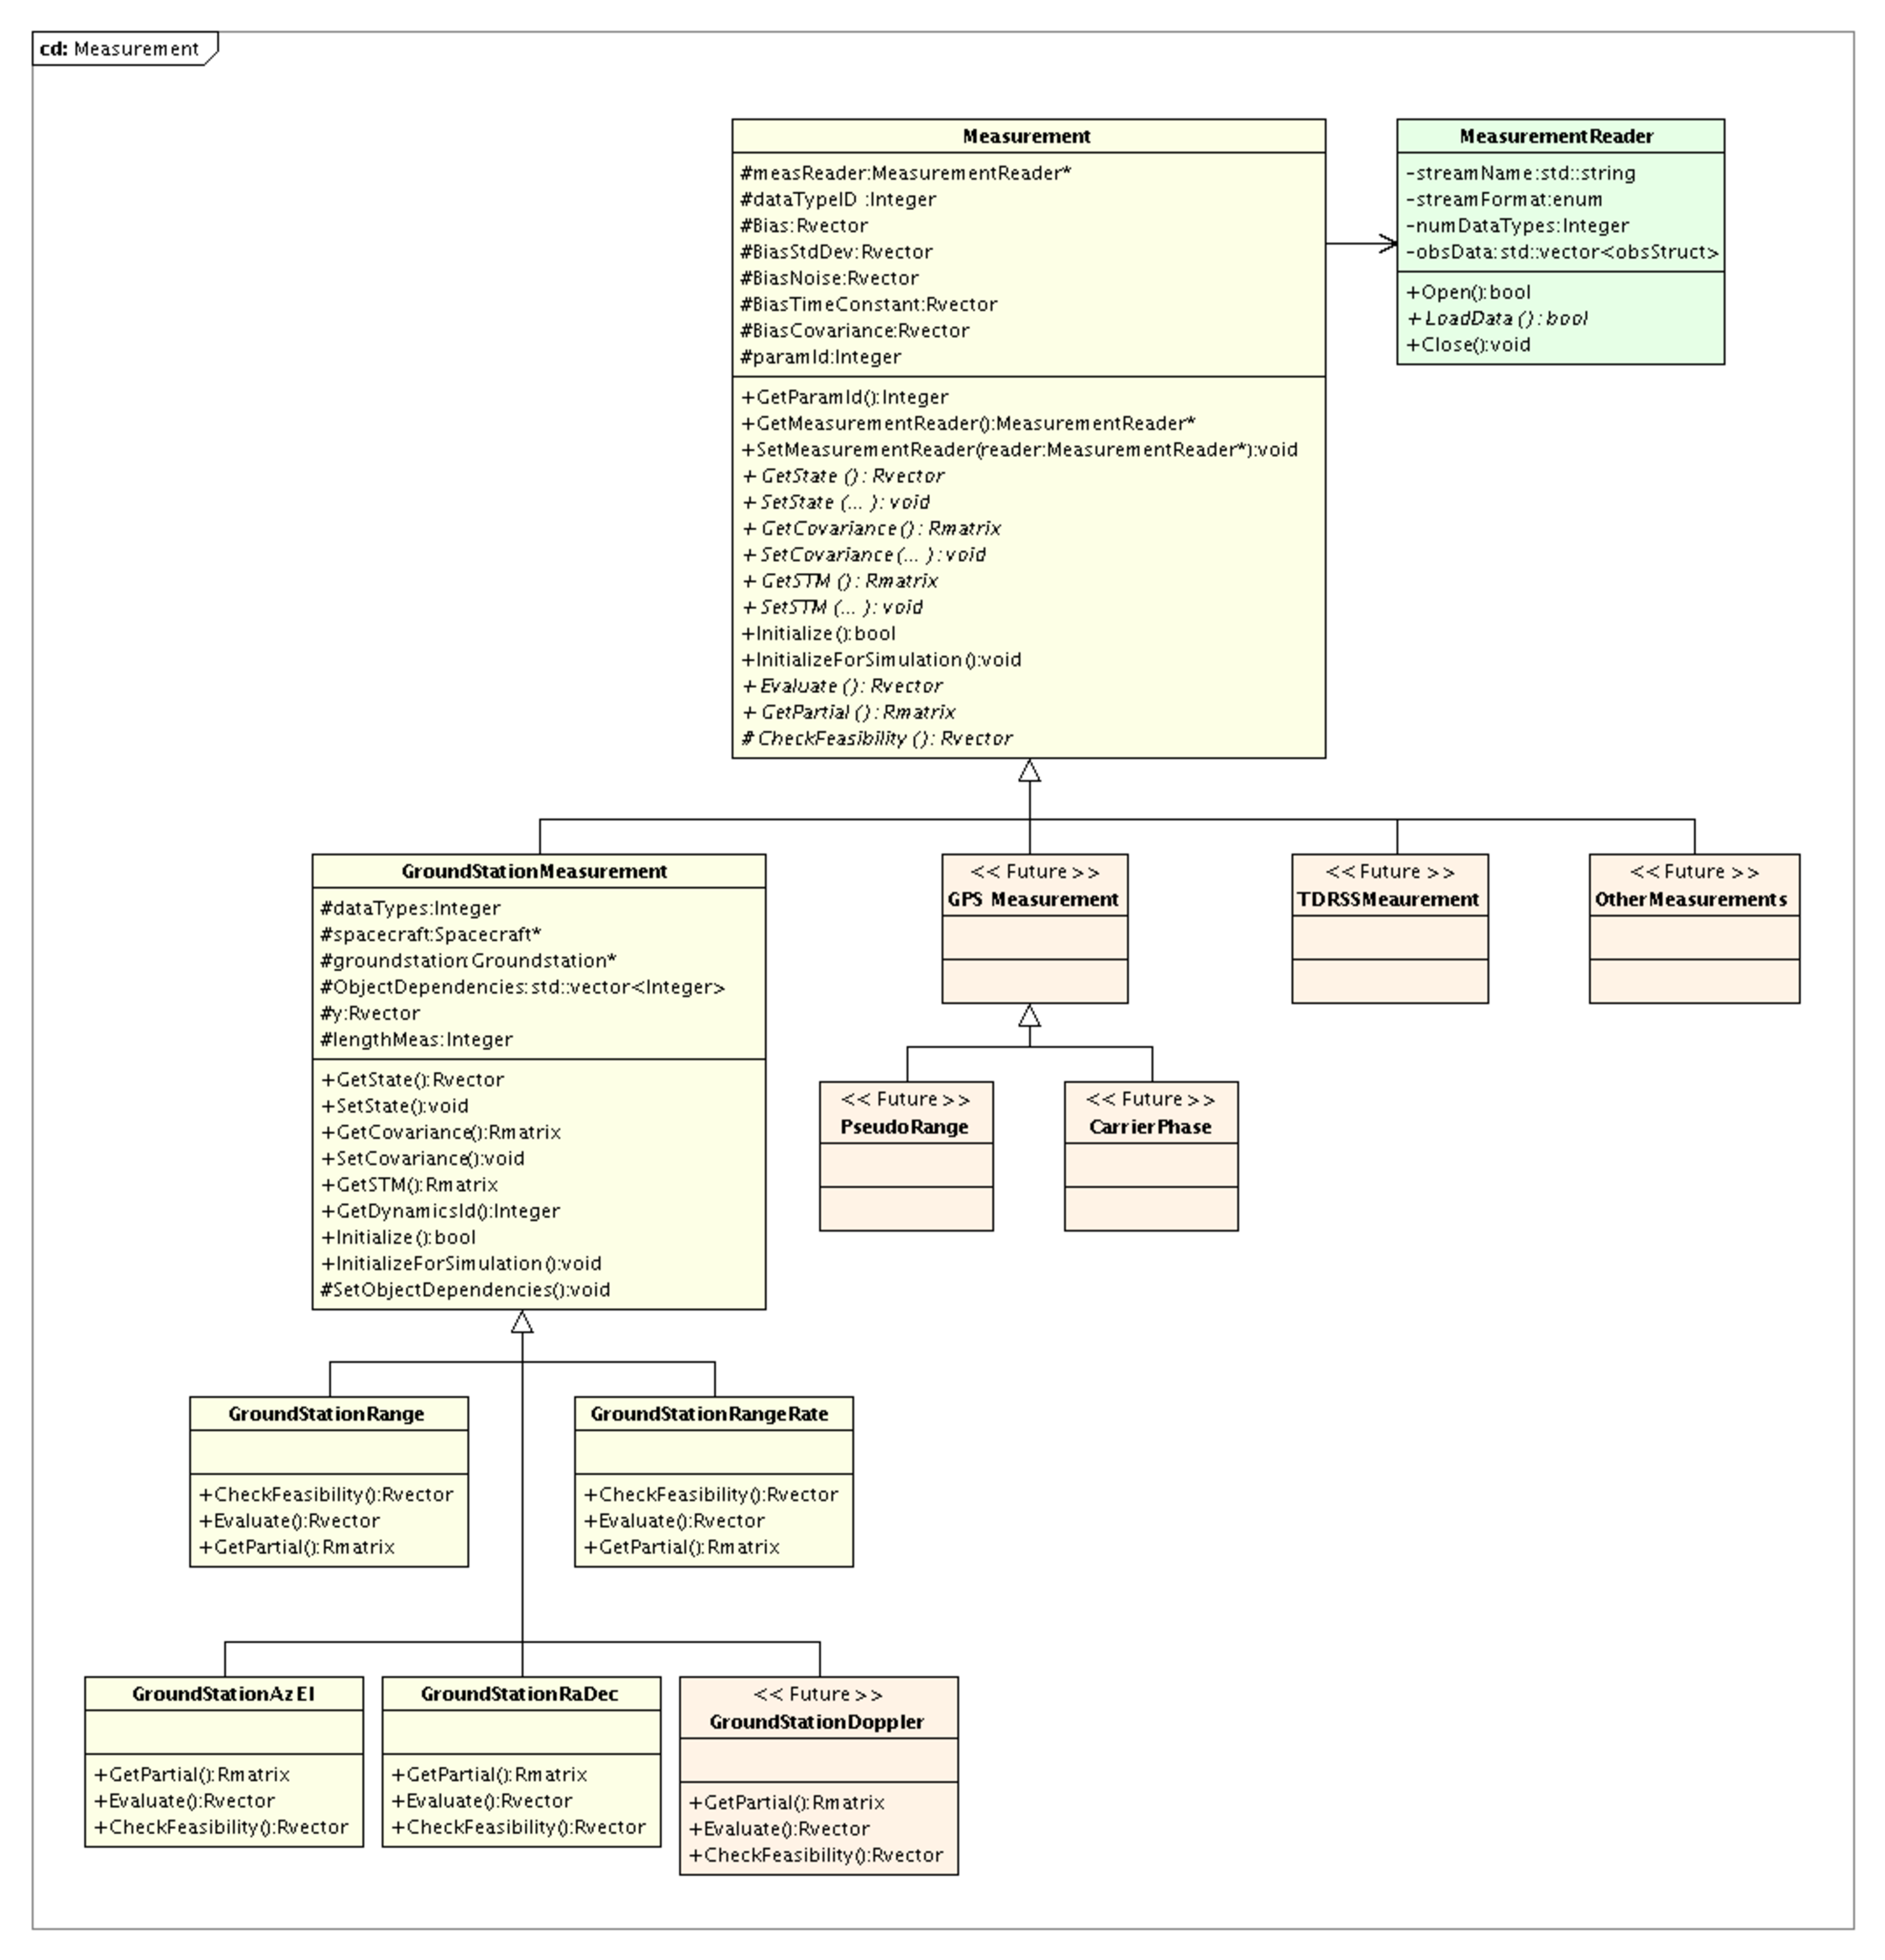
\includegraphics[scale=0.43]{Images/MeasurementClasses.eps}
% MeasurementClasses.png: 1061x1104 pixel, 72dpi, 37.43x38.95 cm, bb=0 0 1061 1104
\caption{\label{fig:MeasurementClasses}The Measurement Class Hierarchy}
\end{center}
\end{figure}

\section{The Measurement Class}

The Measurement base class contains member data and functions associated with all measurement objects as well as data associated with parameters that are set by the user when configuring the measurement object.  Examples of these data include the measurement file name and format, the data types to be processed from the file, and measurement stochastic properties such as biases and time constants.

The Measurement class defines many of the interfaces implemented in the derived classes so that the estimation process can work with measurement objects using base class references and pointers.  These interfaces are defined as either overridable or abstract (that is, pure virtual) methods on the Measurement base class.  The derived classes implement custom versions of these methods that are specific to the measurement type being implemented.  The data members of the Measurement base class are described below, followed by descriptions of the methods provided in the Measurement base class.  Finally, we will describe the MeasurementReader helper class before moving to the definitions of the derived classes.

\subsection{Measurement Members}

\paragraph{Member Attributes}

The list below describes the data elements provided in the Measurement base class to support the derived classes.  These elements are designed to facilitate access to measurement information through calls to a Measurement instance pointer.  Some Measurement objects provide multiple data elements.  For that reason, some of the data members listed here gain a dimension over what might be expected for single-valued measurements.  For example, the ground station RA/Dec measurement type returns two values for each measurement: the right ascension and declination values, so the methods that calculate these values return an Rvector rather than a Real number.  Since there are
Measurement classes that have this multivalued return requirement, GMAT uses an Rvector for the data, even when the return value is a single number.

The data members of the Measurement are:

\begin{itemize}
\item \textbf{MeasurementReader *measReader}:  The MeasurementReader that supplies the observation data. This pointer can be NULL when simulating data.
\item \textbf{Integer dataTypeID}:   An integer containing the Id for the data type.  Although the user may specify several data types on a measurement object, GMAT creates an object for each data type during initialization.  Each object has an Id associated with its data type which is specified by dataTypeId.
\item \textbf{Rvector Bias}:  A vector of real numbers containing the measurement biases.  These data can be estimation state parameters.
\item \textbf{Rvector BiasStdDev}:  A vector of real numbers containing the standard deviations of the biases. These data can be estimation state parameters.
\item \textbf{Rvector BiasNoise}:  A vector of real numbers containing the noise in the measurement biases. These data can be estimation state parameters.
\item \textbf{Rvector BiasTimeConstant}:  A vector of real numbers containing the time constants for the measurement biases. These data can be estimation state parameters.
\item \textbf{Rvector BiasCovariance}:  A vector of real numbers containing the bias covariances.
\item \textbf{Integer ParamId}:  ID for the type of measurement parameter?
\item \textbf{Integer numDataTypes}:  The number of data types the user specified on the measurement object. During measurement initialization, a new object is created for each data type specified on the measurement object.
\end{itemize}

\paragraph{Class Methods}

The Measurement class includes the following methods designed to make access to measurement data as generic as possible by the classes that use Measurement objects.  Many of these methods are abstract (pure virtual in C++ terminology): they are defined in this base class, but no implementation is provided in the base class.  The abstract classes can be identified by an ``= 0'' suffix in this list.

\begin{itemize}
\item \textbf{enum MeasurementFormat}: An enumeration defining the supported measurement formats.  Note: This enumeration is not a class member; it is a member of the Gmat namespace.
\item \textbf{Integer GetParameterId()}: A method to determine the integer id for solve-for and consider parameters on the measurement object.  This is how the system converts from the string definition provide by the user, say MauiGSRange.Bias,to a numeric Id.  <DJC: Not sure of this part.>
\item \textbf{MeasurementReader *GetMeasurementReader()}:  Retrieves a pointer to the
MeasurementReader.
\item \textbf{void SetMeasurementReader(MeasurementReader *reader)}:  Sets the pointer to the MeasurementReader.
\item \textbf{virtual Rvector\& GetState() = 0}: Retrieves the state vector.
\item \textbf{virtual void SetState(Rvector\& newState) = 0}:  Sets the state vector to match the provided data.
\item \textbf{virtual Rmatrix\& GetCovariance()= 0}:  Retrieves the covariance matrix.
\item \textbf{virtual void SetCovariance(Rmatrix\& newCovariance) = 0}:  Sets the covariance matrix data.
\item \textbf{virtual Rmatrix\& GetSTM() = 0}: Retrieves the state transition matrix.
\item \textbf{virtual void SetSTM(Rmatrix\& newSTM) = 0}: Sets the STM matrix data.
\item \textbf{virtual bool Initialize()}: Prepares the Measurement object for use in a Sandbox.
\item \textbf{virtual void InitializeForSimulation()}:  Prepares the Measurement object for use during measurement simulation.
\item \textbf{virtual Rvector\& Evaluate() = 0}:  Calculates the expected observation value.
\item \textbf{virtual Rmatrix\& GetPartial() = 0}:  Retrieves the measurement partial derivative matrix.
\item \textbf{virtual Rvector\& CheckFeasibility() = 0}:  Checks to see if a measurement can be made using the current state information.
\end{itemize}

\section{GroundstationMeasurement}

Measurements that are made at a ground station are modeled using the GroundStationMeasurement class.  Data and member functions that are common to all Ground Station measurements are located on the GroundStationMeasurement class, including the participants in the measurement process, Get/Set functions, and common modeling algorithms.   Below we discuss in detail all member data and functions.

\subsection{GroundstationMeasurement Members}

\paragraph{GroundStationMeasurent Attributes}

\begin{itemize}
\item \textbf{Integer dataTypes}:  ???
\item \textbf{Spacecraft *spacecraft}:  A pointer to the spacecraft that is participating in the measurement. This pointer is set during measurement initialization.
\item \textbf{Groundstation *groundstation}:  A pointer to the ground station that is participating in the measurement.  This pointer is set during measurement initialization.
\item \textbf{std::vector<Integer> ObjectDependencies}: A vector of integers that contains information on how participants on a measurement object map to participants in the overall estimation problem.  In general, the participants on a measurement are a subset of the participants for the estimation problem.  The ObjectDependencies is used primarily to determine partial derivatives and ensure they are placed in the correct location in the overall partial derivative array.  The ESM maintains an array of pointers, called ObjectsVector, to the participant associated with each state chunk in the estimation problem.  The ObjectDependencies array is the same length as ObjectsVector.  If, for example, element 1 of ObjectDependencies is zero, then the first object in the estimator's participant list is not a participant in the measurement.  If element 1 is nonzero, then the integer is associated with the participant Id used internally by the measurement.  The ObjectDependencies array is set during initialization when the Measurement Manager makes a call to initialize the measurement.
\item \textbf{Rvector y}:  The vector of calculated measurements.
\item \textbf{Integer lengthMeas}:  ???
\end{itemize}

\paragraph{}GroundStationMeasurement Methods:

\begin{itemize}
\item \textbf{SetState}:  Given a state value and id, this method updates the state on the measurement object.
\item \textbf{GetState}:  Given a state id, this method gets the state from the measurement object.
\item SetCovariance:  Given a covariance matrix and the state id, this method updates the state's covariance on the measurement object.
\item \textbf{GetCovariance}:  Given a state id, this method gets the state's covariance from the measurement object.
\item \textbf{GetSTM}: Given a state id, this method gets the states' STM.
\item \textbf{GetDynamicsId}:  Given a state Id, this method returns the ODE model ID for use in propagation of the state and it's STM.  Not implemented yet for measurement.
\item \textbf{Initialize}:  This method makes a call to the file reader and gets the observations and epochs from the requested data type.  If there are multiple data types on the measurement, the measurement object concatenates them into the Obs and Epochs Arrays.  These are then extracted by the measurement manager later in the initialization process.     For each data type, a new object is created and pointers to the object's participants are set.  (Matlab currently only supports one data type per measurement.  Not a difficult mod though)
\item \textbf{InitializeforSimulation}:  This method prepares a measurement object for simulation.  The process is similar to the Initialize method on GroundStationMeasurement, with the exception the reading and managing observations and epochs is not required.
\item \textbf{GetDataTypeId}:  This method returns the integer Id for the measurement type, given the string name for the measurement.
\item \textbf{SetObjectDependencies}:  This method takes as input an array of pointers to the participants in the estimation state vector.   The method steps through each element in the input array and determines if it points to any of the measurement participants.   If not, then the element in ObjectDependencies is set to zero.  If so, then the element is set to the Id of the participant used internally by the measurement object.
\end{itemize}

\section{GroundStationRange}

The GroundStationRange class is derived from the GroundStationMeasurement class, and performs modelling range measurements, measurement feasibility, and partial derivatives, and light time iteration.

\subsection{GroundstationRange Members}

\paragraph{GroundStationRange Attributes}

None.  The data members in the GroundStationMeasurement class are sufficient for this class.

\paragraph{GroundStationRange Methods}

\begin{itemize}
\item \textbf{CheckFeasibility}:  This method evaluates the feasibility function for the range measurement. If the value of the feasibility function is positive, then the conditions required to perform a measurement are met.  If the feasibility function is negative, conditions are not met.  Event locators determine the roots of the feasibility function to determine tracking data scheduling.
\item \textbf{Evaluate}:  The evaluate function calculate the computed value of the measurement based on the current state of the participants.
\item \textbf{GetPartial}:  This method returns the requested partial derivative based given a participant Id and the state Id.  The participant Ids are contained in the array ObjectDependencies.  This method is called by the measurement manager to determine individual partials. The measurement manager assembles the entire partial derivative from the pieces returned by the measurement object.
\end{itemize}

\section{The MeasurementManager Class}

The measurement manager functions as the interface between the Estimator and the measurement objects
defined by the user.  The primary jobs of the measurement manager are

\begin{itemize}
\item To coordinate measurement data and provide observed and computed values to the estimator
\item To maintain the sorted list of observed measurement quantities from all measurement sources.
\item To assemble the H matrix for each measurement based on state information and the partials map
provided by the measurements.
\end{itemize}


\chapter{\label{ch:MeasurementCorrections}Measurement Corrections}

\chapauthor{Darrel J. Conway}{Thinking Systems, Inc.}

To be written.

\section{Introduction}

\section{Additive Corrections}

\section{Event Based Corrections}

\begin{figure}
\begin{center}
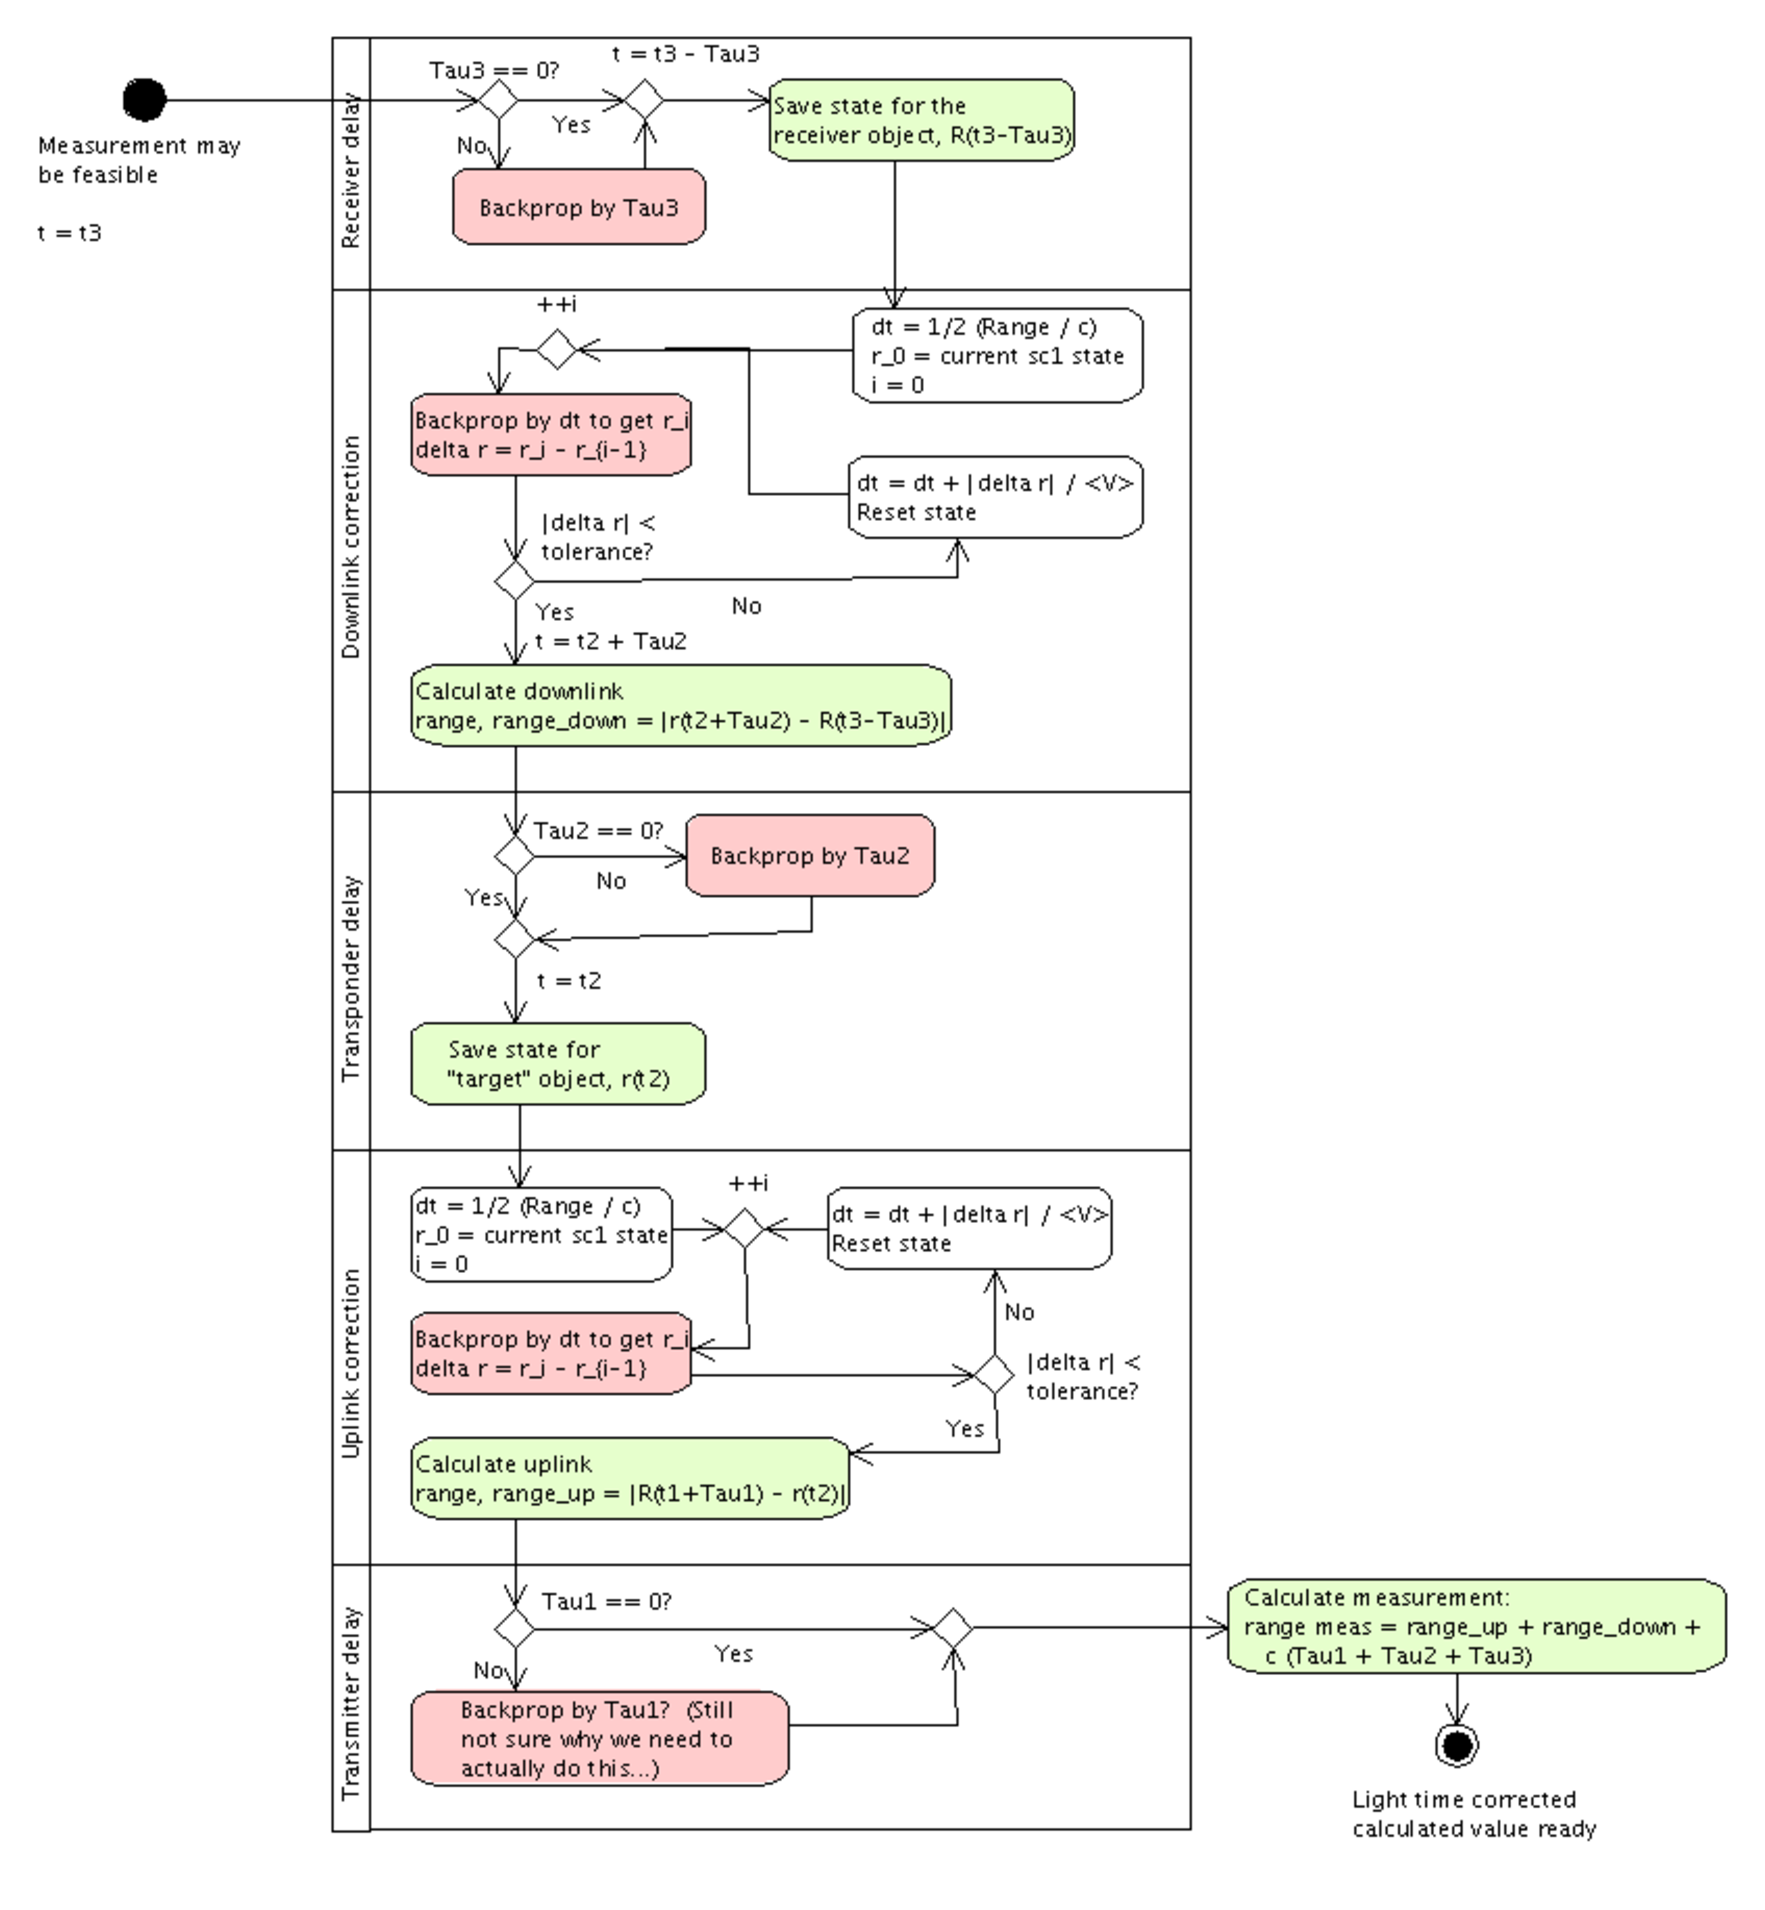
\includegraphics[scale=0.52]{Images/EventLocationLightTimeCorrection.eps}
% EventLocationLightTimeCorrection.png: 831x901 pixel, 72dpi, 29.32x31.79 cm, bb=0 0 831 901
\caption{Steps in Light Time Correction: Two Way Range}
\end{center}
\end{figure}


\begin{figure}
\begin{center}
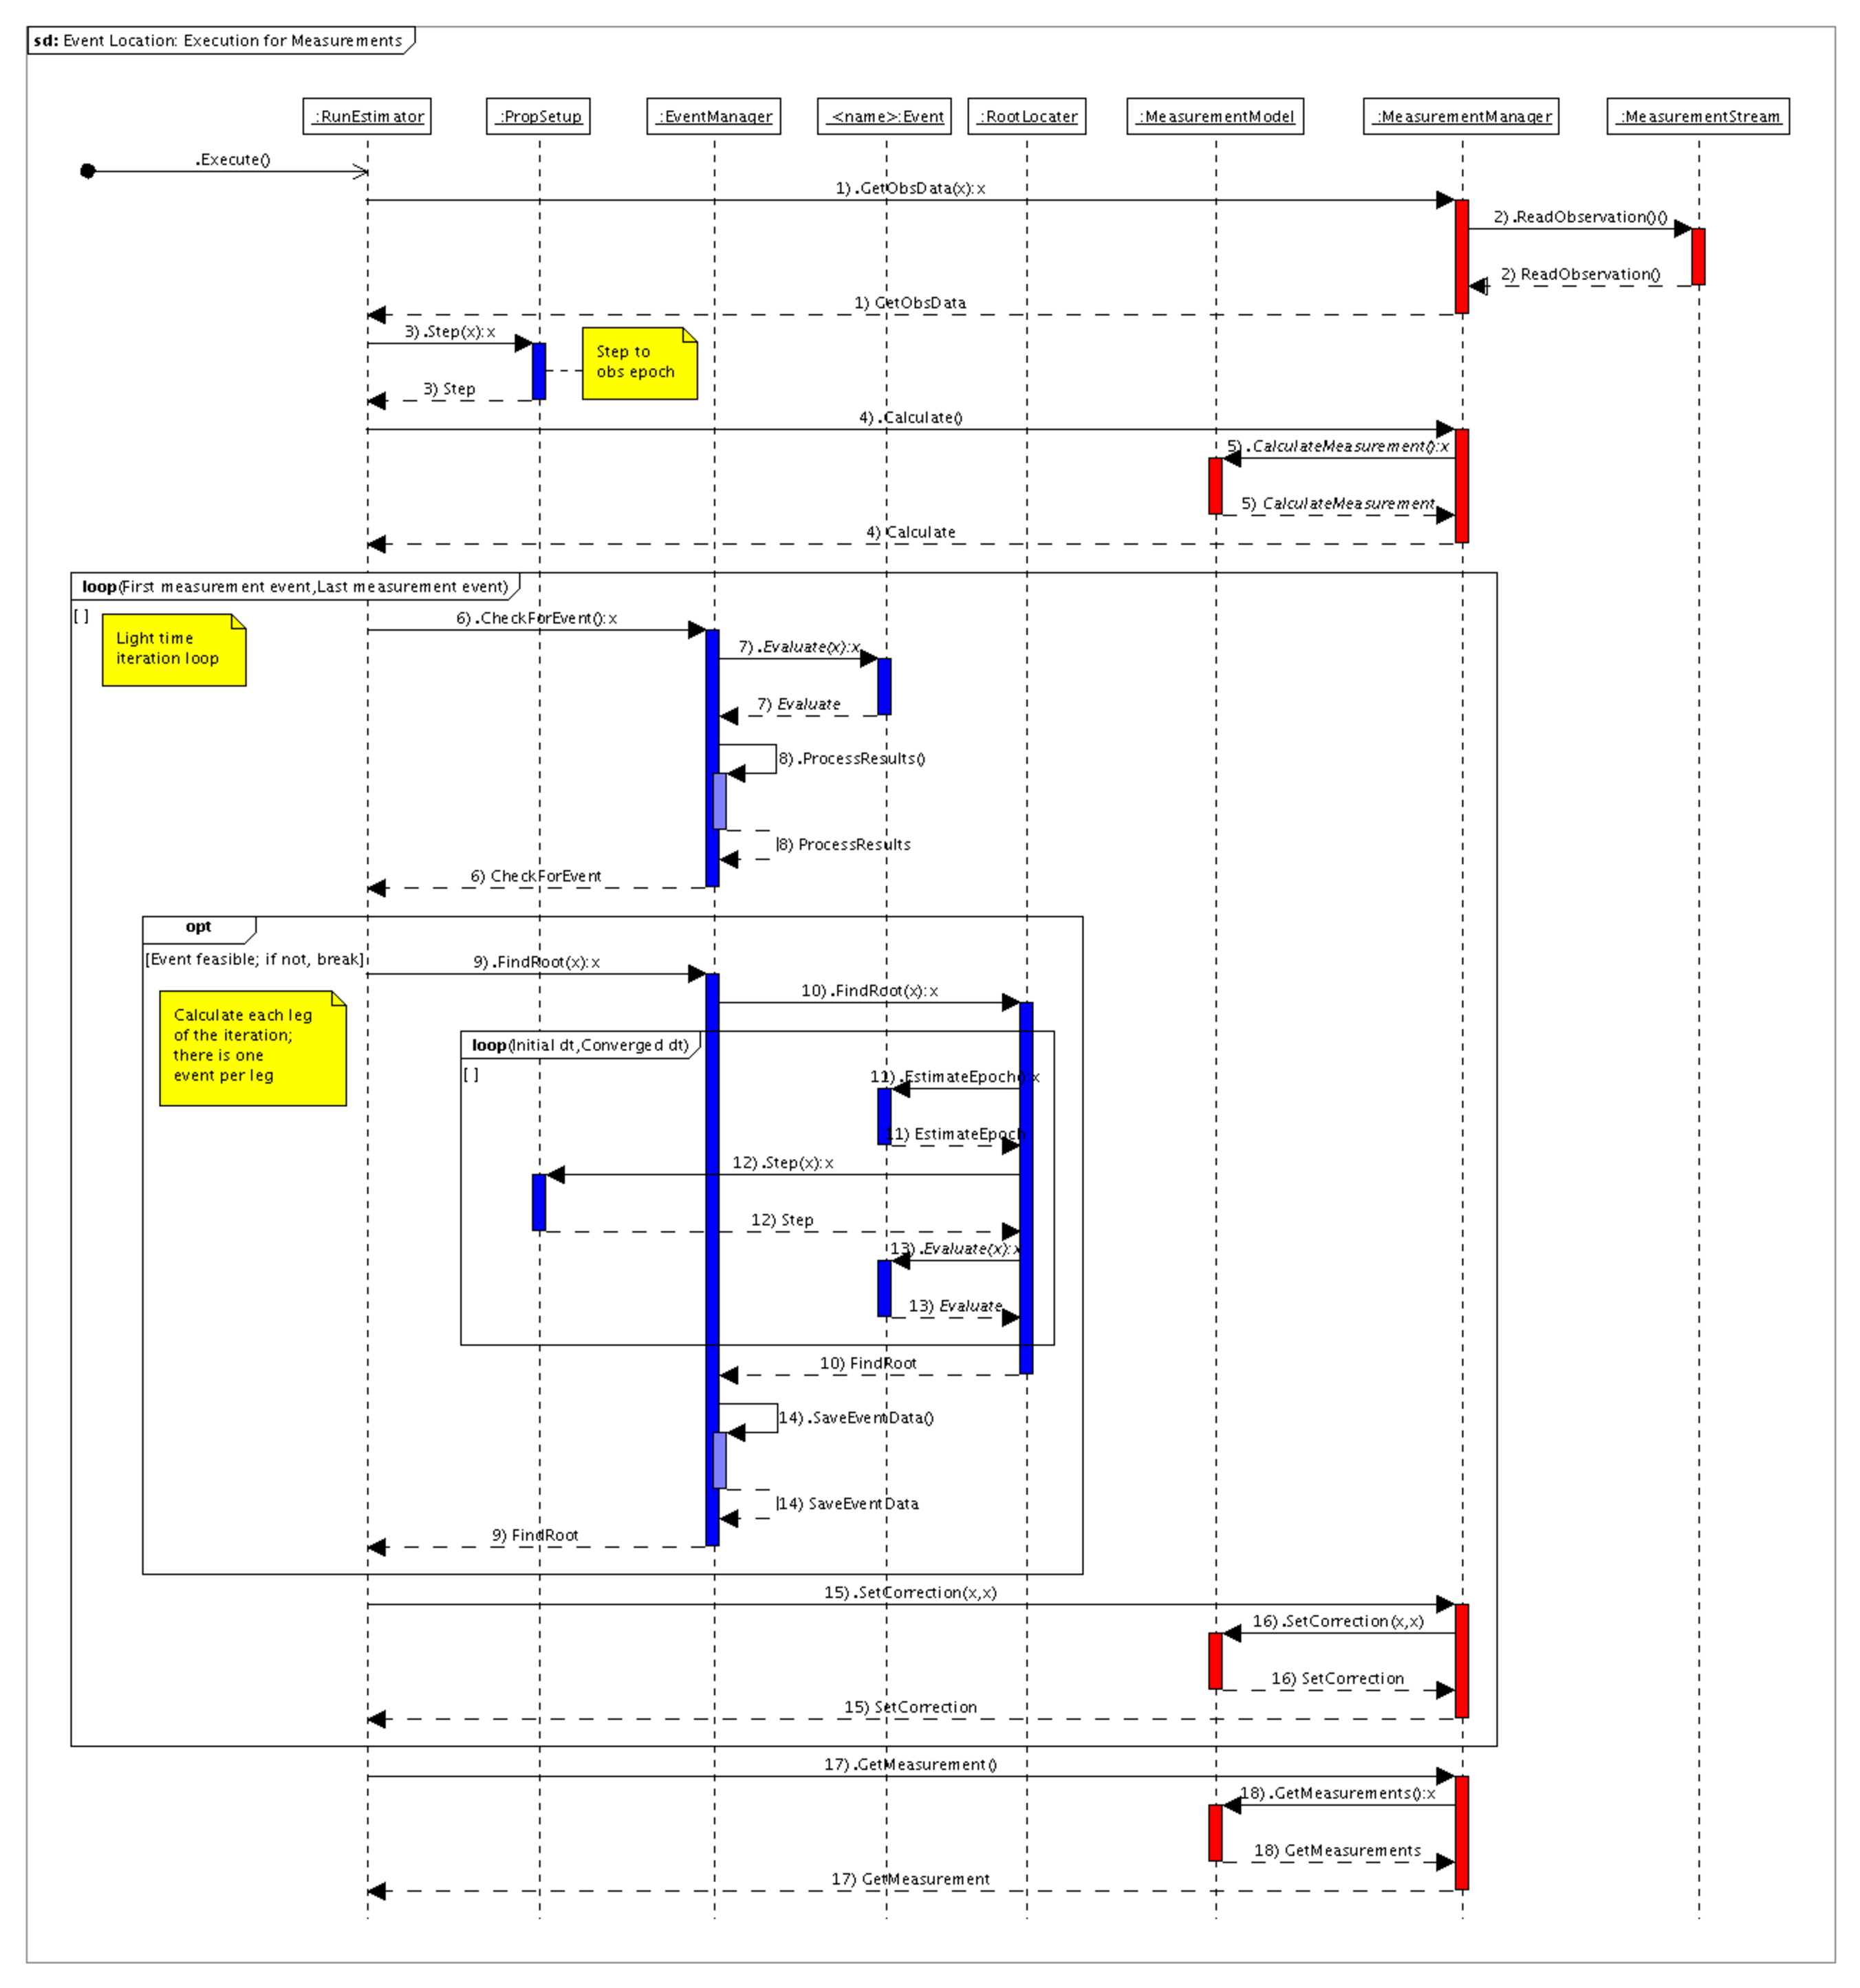
\includegraphics[scale=0.36]{Images/EventLocationExecutionforMeasurements.eps}
% EventLocationExecutionforM...ts.png: 1282x1371 pixel, 72dpi, 45.23x48.37 cm, bb=0 0 1282 1371
\caption{\label{fig:MeasurementLocationSD}Event Location for Measurements}
\end{center}
\end{figure}

\chapter{Hardware Used in Estimation}

\chapauthor{Darrel J. Conway}{Thinking Systems, Inc.}

GMAT's measurement models perform the task of calculating measurement values,
measurement derivatives, and associated properties of measurements needed for
estimation.  Many models depend on the physical characteristics of the hardware
that gathers the measurement data.  These characteristics are contained in the
hardware classes described in this chapter.

\section{Hardware Classes}

\begin{figure}[htbp]
\begin{center}
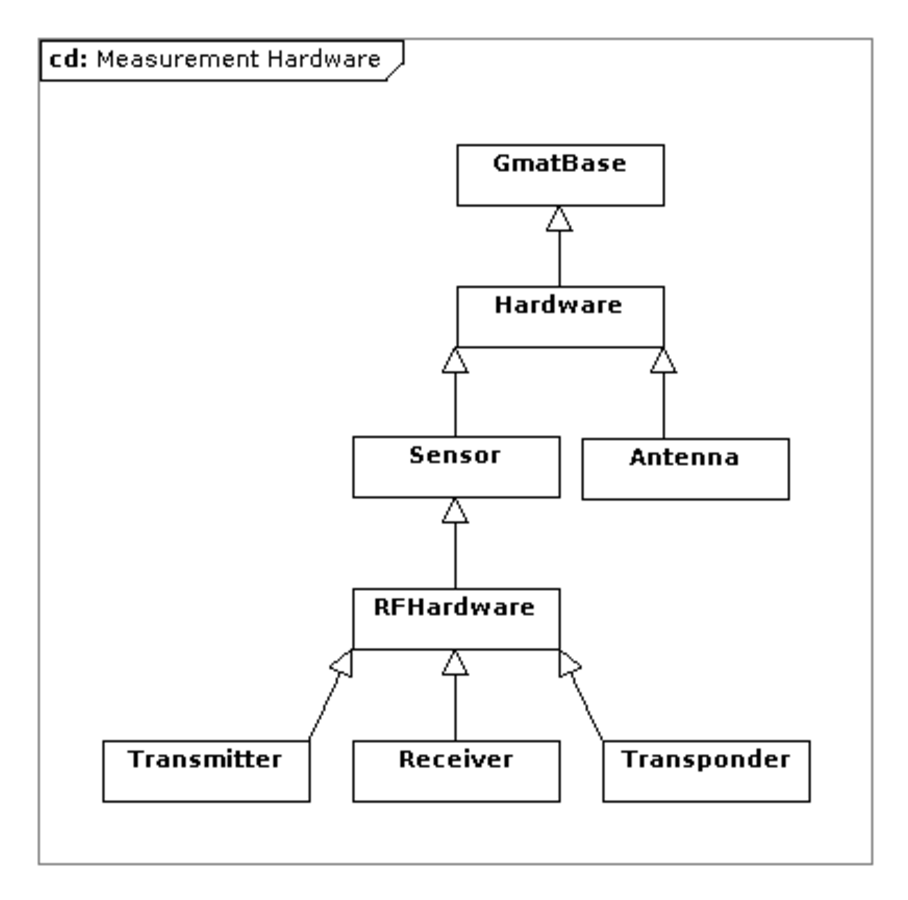
\includegraphics[scale=0.6]{Images/MeasurementHardware.eps}
% MeasurementHardware.png: 420x416 pixel, 72dpi
\caption{\label{fig:MeasurementHardware}Hardware Classes Used in Measurement
Modeling}
\end{center}
\end{figure}

\section{Estimation Interfaces}

The estimation subsystem accesses the properties and computations in the
hardware classes through a set of intefaces defined below.  The subsystem used
these interfaces to 
\begin{enumerate}
 \item \label{hw:feasibility}Evaluate signal based feasibility for a measurement
 \item \label{hw:delay}Find hardware associated delay values
 \item \label{hw:transmit}Retrieve signal properties for transmitters
 \item \label{hw:receive}Report signal properties to receivers
\end{enumerate}
\noindent
Many sensors modeled in GMAT's estimation processes have signal feasibility
constraints beyond simple line-of-sight constraints.  For example, receivers are
often constrained to specific frequency bands and optical sensors to specific
signal strengths before a measurement can be recorded.  The feasibility
interfaces (item~\ref{hw:feasibility}, above) captures these constraints. 
Detailed modeling requires that GMAT account for delays induced by electronics
in the hardware.  These delays are accessed using the interfaces supporting
item~\ref{hw:delay}.  Finally, the signal properties of transmitters need to be
accessed and passed into the signal receivers, potentially after modification
based on the signal propagation between the components.  These properties are
accessed through the transmitter and receiver interfaces,
items~\ref{hw:transmit} and~\ref{hw:receive}.

The methods supporting the estimation interfaces are defined in the Sensor
class.  The estimation hardware classes override these methods to implement the
sensor specific implementations of the methods.  GMAT's estimation subsystem
calls these interfaces to retrieve the data needed to calculate measurements and
their derivatives.  These measurement calculations are then used in the
simulation process to generate simulated measurements, or in the estimation
process to calculate the expected value of a measurement associated with teh
estimation hardware.

The following paragraphs define the interfaces that GMAT's estimation subsystem
uses for these processes.  We'll begin with a description of each method
defined fir this use in Sensor, and conclude with some representative overviews
of estimation processes that use these interfaces.



\chapter{Tracking Systems}

% \chapauthor{Stephen P. Hughes}{NASA/Goddard Space Flight Center}
\chapauthor{Darrel J. Conway}{Thinking Systems, Inc.}
% \chapauthor{Matthew P. Wilkins}{Schafer Corporation}

GMAT uses a high level construct -- the Tracking System -- to manage the
interactions between measurement models, measurement corrections, participants,
and the measurement manager.  In one sense, a tracking system is a container
for measurements.  It provides the ability to group compatible measurement
models together for use during simulation or estimation.  The tracking system
model in GMAT extends this basic container paradigm to include global
properties in a single scripted location.  GMAT's tracking system model
includes a container for measurement correction models like tropospheric
and ionospheric correction models.  These corrections are applied to all
measurements in the tracking system, as is described in this chapter.



% \part{Other Components}

\part{Estimation Examples}
\thispagestyle{empty}

%\part{Views and Interfaces}
%\thispagestyle{empty}

%\part{Utilities}
%\thispagestyle{empty}


%% $Id: GmatWorkFlow.tex,v 1.1 2008/01/31 18:04:16 dconway Exp $
\chapter{\label{chapter:WorkFlow}GMAT Work Flow}
\chapauthor{Darrel J. Conway}{Thinking Systems, Inc.}

This chapter describes, at a high level, the interactions of the objects in GMAT during a typical session.
\section{Configuring Objects}

\section{Running a Mission}

\section{Initialization}

\section{Execution}

\section{\label{section:InterfaceOverview}Interface Components}

% The interfaces to GMAT can be broken into interfaces with external system and interfaces with
% users.  The external interface component is used to provide an interface between GMAT and MATLAB.
% Other external systems may be interfaces to GMAT in future builds.  The internal interfaces are
% used to let the user control GMAT, either through custom text files called scripts, or through
% direct manipulation to objects managed in GMAT.  Figure~\ref{InterfacePackages} shows the
% main classes used to implement these interfaces.  The two major subdivisions are outlined here.
% Details of the design for these components can be found in chapters~\ref{chapter:ScriptRW},
% \ref{chapter:TheGui}, and \ref{chapter:ExternalInterfaces}.

%\begin{figure}[htb]
%\begin{center}
%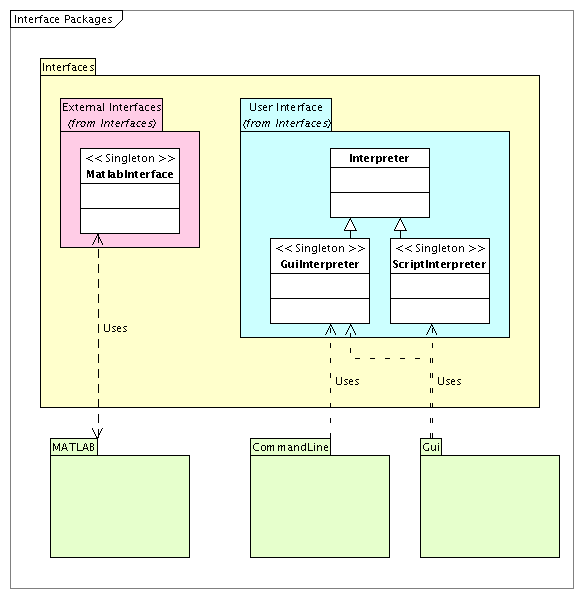
\includegraphics[420,430]{Images/InterfacePackages.png}
%\caption{\label{InterfacePackages}Interface Packages}
%\end{center}
%\end{figure}

\subsection{User Interfaces}

GMAT can be run from either a command line interface or a graphical user interface (GUI).  These
interfaces are connected to the core GMAT code through objects in the User Interface
portion of the Interface subsystem. The command line interface controls GMAT exclusively through
the singleton ScriptInterpreter  The GUI uses the ScriptInterpreter to read and write GMAT files
and to preview GMAT scripts, and the GuiInterpreter for other interactions with the internal GMAT
objects.

The command line interface provides minimal feedback during a run.  Users can use the command line
interface to execute GMAT scripts, either one at a time or in a batch mode.  The interface displays
status messages during the run, but provides no other feedback regarding the status of a script
run.  In batch mode, the interface runs multiple scripts sequentially based on the input from a
batch file.  Statistics regarding the success or failure of the individual scripts are collected
and displayed at the end of the run.

The graphical user interface is implemented using the wxWidgets GUI Library \cite{wxWidgets}.
It provides a rich development environment for the implementation of the user interface.  The GMAT
GUI is built on all three target platforms (Windows XP, MacIntosh OS X, and Linux) using the same
GUI code, with minimal customization for the different platforms.  The communications layer between
this library and core GMAT functionality is the GuiInterpreter.  Further information about the GUI
can be found in Chapter~\ref{chapter:TheGui}.

All scripting capabilities in GMAT are implemented using the ScriptInterpreter and its helper
classes.  This component is discussed in Chapter~\ref{chapter:ScriptRW}.  The GMAT scripting
language is documented in the \textbf{GMAT Mathematical Specifications and User's Guide}
\cite{mathSpec}, a companion volume to this document.

\subsection{External Interfaces}





%%\part{Subsystem Designs}

% % $Id: PropagatorOverview.tex,v 1.1 2008/10/09 16:16:11 dconway Exp $
\chapter{\label{chapter:Estimation}Estimation in GMAT}
\chapauthor{Darrel J. Conway}{Thinking Systems, Inc.}
\chapauthor{Matthew Wilkins}{Schafer Corporation}
\chapauthor{Steven P. Hughes}{Goddard Space Flight Center}

Here's where we'll put the top level OD descriptions.
\backmatter

%\printglossaries

\begin{thebibliography}{Math  Spec} % start the bibliography

\bibitem[ArchSpec]{archSpec} GMAT Development Team, ``GMAT Architectural Specification'', 2009.

\bibitem[Conway]{philosophy} Darrel J.Conway, ``The GMAT Design Philosophy'', Internal
Communications between Thinking Systems and Goddard, May 9, 2004.

\bibitem[Eckel]{thinkC}Bruce Eckel, ``Thinking in C++'', Prentice-Hall, New Jersey, 2000.

\bibitem[MathSpec]{mathSpec} Steven P. Hughes, ``General Mission Analysis Tool (GMAT) Mathematical
Specifications.''

\bibitem[NRecipes]{recipes} William H. Press, Saul A. Teukolsky, William T. Vetterling, and Brian
P. Flannery, \textbf{Numerical Recipes in C}, 2nd Edition, Cambridge University Press, 1992.

\bibitem[Vallado]{Vallado}D. Vallado, \textbf{Fundamentals of Astrodynamics and Applications},
2nd Ed., Microcosm Press, 2001.

\end{thebibliography}

\printindex

\end{document}
